%======================================================================
% University of Waterloo Thesis Template for LaTeX 
% Last Updated August 21, 2018 
% by Stephen Carr, IST Client Services, 
% University of Waterloo, 200 University Ave. W., Waterloo, Ontario, Canada
% FOR ASSISTANCE, please send mail to rt-IST-CSmathsci@rt.uwaterloo.ca

% DISCLAIMER
% To the best of our knowledge, this template satisfies the current uWaterloo thesis requirements.
% However, it is your responsibility to assure that you have met all 
% requirements of the University and your particular department.

% Many thanks for the feedback from many graduates who assisted the development of this template.
% Also note that there are explanatory comments and tips throughout this template.
%======================================================================
% Some important notes on using this template and making it your own...

% The University of Waterloo has required electronic thesis submission since October 2006. 
% See the uWaterloo thesis regulations at
% https://uwaterloo.ca/graduate-studies/thesis.
% This thesis template is geared towards generating a PDF 
% version optimized for viewing on an electronic display, including 
% hyperlinks within the PDF.

% DON'T FORGET TO ADD YOUR OWN NAME AND TITLE in the "hyperref" package
% configuration below. THIS INFORMATION GETS EMBEDDED IN THE PDF FINAL PDF DOCUMENT.
% You can view the information if you view properties of the PDF document.

% Many faculties/departments also require one or more printed
% copies. This template attempts to satisfy both types of output. See additional notes below.
% It is based on the standard "book" document class which provides all necessary 
% sectioning structures and allows multi-part theses.

% If you are using this template in Overleaf (cloud-based collaboration service), then it is 
% automatically processed and previewed for you as you edit.

% For people who prefer to install their own LaTeX distributions on their own computers, and process 
% the source files manually, the following notes provide the sequence of tasks:
 
% E.g. to process a thesis called "mythesis.tex" based on this template, run:

% pdflatex mythesis	-- first pass of the pdflatex processor
% bibtex mythesis	-- generates bibliography from .bib data file(s)
% makeindex         -- should be run only if an index is used 
% pdflatex mythesis	-- fixes numbering in cross-references, bibliographic references, glossaries, index, etc.
% pdflatex mythesis	-- it takes a couple of passes to completely process all cross-references

% If you use the recommended LaTeX editor, Texmaker, you would open the mythesis.tex
% file, then click the PDFLaTeX button. Then run BibTeX (under the Tools menu).
% Then click the PDFLaTeX button two more times. If you have an index as well,
% you'll need to run MakeIndex from the Tools menu as well, before running pdflatex
% the last two times.

% N.B. The "pdftex" program allows graphics in the following formats to be
% included with the "\includegraphics" command: PNG, PDF, JPEG, TIFF
% Tip 1: Generate your figures and photos in the size you want them to appear
% in your thesis, rather than scaling them with \includegraphics options.
% Tip 2: Any drawings you do should be in scalable vector graphic formats:
% SVG, PNG, WMF, EPS and then converted to PNG or PDF, so they are scalable in
% the final PDF as well.
% Tip 3: Photographs should be cropped and compressed so as not to be too large.

% To create a PDF output that is optimized for double-sided printing: 
%
% 1) comment-out the \documentclass statement in the preamble below, and
% un-comment the second \documentclass line.
%
% 2) change the value assigned below to the boolean variable
% "PrintVersion" from "false" to "true".

%======================================================================
%   D O C U M E N T   P R E A M B L E
% Specify the document class, default style attributes, and page dimensions, etc.
% For hyperlinked PDF, suitable for viewing on a computer, use this:
\documentclass[letterpaper,12pt,titlepage,oneside,final]{book}
 
% For PDF, suitable for double-sided printing, change the PrintVersion variable below
% to "true" and use this \documentclass line instead of the one above:
%\documentclass[letterpaper,12pt,titlepage,openright,twoside,final]{book}

% Some LaTeX commands I define for my own nomenclature.
% If you have to, it's easier to make changes to nomenclature once here than in a 
% million places throughout your thesis!
\newcommand{\package}[1]{\textbf{#1}} % package names in bold text
\newcommand{\cmmd}[1]{\textbackslash\texttt{#1}} % command name in tt font 
\newcommand{\href}[1]{#1} % does nothing, but defines the command so the
    % print-optimized version will ignore \href tags (redefined by hyperref pkg).
%\newcommand{\texorpdfstring}[2]{#1} % does nothing, but defines the command
% Anything defined here may be redefined by packages added below...

% This package allows if-then-else control structures.
\usepackage{ifthen}
\newboolean{PrintVersion}
\setboolean{PrintVersion}{false}
% CHANGE THIS VALUE TO "true" as necessary, to improve printed results for hard copies
% by overriding some options of the hyperref package, called below.

%\usepackage{nomencl} % For a nomenclature (optional; available from ctan.org)
\usepackage{amsmath,amssymb,amstext} % Lots of math symbols and environments
\usepackage[pdftex]{graphicx}
\usepackage{xcolor}
\usepackage[linesnumbered,plain,vlined,algo2e,figure]{algorithm2e}
\usepackage{graphicx} % DO NOT CHANGE THIS
\usepackage{subcaption}
% For including graphics N.B. pdftex graphics driver 

% Hyperlinks make it very easy to navigate an electronic document.
% In addition, this is where you should specify the thesis title
% and author as they appear in the properties of the PDF document.
% Use the "hyperref" package 
% N.B. HYPERREF MUST BE THE LAST PACKAGE LOADED; ADD ADDITIONAL PKGS ABOVE
\usepackage[pdftex,pagebackref=false]{hyperref} % with basic options
%\usepackage[pdftex,pagebackref=true]{hyperref}
		% N.B. pagebackref=true provides links back from the References to the body text. This can cause trouble for printing.
\hypersetup{
    plainpages=false,       % needed if Roman numbers in frontpages
    unicode=false,          % non-Latin characters in Acrobat’s bookmarks
    pdftoolbar=true,        % show Acrobat’s toolbar?
    pdfmenubar=true,        % show Acrobat’s menu?
    pdffitwindow=false,     % window fit to page when opened
    pdfstartview={FitH},    % fits the width of the page to the window
%    pdftitle={uWaterloo\ LaTeX\ Thesis\ Template},    % title: CHANGE THIS TEXT!
%    pdfauthor={Author},    % author: CHANGE THIS TEXT! and uncomment this line
%    pdfsubject={Subject},  % subject: CHANGE THIS TEXT! and uncomment this line
%    pdfkeywords={keyword1} {key2} {key3}, % list of keywords, and uncomment this line if desired
    pdfnewwindow=true,      % links in new window
    colorlinks=true,        % false: boxed links; true: colored links
    linkcolor=blue,         % color of internal links
    citecolor=green,        % color of links to bibliography
    filecolor=magenta,      % color of file links
    urlcolor=cyan           % color of external links
}
\ifthenelse{\boolean{PrintVersion}}{   % for improved print quality, change some hyperref options
\hypersetup{	% override some previously defined hyperref options
%    colorlinks,%
    citecolor=black,%
    filecolor=black,%
    linkcolor=black,%
    urlcolor=black}
}{} % end of ifthenelse (no else)
\usepackage{xspace}
\usepackage{booktabs}
\usepackage[capitalise]{cleveref}
\usepackage{listings}
\usepackage{adjustbox}
\lstset{basicstyle=\footnotesize\ttfamily,breaklines=true,
        keywordstyle=\color{blue}\ttfamily,
        stringstyle=\color{red}\ttfamily,
        commentstyle=\color{brown}\ttfamily,
        morecomment=[l][\color{magenta}],
        numbers=left,
        showstringspaces=false}
\usepackage[automake,toc,abbreviations]{glossaries-extra} % Exception to the rule of hyperref being the last add-on package


% If glossaries-extra is not in your LaTeX distribution, get it from CTAN (http://ctan.org/pkg/glossaries-extra), 
% although it's supposed to be in both the TeX Live and MikTeX distributions. There are also documentation and 
% installation instructions there.

% Setting up the page margins...
% uWaterloo thesis requirements specify a minimum of 1 inch (72pt) margin at the
% top, bottom, and outside page edges and a 1.125 in. (81pt) gutter
% margin (on binding side). While this is not an issue for electronic
% viewing, a PDF may be printed, and so we have the same page layout for
% both printed and electronic versions, we leave the gutter margin in.
% Set margins to minimum permitted by uWaterloo thesis regulations:
\setlength{\marginparwidth}{0pt} % width of margin notes
% N.B. If margin notes are used, you must adjust \textwidth, \marginparwidth
% and \marginparsep so that the space left between the margin notes and page
% edge is less than 15 mm (0.6 in.)
\setlength{\marginparsep}{0pt} % width of space between body text and margin notes
\setlength{\evensidemargin}{0.125in} % Adds 1/8 in. to binding side of all 
% even-numbered pages when the "twoside" printing option is selected
\setlength{\oddsidemargin}{0.125in} % Adds 1/8 in. to the left of all pages
% when "oneside" printing is selected, and to the left of all odd-numbered
% pages when "twoside" printing is selected
\setlength{\textwidth}{6.375in} % assuming US letter paper (8.5 in. x 11 in.) and 
% side margins as above
\raggedbottom

% The following statement specifies the amount of space between
% paragraphs. Other reasonable specifications are \bigskipamount and \smallskipamount.
\setlength{\parskip}{\medskipamount}

% The following statement controls the line spacing.  The default
% spacing corresponds to good typographic conventions and only slight
% changes (e.g., perhaps "1.2"), if any, should be made.
\renewcommand{\baselinestretch}{1} % this is the default line space setting

% By default, each chapter will start on a recto (right-hand side)
% page.  We also force each section of the front pages to start on 
% a recto page by inserting \cleardoublepage commands.
% In many cases, this will require that the verso (left-hand) page be
% blank, and while it should be counted, a page number should not be
% printed.  The following statements ensure a page number is not
% printed on an otherwise blank verso page.
\let\origdoublepage\cleardoublepage
\newcommand{\clearemptydoublepage}{%
  \clearpage{\pagestyle{empty}\origdoublepage}}
\let\cleardoublepage\clearemptydoublepage

% Define Glossary terms (This is properly done here, in the preamble and could also be \input{} from a separate file...)
% Main glossary entries -- definitions of relevant terminology
\newglossaryentry{computer}
{
name=computer,
description={A programmable machine that receives input data,
               stores and manipulates the data, and provides
               formatted output}
}

% Nomenclature glossary entries -- New definitions, or unusual terminology
\newglossary*{nomenclature}{Nomenclature}
\newglossaryentry{dingledorf}
{
type=nomenclature,
name=dingledorf,
description={A person of supposed average intelligence who makes incredibly brainless misjudgments}
}

% List of Abbreviations (abbreviations type is built in to the glossaries-extra package)
\newabbreviation{aaaaz}{AAAAZ}{American Association of Amateur Astronomers and Zoologists}

% List of Symbols
\newglossary*{symbols}{List of Symbols}
\newglossaryentry{rvec}
{
name={$\mathbf{v}$},
sort={label},
type=symbols,
description={Random vector: a location in n-dimensional Cartesian space, where each dimensional component is determined by a random process}
}
 
\makeglossaries

%======================================================================
%   L O G I C A L    D O C U M E N T
% The logical document contains the main content of your thesis.
% Being a large document, it is a good idea to divide your thesis
% into several files, each one containing one chapter or other significant 
% chunk of content, so you can easily shuffle things around later if desired.
%======================================================================
\newcommand{\vect}[1]{\boldsymbol{#1}}
\newcommand{\ag}[1]{{\color{blue} [\textbf{AG}: #1]}}
\newcommand{\NL}[1]{{\color{orange} [\textbf{NL}: #1]}}
\newcommand{\xs}[1]{{\color{purple} [\textbf{XS}: #1]}}
\newcommand{\term}[1]{\langle \text{#1} \rangle}

% Uncomment to hide comments
% \renewcommand{\ag}[1]{}
% \renewcommand{\NL}[1]{}
% \renewcommand{\xs}[1]{}

\newcommand{\indgen}{\mathit{indgen}}

\newcommand{\chccomp}{\textsc{CHC-COMP 2018}\xspace}
\newcommand{\Ppos}{P^+}
\newcommand{\Pneg}{P^-}
\newcommand{\Mpos}{M^+}
\newcommand{\Mneg}{M^-}
%spacer macros
\newcommand{\trs}{\langle \Init, \Tr, \Bad \rangle\xspace}
\newcommand{\trinit}{\langle \Init, \Tr\rangle\xspace}
\newcommand{\ig}{inductive generalization\xspace}
\newcommand{\indf}{\textit{inductive}\xspace}
\newcommand{\spc}{\textsc{Spacer}\xspace}
\newcommand{\dpy}{\textsc{Dopey}\xspace}
\newcommand{\GSpacer}{\textsc{GSpacer}\xspace}
\newcommand{\csm}{\textsc{GSpacer}\xspace}
\newcommand{\ddchc}{\textsc{LArb}\xspace}
\newcommand{\concr}{\textsc{Concretize}}
\newcommand{\concrlit}{\textsc{Concretize\_lit}}
\newcommand{\concrcube}{\textsc{Concretize\_cube}}
\newcommand{\fVar}[1]{\textsc{Vars}(#1)}
\newcommand{\lind}[1]{#1^{L_{\downarrow}}}
\newcommand{\const}[1]{\textsc{Consts}(#1)}
\newcommand{\coeff}[2]{\textsc{coeff}(#1, #2)}
\newcommand{\pobclstr}[2]{\cC_{\textit{pob}}(\langle #1, #2\rangle)}
\newcommand{\lclstr}[1]{\cC_{\textit{lemma}}(#1)}
\newcommand{\conjpre}[3]{\textsc{ShouldConjecture}(#1, #2, #3)}
\newcommand{\conjProc}[3]{\textsc{Conjecture}(#1, #2, #3)}
\newcommand{\isSat}{\textsc{isSat}}
\newcommand{\nonLin}{\textsc{nonLin}}
\newcommand{\mbp}{\textsc{MBP}}
\newcommand{\getS}{\textsc{GetS}}
\newcommand{\getP}{\textsc{GetP}}
\newcommand{\itp}{\textsc{ITP}}
\newcommand{\gen}{\textsc{GEN}}
\newcommand{\seqItp}{\textsc{seqItp}}
\newcommand{\resolve}{\bowtie}
\newcommand{\Var}{\textsf{Var}}
\newcommand{\pob}{\textsc{pob}\xspace}
\newcommand{\pobs}{\textsc{pob}s\xspace}

\newcommand{\true}{\mathit{true}}
\newcommand{\false}{\mathit{false}}
\newcommand{\Tr}{\mathit{Tr}}
\newcommand{\Bad}{\mathit{Bad}}
\newcommand{\Init}{\mathit{Init}}
\newcommand{\Inv}{\mathit{Inv}}
\newcommand{\Rinv}{\mathit{RelInv}}
\newcommand{\iframe}{\operatorname{frm}}

\newcommand{\unsafe}{\textsc{unsafe}\xspace}
\newcommand{\safe}{\textsc{safe}\xspace}
\newcommand{\limp}{\Rightarrow}

\newcommand{\Sig}{\Sigma}
\newcommand{\SigU}{X}
\newcommand{\SigI}{S}
\newcommand{\lit}{\textit{lit}}
\newcommand{\Lem}{\mathit{Lem}}
\newcommand{\GLem}{\mathit{GLem}}
\newcommand{\Lit}{\mathit{Lit}}
\newcommand{\GLit}{\mathit{GLit}}



\newcommand{\Consts}{\vect{x}}
\newcommand{\tool}{\textsc{QuickDrop}\xspace}
\newcommand{\cC}{\mathcal{C}}
\newcommand{\cO}{\mathcal{O}}
\newcommand{\cI}{\mathcal{I}}
\newcommand{\cA}{\mathcal{A}}
\newcommand{\cD}{\mathcal{D}}
\newcommand{\cL}{\mathcal{L}}
\newcommand{\cT}{\mathcal{T}}
\newcommand{\cQ}{\mathcal{Q}}
\newcommand{\cS}{\mathcal{S}}
\newcommand{\cN}{\mathcal{N}}
\newcommand{\cU}{\mathcal{U}}
\newcommand{\cF}{\mathcal{F}}
\newcommand{\cP}{\mathcal{P}}
\newcommand{\RNUM}{\texttt{<RNUM> }}
\newcommand{\INUM}{\texttt{<INUM> }}
\newcommand{\SIGN}{\texttt{<SIGN> }}
\newcommand{\cl}{\ell}
\newcommand{\vx}{\vec{x}}
\newtheorem{theorem}{Theorem}
\newtheorem{problem}{Problem}

\newcommand{\Spacer}{\textsc{Spacer}\xspace}
\newcommand{\Lcal}{\mathcal{L}}

\newcommand{\twopartdef}[4]
{
	\left\{
		\begin{array}{ll}
			#1 & \mbox{if } #2 \\
			#3 & \mbox{if } #4
		\end{array}
	\right.
}

\newcommand{\ltrue}{\textsf{true}}
\newcommand{\lfalse}{\textsf{false}}

\newcommand{\gnutree}{\textsc{GNU Tree}\xspace}
\newcommand{\insttovec}{\textsc{inst2vec}\xspace}
\newcommand{\reinforce}{\textsc{reinforce}\xspace}
\newcommand{\cmix}{\textsc{C-Mix}\xspace}
\newcommand{\tempo}{\textsc{Tempo}\xspace}
\newcommand{\llvm}{\textsc{LLVM}\xspace}

\newcommand{\llpe}{\textsc{LLPE}\xspace}
\newcommand{\occam}{\textsc{Occam}\xspace}
\newcommand{\trimmer}{\textsc{Trimmer}\xspace}
\newcommand{\occamo}{\textsc{occamNone}\xspace}
\newcommand{\occama}{\textsc{occamAgg}\xspace}
\newcommand{\chisel}{\textsc{Chisel}\xspace}
\newcommand{\doccam}{\textsc{DeepOccam}\xspace}
\newcommand{\codetovec}{\textsc{Code2Vec}\xspace}
\newcommand{\pytorch}{\textsc{PyTorch}\xspace}
\newcommand{\gsa}{\textsc{gsa}\xspace}

\newcommand{\cpp}{C\texttt{++}\xspace}

\begin{document}

%----------------------------------------------------------------------
% FRONT MATERIAL
% title page,declaration, borrowers' page, abstract, acknowledgements,
% dedication, table of contents, list of tables, list of figures, nomenclature, etc.
%----------------------------------------------------------------------
% T I T L E   P A G E
% -------------------
% Last updated June 14, 2017, by Stephen Carr, IST-Client Services
% The title page is counted as page `i' but we need to suppress the
% page number. Also, we don't want any headers or footers.
\pagestyle{empty}
\pagenumbering{roman}

% The contents of the title page are specified in the "titlepage"
% environment.
\begin{titlepage}
        \begin{center}
        \vspace*{1.0cm}

        \Huge
        {\bf Neural-guidance for symbolic reasoning}

        \vspace*{1.0cm}

        \normalsize
        by \\

        \vspace*{1.0cm}

        \Large
        Nham Le \\

        \vspace*{3.0cm}

        \normalsize
        A thesis \\
        presented to the University of Waterloo \\ 
        in fulfillment of the \\
        thesis requirement for the degree of \\
        Master of Applied Science \\
        in \\
        Electrical and Computer Engineering \\

        \vspace*{2.0cm}

        Waterloo, Ontario, Canada, 2020 \\

        \vspace*{1.0cm}

        \copyright\ Nham Le 2020 \\
        \end{center}
\end{titlepage}

% The rest of the front pages should contain no headers and be numbered using Roman numerals starting with `ii'
\pagestyle{plain}
\setcounter{page}{2}

\cleardoublepage % Ends the current page and causes all figures and tables that have so far appeared in the input to be printed.
% In a two-sided printing style, it also makes the next page a right-hand (odd-numbered) page, producing a blank page if necessary.

 
% E X A M I N I N G   C O M M I T T E E (Required for Ph.D. theses only)
% Remove or comment out the lines below to remove this page
% \begin{center}\textbf{Examining Committee Membership}\end{center}
%   \noindent
% The following served on the Examining Committee for this thesis. The decision of the Examining Committee is by majority vote.
%   \bigskip
  
%   \noindent
% \begin{tabbing}
% Internal-External Member: \=  \kill % using longest text to define tab length
% External Examiner: \>  Bruce Bruce \\ 
% \> Professor, Dept. of Philosophy of Zoology, University of Wallamaloo \\
% \end{tabbing} 
%   \bigskip
  
%   \noindent
% \begin{tabbing}
% Internal-External Member: \=  \kill % using longest text to define tab length
% Supervisor(s): \> Doris Johnson \\
% \> Professor, Dept. of Zoology, University of Waterloo \\
% \> Andrea Anaconda \\
% \> Professor Emeritus, Dept. of Zoology, University of Waterloo \\
% \end{tabbing}
%   \bigskip
  
%   \noindent
%   \begin{tabbing}
% Internal-External Member: \=  \kill % using longest text to define tab length
% Internal Member: \> Pamela Python \\
% \> Professor, Dept. of Zoology, University of Waterloo \\
% \end{tabbing}
%   \bigskip
  
%   \noindent
% \begin{tabbing}
% Internal-External Member: \=  \kill % using longest text to define tab length
% Internal-External Member: \> Deepa Thotta \\
% \> Professor, Dept. of Philosophy, University of Waterloo \\
% \end{tabbing}
%   \bigskip
  
%   \noindent
% \begin{tabbing}
% Internal-External Member: \=  \kill % using longest text to define tab length
% Other Member(s): \> Leeping Fang \\
% \> Professor, Dept. of Fine Art, University of Waterloo \\
% \end{tabbing}

% \cleardoublepage

% D E C L A R A T I O N   P A G E
% -------------------------------
  % The following is a sample Delaration Page as provided by the GSO
  % December 13th, 2006.  It is designed for an electronic thesis.
  \noindent
This  thesis  consists  of  material  all  of  which  I  authored  or  co-authored: see  Statement of Contributions included in the thesis.  This is a true copy of the thesis,  including any required final revisions, as accepted by my examiners. 



  \bigskip
  
  \noindent
I understand that my thesis may be made electronically available to the public.

\cleardoublepage
\begin{center}
\textbf{Statement of Contributions}
\end{center}
Some of the text, figures and tables in this thesis are restated from our NeurIPS workshop paper \cite{Nham:nips19} and our current submission.

\textsc{Occam} was written by the researchers at The Computer Science Laboratory at SRI International.

Some of the source code for \textsc{Spacer} was written by Arie Gurfinkel.
\cleardoublepage
% A B S T R A C T
% ---------------

\begin{center}\textbf{Abstract}\end{center}
Symbolic reasoning was the founding father of Artificial Intelligence (AI). With the recent advances in Deep Learning, many traditional AI areas such as Computer Vision and Natural Language Processing have moved to probabilistic-based approaches. However, in applications where there is little to no room for uncertainty, such as Compiler or Software verification, symbolic reasoning is still the go-to option. In this thesis, we bring the advantage of data-driven learnable models into the precise world of symbolic reasoning. In particular, we choose to tackle two specific problems: Model Checking, in the context of Inductive Generalization, and Compiler Optimization, in the context of Software Debloating. We implemented our approach in two tools, named \textsc{Dopey} and \textsc{DeepOccam}, respectively. They both use traces generated from running a task to learn a better heuristic, and use said heuristic to improve subsequent runs of the same or similar tasks. Our results show that both neural-based heuristics outperform handcrafted heuristics.

\cleardoublepage

% A C K N O W L E D G E M E N T S
% -------------------------------

\begin{center}\textbf{Acknowledgements}\end{center}
I would like to thank Professor Arie Gurfinkel sharing their  expertise  in  the  subject,  availability  and  giving  valuable  advices  for  this  research. It goes without saying that this document would not be possible without him. 

I would like to thank Professor Werner Dietl and Professor Vijay Ganesh for attending the seminar, reviewing the thesis and providing valuable feedback on both occasions. 

I would like to thank the people at SRI International, especially Dr. Ashish Gehani and Dr. Jorge Navas, for the wonderful time I had there.

Finally, I would like to thank Dr. Xujie Sie for his deep insight into the world of neural-symbolic. This thesis would be nowhere near its current form without him.
% I would like to thank all the little people who made this thesis possible.
\cleardoublepage

% D E D I C A T I O N
% -------------------

\begin{center}\textbf{Dedication}\end{center}

This is dedicated to the one I love.
\cleardoublepage

% T A B L E   O F   C O N T E N T S
% ---------------------------------
\renewcommand\contentsname{Table of Contents}
\tableofcontents
\cleardoublepage
\phantomsection    % allows hyperref to link to the correct page

% L I S T   O F   T A B L E S
% ---------------------------
\addcontentsline{toc}{chapter}{List of Tables}
\listoftables
\cleardoublepage
\phantomsection		% allows hyperref to link to the correct page

% L I S T   O F   F I G U R E S
% -----------------------------
\addcontentsline{toc}{chapter}{List of Figures}
\listoffigures
\cleardoublepage
\phantomsection		% allows hyperref to link to the correct page

% GLOSSARIES (Lists of definitions, abbreviations, symbols, etc. provided by the glossaries-extra package)
% -----------------------------
\printglossaries
\cleardoublepage
\phantomsection		% allows hyperref to link to the correct page

% Change page numbering back to Arabic numerals
\pagenumbering{arabic}

 

%----------------------------------------------------------------------
% MAIN BODY
% We suggest using a separate file for each chapter of your thesis.
% Start each chapter file with the \chapter command.
% Only use \documentclass or \begin{document} and \end{document} commands 
% in this master document.
% Tip 4: Putting each sentence on a new line is a way to simplify later editing.
%----------------------------------------------------------------------
\chapter{Introduction}
% \section{Neural networks are the new symbolic heuristics}
Symbolic reasoning predates Computer Science. The word \emph{algorithm} itself came from the 9th-century mathematician Muhammad ibn Musa al-Khwarizmi, Latinized Algoritmi. Logics itself could be traced back to Aristotle in the 300s BC. It is fair to say that the whole field of Computer Science was born out of symbolic reasoning, with pioneering work such as Hilbert's \emph{Entscheidungsproblem}, Alonzo Church's \emph{Lambda Calculus}, and Alan Turing's \emph{Turing machine}.
A century has passed since the birth of modern Computer Science, and the field is now so diverse in the use of mathematics: Topology and Geometry in Computer Graphics, Probability and Linear Algebra in Deep learning, among others.
Nowadays, symbolic reasoning could still be found in Computer Science in its pure form under the research of Programming Languages, Compilers, Formal Methods, and Automated Reasoning. 

Throughout its history, at the heart of all the symbolic reasoning applications are carefully handcrafted heuristics, tried-and-true by years of human experts' research. While those heuristics work wonderfully, they come with the cost of being too specific to the problem at hand. For example, there is no easy way to transfer all the wisdom learned in crafting a SAT-solver heuristic or the heuristic itself to create a better heuristic for a CHC-solver. This raises a natural, practical, and to a certain extend, a philosophical question: can a heuristic for a symbolic reasoning system be learned automatically?

Just ten years ago, only the most ambitious researchers would answer ``yes'' for the above question. While glimpse of learnable heuristics could already be found in groundbreaking work such as TD-Gammon \cite{td-gammon}, the whole research direction was practically halted due to hardware limitation. Then, at the turn of the 2010s, researchers realized that the heaviest workload in Deep learning --- matrix multiplication --- could be done very efficiently using GPU --- an easy to find and cheap hardware component. AlexNet \cite{Krizhevsky:nips12} - one of the first works that demonstrated the scalability of Deep Neural Networks using GPUs - blew every other image recognition methods at the time out of the water, and overnight, old ideas were new again: Convolution Neural Network, Long-Short Term Memory (LSTM) Network, Deep Reinforcement Learning, etc. are all in the realm of possibility. Nowadays, it is hard to find a field that is not yet ``transformed'' or ``revolutionized'' by Deep learning.

Yet, symbolic reasoning is still one of the less successful applications of Deep learning: while Deep learning has been able to achieve human-level, or even superhuman-level on many tasks, such as Image Recognition, Automated Speech Recognition, Game Playing (Go, Atari), it still fails short of the state-of-the-art heuristics at many symbolic reasoning tasks, such as solving mathematical equations \cite{lample2019deep} or solving SAT problems \cite{neuralsat}. Ironically, symbolic reasoning was also the reason for the first \textbf{AI Winter}: Marvin Minsky, founder of the MIT AI Lab, and Seymour Papert, director of the lab at the time, in 1969 published the seminal book Perceptrons \cite{perceptrons}, that discussed perceptron's inability to learn the simple boolean function XOR because it is not linearly separable, turning research away from the perceptron. The history of symbolic reasoning and Deep learning, as often said, comes full circle.

We hypothesize that it is possible to learn Deep learning-based heuristics those are better than handcrafed one. This thesis offers a glimpse into this possibility, by presenting two concrete positive results where effective heuristics are indeed learnable from data, in two particular domains: compiler optimization, and automated reasoning. We choose to tackle those two domains because we believe the handcrafted heuristics there are not optimal and there are still a lot of room for improvement, and as shown in the following chapters, we indeed improved them by a large margin.

\section{Symbolic Model Checking using co-occurrence probabilities}
In the automated reasoning domain, we introduce \dpy, a neural-based Symbolic Model Checker (SMC) / Constraint Horn Clauses (CHC) Solver.

Model checking has been widely used in various important areas such as robustness analysis of deep neural networks~\cite{Katz:cav19}, verification of hardware designs~\cite{SMC96}, software verification~\cite{Ball02}, analysis~\cite{ESC-java-02} and testing~\cite{Sheyner:SP02}, parameter synthesis in biology~\cite{Barnat:biology12}, and many others. 
The central challenge of model checking is to find a concise and sound approximation of all possible states a given system may reach, which does not cover any undesired states (i.e. violating given specifications). 
Tremendous processes have been made by innovations in efficient data representations~\cite{BDD}, scalable SAT solvers~\cite{CDCL,chaff,minisat}, and effective heuristics~\cite{CEGAR,BMC,McMillan:cav06}.  
Modern model checkers share a common basis, namely, IC3~\cite{IC3}, of which the key insight is \textit{inductive generalization (inductive generalization)}.
This idea has been generalized to support rich theories~\cite{GPDR} that are crucial for many verification tasks~\cite{Komuravelli:cav13,SeaHorn} beyond hardware verification. 
The generalized IC3 with rich theories, also known as satisfiability checking for Constrained Horn Clauses modulo Theory
(CHC)~\cite{DBLP:conf/birthday/BjornerGMR15}, becomes the core part of a broad range of verification tasks.


% \NL{essentially it is a search problem, and traditionally handcrafted heuristics are used. ML can give better heuristic blabh blah}
% With deep learning models being applied in many real life application, verifying them is very important, and push traditional model checking methods to its boundary.

Existing inductive generalization techniques follow either an enumerative search process \cite{IC3,Bradley:fmcad11} or ad-hoc heuristics \cite{Griggio:CAD16,GSpacer}. 
Heuristics are effective but may demand non-trivial domain-specific (or even problem-specific) expertise. 
In this work, we aim to automatically learn such heuristics from the past successful inductive generalizations. 
We observe that verification problems as well as associated inductive generalizations are not isolated from each other. 
Taking software verification as an example, verifying different properties of the same program involves similar or same inductive generalizations; different versions of programs have similar code base; and
different software may use same coding convention, idioms, library or framework, resulting in similar structures.


% Can inductive generalization heuristics be automatically learned?
% Our approach is inspired by the recent advances in deep learning, which automatically learn non-trivial patterns from raw pixels~\cite{Krizhevsky:nips12} as well as semantic correlations between natural language texts~\cite{Mikolov:nips13}.
A natural solution is to train a deep learning model to directly perform inductive generalization, but this approach also raises many new challenges for deep learning. 
% symbols, 
% structured data,
% semantic reasoning (semantic valid/correct), 
% soundness,
% training data.
First of all, the input and the output of inductive generalization are symbolic expressions, which are \textit{highly structured} with \textit{rich semantics}. 
Slight syntactic variations can lead to dramatic changes in semantics.
Second, more importantly, inductive generalization has to satisfy complicated \textit{semantic constraints}. 
Third, given deep learning models hardly provide any reliable guarantees, how to design a neuro-symbolic system that exhibits \textit{learnability} from past experiences but still preserves \textit{soundness}?
% Fourth, how to learn a neural model through a sequence of complicated logical reasoning which are clearly \textit{not differentiable}?
All these challenges have to be properly addressed in building a neuro-symbolic reasoning framework. 
% In this work, we share our design choices and empirical findings in building 

In \cref{chap:dopey}, we present a neuro-symbolic engine \dpy, which introduces a neural component into symbolic model checking. Specifically, we make the following contributions: 
\begin{itemize}
    % \item we study the performance bottleneck of symbolic model checking and
    % factor out a component that are suitable for learning from the past runs;
    \item we adapt standard deep learning models to effectively represent symbolic expressions by incorporating both syntactic and semantic information;
    \item we design a simple but effective learning objective so that training data can be collected with nearly no changes of existing model checkers; 
    \item our integration algorithm achieves the soundness by design, and in the worst case, the learning component may only hurt the running time performance; 
    \item we implement \dpy on top of \spc, a state-of-the-art CHC-solver, using an efficient client-server architecture;
    \item our empirical evaluations indicate \dpy significantly improves \spc on 
    challenging benchmarks from \chccomp.
\end{itemize}


\section{Compiler Optimization using Reinforcement Learning}
In the compiler optimization domain, we introduce \doccam, a reinforcement-learning--based software debloating tool. 
% The rapid increase of software productivity in the last decades was fueled by the
% extensive use of abstraction and reuse of software components. While this
% enabled building larger and more complex software systems, these gains came at
% the expense of less efficient and less secure software systems, and contribute
% to a troublesome trade-off between productivity and performance/security. When
% an application built using general-purpose components is deployed, the majority
% of the general-purpose functionality is never used. This creates two problems:
% first, as the use of abstraction layers makes it more difficult to optimize the
% software, this has a detrimental impact on performance; second, it increases the
% attack surface for security vulnerabilities.

A \emph{Software Debloater} solves a specific problem: given the known running environment, can we remove as much unused code (\emph{debloat}) in the compiled executables and binaries as possible? A motivating example is the frequently used tool \texttt{ls}. \texttt{ls} has more than 40 arguments, yet for many people, \texttt{ls -lath} covers most of the use-cases. By removing code of the rest of \texttt{ls}'s arguments, a software debloater hopes to create a smaller, and safer \texttt{ls}.

% Ashish: While OCCAM, Trimmer, (and Chisel, via tests that the delta-debugged version must pass) specialize the application to its deployment context, other debloaters, such as Piece-wise, do not.
% An emerging solution to this problem is a set of tools, called \emph{Software
%   Debloaters}, that automatically customize a program to a user-specified
% environment. 

One successful approach for software debloating is based on partial
evaluation (PE)~\cite{pe-book} in which a \emph{partial evaluator} takes a
program and its known input values and produces a \emph{residual}
(or \emph{specialized}) program in which those inputs are replaced with constants.
%
% AG: not sure why soundness is important at this point of intro
% A sound partial evaluator must ensure that running the residual program on the
% remaining inputs always produces the same result as running the original
% program on all of its inputs.
%
While PE has been extensively applied to functional and logic programs, it was
less successful on imperative C/\cpp programs (with a noteable exception of
\cmix~\cite{Andersen94} and \tempo~\cite{Consel98}). With the advent of
\llvm~\cite{llvm}, several new partial evaluators of LLVM bitcode have arisen
during the last few years (e.g., \llpe~\cite{llpe}, \occam~\cite{occam}, and
\trimmer~\cite{trimmer}). These tools leverage \llvm optimizations such as
constant propagation, function inlining, and others to either reduce the size of
the residual program (e.g., \occam and \trimmer) or improve performance (e.g.,
\llpe).

The key step of a PE-based debloater is to estimate whether specializing (or
inlining) a function will result in a smaller (or more secure) residual program.
%Unfortunately, as with most problems in program analysis, this is very difficult.
Specialization naturally increases the size of the code since it adds extra
functions. However, since some inputs in the new functions have been replaced by
constant values, optimizations such as constant propagation, might become
enabled and result in new optimization opportunities that reduce the code size.
Therefore, the decision whether or not a function should be specialized for a
particular call-site is non-trivial. % where the solution must be found
% in a large search space that represents the effects of other specialized call
% sites and all LLVM optimizations applied after those specializations.
% Current PE-based software debloaters use naive heuristics. For example, \occam
% implements two heuristics of ``never specialize'' or ``always specialize'',
% respectively; \trimmer specializes a function only if it is called once in the
% whole program. 

% In this thesis, we present a new approach based on reinforcement
% learning (RL) to automatically infer effective heuristics for
% specializing functions for PE-based software debloating. RL is a natural direction since 

Interestingly, this decision of whether a call-site should be specialized or not resembles a long-horizon Markov Decision Process, which fits nicely into the Reinforcement Learning framework: each decision moves the code (state) from one to another, the decision should depend only on the current state instead of the whole history of transformation, and the quality of the whole process (reward) is only known at the end. 



% However, representing code as RL state is a 

% RL is a good fit for the problem for two reasons. First, code specialization
% resembles a Markov Decision Process: each decision moves the code from
% one state to another, and specialization depends only on the current
% state rather than the history of the transformations.  Second, the
% quality of debloating can only be measured after all specialization
% actions and corresponding compiler optimizations have been
% performed. % Rendering approaches like
% supervised-learning inapplicable.

To realize this insight, we need to solve the challenge of deciding on a good state representation.  While it is tempting to use the source code (or LLVM
intermediate representation (IR)) as a state, this is not
computationally tractable. The IR is typically hundreds of MBs in
size. Instead, an adequate set of features that captures meaningful
information about the code while avoiding state aliasing is
required. In particular, these features must capture the \emph{calling context}
in order to distinguish between call-sites. 

% Our finding is presented in \cref{chap:doccam}, in which we makes the following contributions:

In \cref{chap:doccam}, we present a software debloated \doccam, which learns a heuristic for specialization using Reinforcement Learning. Specifically, we make the following contributions: 
\begin{itemize}
    \item we propose a set of Calling context features that enable RL to find a useful heuristic for PE-based debloating software;
    \item we implementation of our method in a software debloater called \doccam;
    \item we evaluate on the reduction of the
program size and number of possible code-reuse attacks, by comparing
our handcrafted features with features learnt automatically via
embedding LLVM IR into a vector space using \insttovec~\cite{inst2vec}.
\end{itemize}
% The main contributions of this paper are threefold: (1) (2) ; and (3) 
% %
% Our initial evaluation suggests that RL is a viable method for
% developing an effective specialization policy for debloating, and learning with
% handcrafted features is easier than with \insttovec.

\section{Organizations of the thesis}
This thesis proposes two neural-guided heuristics for  software debloating - a compiler optimization task, and inductive generalization - a model checking algorithm's components. The key novelty is in automatically learning useful signals from a discrete logic world using a differientable framework. The rest of the thesis is structured as follows:

In \cref{chap:background}, we introduce needed background on our domains, which are Symbolic Model Checking and Software Debloating, our learning paradigms, which are Deep learning and Reinforcement learning, and finally our engineering glue that binds the realm of existing compilers and model checkers with a neural-guided heuristic: gRPC.

In \cref{chap:dopey}, we present a novel neural-symbolic SMC, called \dpy --- inspired by the
learning of co-occurrence probabilities in NLP. \dpy
learns offline dependence between atoms that do (or do not) appear together in
facts (called \emph{lemmas}) that are learned by the SMC. The neural net
is then used in successive runs of the SMC on different properties of the same system to guide 
the inductive generalization heuristic. Thus, in a
multi-property setting, learning from one verification task generalizes to
others.

In \cref{chap:doccam}, we present a neural-guided software debloating tool, called \doccam. \doccam uses Reinforcement learning to learn a heuristic for when to or not to apply \emph{specialization} -- a particular compiler optimization in which inputs those are known to be fixed (e.g a web server that is known to always run using HTTP 2.0) are replaced with their values. The metrics that \doccam tries to optimize is the number of ROP gadgets in the compiled binaries.

Finally, we outline a number of future research direction in \cref{chap:future}, and conclude in \cref{chap:conclusion}.
\chapter{Background}
In this chapter, we present preliminaries needed for the rest of the thesis.
\label{chap:background}
\section{Symbolic model checking}
\newcommand{\safety}{\textsc{Safety}\xspace}
In this section, we present the \safety problem, SAT-based model checking, and the IC3/PDR algorithm. They are needed for understanding \cref{chap:dopey}.
\paragraph{The \safety problem.}
% \nl{currently borrowed from gspacer}

% \textbf{Safety problem of transition system}
We consider first order logic modulo theories, using the standard notation and terminology. A first-order language modulo theory $\cT$ is defined over a signature $\Sig$ containing constant, function, and predicate symbols. 

A \emph{transition system} is a tuple $\langle \Sig, \Init,
\Tr \rangle$.
$\Sig$, $\Sig'$, and $\Sig^i$ are used to present the pre-state, the post-state, and the state of the system after executing $i$ steps, respectively ($\Sig' = \{v' \mid v \in \Sig\}$, $\Sig^i = \{v^i \mid v \in \Sig\}$). 
$\Init$ is a formula over $\Sig$ and $\Tr$ is a formula over $\Sig \cup \Sig'$. For a formula $\varphi$ over variables in $\Sig$, we denote by $\varphi'$ the formula obtained by substituting each $v \in \varphi$ by $v' \in \Sig'$, and $\varphi^i$ the formula obtained by substituting each $v \in \varphi$ by $v^i \in \Sig^i$. We also denote $\Tr^i$ a formula obtained by substituting each $v \in \Tr$ by $v^i \in \Sig^i$ and each $v' \in \Tr'$ by $v^{i+1} \in \Sig^{i+1}$.


For simplicity, we use the shorthand $\trinit$ to represent the transition system.
% \footnote{In fact, a
%   primed copy is introduced in $\Sig'$ only for the uninterpreted symbols in
%   $\Sig$. Interpreted symbols remain the same in $\Sig'$.} 
% The states of the system correspond
% to structures over $\Sig$, 
% $\Init$ represents the initial state and $\Tr$
% represents the transition relation, where $\Sig$ is used to represent the pre-state of a transition, and $\Sig'$ is used to represent the post-state. 

A \emph{\safety problem} is a triple 
$P = \langle \Init, \Tr, \Bad \rangle$, where
$\langle \Init, \Tr \rangle$ is a transition system and $\Bad$ is a
formula over $\Sig$ representing a set of bad states. $P$ is \emph{UNSAFE} if and only if there exists a number $N$ such that
\begin{align}
\label{form:safety}
    \Init^0\land (\bigwedge^{N-1}_{i=0}Tr^i)\land \Bad^N
\end{align}.
In this case, we also say that $P$ has a \emph{counterexample (CEX)} of length $N$. Vice versa, $P$ is \emph{SAFE} if and only if \cref{form:safety} is unsatisfiable.



The safety problem defined above is an instance of a more general problem,
CHC-SAT, of satisfiability of Constrained Horn Clauses (CHC). With abuse of notation, in this thesis we use \textit{solving CHC} and \textit{verify safety} interchangably.

% \textit{Linear Real Arithmetics}
% We provide the necessary background on the Safety problem of transition system (CHC solving), how IC3/Spacer works and where does Inductive generalization fit it, and the TreeLSTM neural network model.
% \textbf{sketch:}
% \begin{itemize}
%     \item Safety problem of transistion system (CHC solving)
%     \item Spacer/IC3, Indgen
%     \item Representation learning of symbolic expressions (TreeLSTM)
% \end{itemize}


% \ag{Moved from overview into here}

% In practice, inductive generalization is crucial for IC3 to converge. To
% understand why, consider what inductive generalization does: given a lemma $\cC$
% represented by a set of \textit{literals}, in which each literal is a linear or
% boolean formula over the set of variables in $\langle \Init, \Tr \rangle$, the
% goal of \textit{inductive generalization} is to find a subset $\cC'$ such that
% $\cC'$ is still inductive relative to the same context as the original $\cC$.
% Fig \ref{fig:vis_ind_gen} illustrates inductive generalization in a cartoon
% example: Intuitively, a lemma represents a region that is an over-approximation
% of the reachable states (the green area in Fig \ref{fig:lemma}), but is not
% overlapping with a counter example going back from $\Bad$ ($preBad$ areas). Most
% learnt lemmas over-approximate the reachable states too much to be a
% \textit{safe} invariant: in Fig \ref{fig:lemma}, the learnt lemma can only block
% the orange $preBad$, but not the red-lined one. Thus, we want to
% \textit{generalize} it - to make the green area smaller and closer to the true
% reachable states. In Fig \ref{fig:ind_gen}, we see that by dropping literal
% \texttt{lit\_1}, we ends up with a tighter over-approximation that can block
% both $preBad$s. Note that we can only drop a literal if the resulting lemma is
% still inductive relative to the same context as the original lemma. Fig
% \ref{fig:not_ind_gen} shows an example in which dropping the literal
% \texttt{lit\_0} gives us a tighter over-approximation but no longer inductive
% since it is possible to go outside of the green region in 1 step of the
% transition system (the red arrow).
% Formally, a lemma $\cC$ is represented as a set of \textit{literals}, in which each literal is a linear or boolean formula over the set of variables in $\langle \Init, \Tr \rangle$. The goal of \textit{inductive generalization} is to strengthen $\cC$ by finding a subset $\cC'$ of it such that $\cC'$ is still inductive relative to the same context as the original $\cC$.

% In practice, inductive generalization plays a key role to help IC3 converge, but it comes with a high cost. To understand why, consider the following example:


% Geometrically, in linear arithmetics, any lemma represents a piecewise linear bound of a closed region that is an over-approximation of the reachable states (the green area in Fig \ref{fig:ind_gen}), but is not overlapping with a preimage of the $\Bad$ state (the area defined by the solid line in the Fig \ref{fig:ind_gen}). A learnt lemma $\cC$ is said to be inductive \textit{relative to a context $F$}(we use the shorthand $\indf$) iff given that the context $F$ is satisfied, $\cC$ is inductive.

% The symbolic reasoning task that we are targeting is \textit{inductive generalization} in the context of solving safety / CHC problems using the IC3 algorithm \cite{spacer}. Since the details of the IC3 algorithm itself are complicated and are not required to understand our contribution, we present IC3 at the highest level of abstraction. 
% Let $T = \langle \Init, \Tr, \Bad \rangle$, be a symbolic transition system, where 
% $\Init$, $\Tr$, and $\Bad$ are formulas retpresening the initial states, the transition relation, and the \emph{bad} states, respectively. 
% IC3 tries to find a counter example showing that it is possible to reach $\Bad$ from $\Init$ in $N$ steps of $\Tr$. If such counter example doesn't exist, IC3 learns a lemma $\cC$ to prove it, then increment $N$. This high level algorithm is demonstrated in Fig \ref{subfig-1:ic3}. The goal of IC3 is to find either a counter example of any length, or learn a lemma that is inductive (meaning that if the system is in an area $R$ defined by the lemma, by taking one step of $\Tr$, the system still remain in $R$).
% Geometrically, in linear arithmetics, a lemma represents the piecewise linear bound of a closed region that is an over-approximation of the reachable states (the green area in Fig \ref{fig:ind_gen}), but is not overlapping with a preimage of the $\Bad$ state (the area defined by the solid line in the Fig \ref{fig:ind_gen}). Every learnt lemma $\cC$ is said to be inductive \textit{relative to a context $F$}(we use the shorthand $\indf$) iff given that the context $F$ is satisfied, $\cC$ is inductive. A learnt lemma $\cC$ is represented as a set of \textit{literals}, in which each literal is a linear or boolean formula over the set of variables in $\langle \Init, \Tr \rangle$.  The goal of \textit{inductive generalization} is to strengthen $\cC$ by finding a subset $\cC'$ of it such that $\cC'$ is still inductive relative to the same context as the original $\cC$. Fig \ref{fig:not_ind_gen} shows a cartoon example in which dropping a literal \texttt{lit\_0} gives us a tighter over-approximation but no longer inductive since it is possible to go outside of the green region in 1 step of the transition system (the red arrow). 

% Inductive generalization is crucial for IC3 to converge and is one of the reasons why IC3 style solvers are still state-of-the-art in solving CHC. 

% \ag{Up to this point, it's sort of about editing. But at this point things break down for me. All my previous comments, including formatting, remain unaddressed.}
% While inductive generalization plays an important role in guiding IC3 to convergence, it is an expensive process, and has rooms for improvement. To understand why it is expensive, consider the following example. During solving a particular CHC problem (\texttt{chc-lra-0002.smt2} from CHCComp18), to block a counter example, IC3 learns a lemma $\cC = \{x_3 = \texttt{True}, x_1 = \texttt{True}, x_6 = 1, x_9 - x_{10} \geq 41, x_5 = 1\}$, which is inductive relative to a context $F$. By the end of the inductive generalization process, we learn the new lemma $\cC_{generalized} = \{x_0 = \texttt{True}, x_9 - x_{10} \geq 41\}$ which is still inductive relative to the same context $F$. Consider how \spc, the state-of-the-art IC3-based CHC solver, does inductive generalization with $\cC$.
% \xs{Need one or two sentences connecting this and the next paragraph, e.g. at least introduce spacer}

% In this section, we explain how inductive generalization is achieved in \spc, which is the state-of-the-art CHC solver. Then we show how deep learning can be leveraged to speed up the process by reducing the number of inductive queries, which are usually very expensive or even non-terminating.
%     We will highlight a number of challenges we have to address to realize our main idea. \ag{Don't ever use the word \emph{leverage}, avoid \emph{speed up}. The goal of ML is not to reduce IG queries or speed anything up. The goal is to learn a signal. Explain what signal we are learning. Then, how the signal is used in the overall tool. Assume that the signal and ability to learn it might be even more important than our current application. Don't use the word \emph{usually} without a well defined meaning.}
% % Figure \ref{subfig-2:ind_gen} shows how \spc and \tool does inductive generalization on the same lemma $\cC = \{x_3 = \texttt{True}, x_1 = \texttt{True}, x_6 = 1, x_9 - x_{10} \geq 41, x_5 = 1\}$.

% Figure \ref{subfig-1:ic3} shows where the inductive generalization happens in the main IC3/\spc loop. 


% Figure 1 (a) shows the control flow graph(CFG) of a program with variablesx,y,mandn. The programassumes thaty≥0andx=ninitially. Then it executes awhileloop containing an if-else branch and an as\spcnmentstatement. We consider the task of computing a loop invari-ant for the example program using the Polyhedra domain.We demonstrate that approximate analysis withLaitpro-duces the same invariant as the precise analysis.
% In this section, we provide an overview of \tool on a small example. Given a cube 
% (and (x_3 = True)
%      (x_1 = True)
%      (x_6 = 1)
%      (x_9 - x_10 >=41)
%      (x_5 = 1)
%%Inductive using \spc
% \subsection{Inductive generalization in \spc}

% \ag{Overview is best illustrated on some example. In that case, you have to start with describing what are the starting and ending points of an example are.}

% \ag{Overall comment: no future tense, ever.}

% \ag{Overall comment: never cite a figure without explaining it. So far, I saw two figure references, neither told me that I should look at the figure, nor what is there to see, how to interpret it, etc.}

% \ag{Very much don't like $Ind_F$ notation.}

% \ag{Before giving an example of inductive generalization, give a pseudo-code of what is illustrated. I think this will help the exposition.}

% \ag{What is \emph{same example}. What is \textsc{Spacer}, why is it relevant? The reader is lost at this point.}

\begin{figure*}[t]
  \centering
  \begin{subfigure}[b]{0.3\textwidth}
    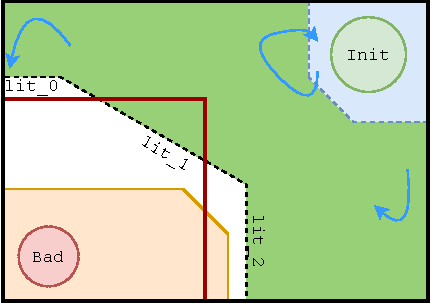
\includegraphics[width=0.99\textwidth]{figures/doping-lemma.pdf}
    \caption{An inductive lemma L = \{\texttt{lit\_0}, \texttt{lit\_1}, \texttt{lit\_2}\}}
    \label{fig:lemma}
	\end{subfigure}
	\begin{subfigure}[b]{0.3\textwidth}
    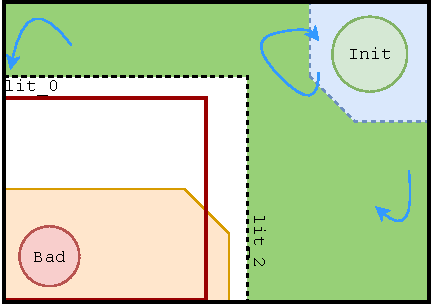
\includegraphics[width=0.99\textwidth]{figures/doping-lemma_gen.pdf}
    \caption{L is successfully generalized by dropping \texttt{lit\_1}}
    \label{fig:ind_gen}
	\end{subfigure}
	\begin{subfigure}[b]{0.3\textwidth}
    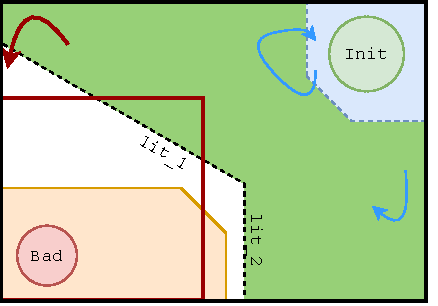
\includegraphics[width=0.99\textwidth]{figures/doping-lemma_not_ind.pdf}
    \caption{L no longer inductive by dropping \texttt{lit\_0}}
    \label{fig:not_ind_gen}
	\end{subfigure}

  \caption{Visualization of inductive generalization.}
  \label{fig:vis_ind_gen}
\end{figure*}




\paragraph{IC3/PDR.}
blah

\emph{Inductive generalization} 
A lemma $L$ over-approximates the reachable states from $\Init$, illustrated as the green region in \cref{fig:lemma}. $L$ is \textit{inductive relative to a context} $F$ iff given that $F$ is satisfied, from anywhere in the green region, after one step of the transition system, we are still in the green region (illustrated by the blue arrows). From IC3/PDR's standpoint, a lemma is represented as a set $\cS$ of constraints (literals), and its goal is to find a subset $\cS'$ that is still inductive relative to the same $F$. As we can see from \cref{fig:not_ind_gen}, starting from the lemma $\{\texttt{lit\_0}, \texttt{lit\_1}, \texttt{lit\_2}\}$, dropping \texttt{lit\_0} results in a lemma that is no longer inductive, while dropping \texttt{lit\_1} doesn't affect its inductiveness, as illustrated in \cref{fig:ind_gen}.

% \spc maintains the following data structures:
% \begin{itemize}
%     \item A unrolling depth $N$
%     \item An under-approximation $U$ of reachable states
%     \item  A queue of \emph{proof obligations} $Q$, where each proof obligation (\pob) in $Q$ is a pair $\langle \varphi, i \rangle$ of a cube $\varphi$ and a level number $i$, $0 \leq i \leq N$. Each POB is a region containing a potential counterexample that we want to prove to be unreachable (blocked) in $i$ steps.
%     \item A trace of frames $\cO$, in which each frame $\cO_i$ is a set of lemmas. Intuitively, each frame $\cO_i$ over-approximates states reachable up to $i$ steps from $\Init$. A lemma is learnt when a POB is blocked. Intuitively, a lemma is a region containing the reachable states but not the POB (the green region if Fig \ref{fig:ind_gen}, 
% \end{itemize}
% At the high level, the main IC3/\spc loop will try to find a counterexample of length $N$, and terminate if the counterexample is found (UNSAFE), or the lemma that proves such counterexample doesn't exist is a safe inductive invariant(SAFE). 

% The \texttt{Candidate} rule adds an initial \pob $\langle \Bad, N \rangle$ to
% the queue. If a \pob $\langle \varphi, i \rangle$ cannot be blocked because
% $\varphi$ is reachable from frame $(i-1)$, the \texttt{Predecessor} rule
% generates a predecessor $\psi$ of $\varphi$ using MBP and adds $\langle \psi,
% i-1 \rangle$ to $Q$. The \texttt{Successor} rule updates the set of reachable
% states if the \pob is reachable. If the \pob is blocked, the \texttt{Conflict}
% rule strengthens the trace $\cO$ by using interpolation to learn a new lemma
% $\ell$ that blocks the \pob, i.e., $\ell$ implies $\neg \varphi$. The
% \texttt{Induction} rule strengthens a lemma by inductive generalization and the
% \texttt{Propagate} rule pushes a lemma to a higher frame. If the $\Bad$ state
% has been blocked at $N$, the \texttt{Unfold} rule increments the depth of
% unrolling $N$. In practice, the rules are scheduled to ensure progress towards
% finding a counterexample.\DecMargin{0.1in}




% The main IC3/\spc loop will try to find a counterexample of length $N$, and terminate if the counterexample is found (UNSAFE), or the lemma that proves such counterexample doesn't exist is a safe inductive invariant(SAFE). 

% The main data structure in \spc is a queue of proof obligation $Q$, and 

% \cref{alg:spc} presents the key ingredients of \Spacer as a set of guarded
% commands (or rules). It maintains the following. Current unrolling depth $N$ at
% which a counterexample is searched (there are no counterexamples with depth less
% than $N$). A \emph{trace} $\cO = (\cO_0, \cO_1, \ldots)$ of \emph{frames}, such that
% each frame $\cO_i$ is a set of \emph{lemmas}, and each lemma $\ell \in \cO_i$ is
% a clause.
%  A queue of \emph{proof obligations} $Q$, where each proof obligation
% (\pob) in $Q$ is a pair $\langle \varphi, i \rangle$ of a cube $\varphi$ and a
% level number $i$, $0 \leq i \leq N$. An under-approximation $\cU$ of reachable
% states. Intuitively, each frame $\cO_i$ is a candidate inductive invariant s.t.
% $\cO_i$ over-approximates states reachable up to $i$ steps from $\Init$.
% The latter is ensured since $\cO_0 = \Init$, the trace is monotone, i.e.,
% $\cO_{i+1} \subseteq \cO_i$, and each frame is inductive \emph{relative} to its previous one,
% i.e., $\cO_i \wedge \Tr \limp \cO_{i+1}'$.
% Each \pob $\langle \varphi, i \rangle$ in $Q$ corresponds to a suffix of a potential
% counterexample that has to be blocked in $\cO_i$, i.e., has to be proven unreachable in $i$ steps.



% The \texttt{Candidate} rule adds an initial \pob $\langle \Bad, N \rangle$ to
% the queue. If a \pob $\langle \varphi, i \rangle$ cannot be blocked because
% $\varphi$ is reachable from frame $(i-1)$, the \texttt{Predecessor} rule
% generates a predecessor $\psi$ of $\varphi$ using MBP and adds $\langle \psi,
% i-1 \rangle$ to $Q$. The \texttt{Successor} rule updates the set of reachable
% states if the \pob is reachable. If the \pob is blocked, the \texttt{Conflict}
% rule strengthens the trace $\cO$ by using interpolation to learn a new lemma
% $\ell$ that blocks the \pob, i.e., $\ell$ implies $\neg \varphi$. The
% \texttt{Induction} rule strengthens a lemma by inductive generalization and the
% \texttt{Propagate} rule pushes a lemma to a higher frame. If the $\Bad$ state
% has been blocked at $N$, the \texttt{Unfold} rule increments the depth of
% unrolling $N$. In practice, the rules are scheduled to ensure progress towards
% finding a counterexample.\DecMargin{0.1in}


 


% Given a lemma in cube form $\cC$, its semantic meaning is that the system is safe at some state $\cS$ because of $\cC$. By dropping some of the literals in $\cC$, we ... 
% \nl{remember to add an example}

% The loop invariant is built within the given context of program. Thus it is natural to encode the program
% as an external memory module. However, in contrast to traditional memory networks [19, 20], where
% the memory slots are organized as a linear array, the information contained in a program has rich
% structure. A chain LSTM over program tokens can in principle capture such information but it is
% challenging for neural networks to understand with limited data. Inspired by Allamanis et al. [21], we
% instead use a graph-structured memory representation. Such a representation allows to capture rich
% semantic knowledge about the program such as its control-flow and data-flow

%%% Local Variables:
%%% mode: latex
%%% TeX-master: "0.0_main"
%%% End:

\section{Software debloating}
This section present needed domain background for \cref{chap:doccam}, which is software debloating using partial evaluation.
\paragraph{The software debloating problem.} Given a problem $\cP$ that has a set of functionalities $F = \{F_0, F_1, \dots, F_N\}$ and a user-specified subset of necessary functionalities $F_{spec} = \{F_i, F_j, \dots, F_k\}$, the goal of a software debloater is to produce a new program $\cP'$ that retains $F_{spec}$ and \emph{gracefully} refuses any functionalities in $F \setminus F_{spec}$.
\begin{figure}[t]
\begin{lstlisting}[language=Python]
parser = argparse.ArgumentParser()
parser.add_argument('-P', '--p-model-path', 
                    help='path to the .pt file of the model')
parser.add_argument('-F', '--fallback-mode', action='store_true', 
                    help='whether to run in fallback mode')
args = parser.parse_args()
def main():
    fallback_mode = args.fallback_mode
    
    if fallback_mode:
        server_config={
            "p_model": None,
            "fallback_mode": args.fallback_mode
        }
    else:
        p_model = setup_model(args.p_model_path)
        server_config={
            "p_model": p_model,
            "fallback_mode": args.fallback_mode
        }
        
    serve(server_config)
main()
\end{lstlisting}
    \caption{A bloated server \texttt{server.py}.}
    \label{fig:bloated_exp}
\end{figure}

\begin{figure}
    \begin{lstlisting}[language=Python]
{
    "main" : "server.py",
    "args" : ["-F"]
}
    \end{lstlisting}
    \caption{A specification file \texttt{spec.json} for \texttt{server.py}.}
    \label{fig:server_spec}
\end{figure}

\begin{figure}[t]
\begin{lstlisting}[language=Python]
parser = argparse.ArgumentParser()
parser.add_argument('-P', '--p-model-path', 
                    help='path to the .pt file of the model')
parser.add_argument('-F', '--fallback-mode', action='store_true', 
                    help='whether to run in fallback mode')
args = parser.parse_args()
def main():
    '''
    The original code for main
    '''
    ...

def main_specialized():
    fallback_mode = True
    server_config={
        "p_model": None,
        "fallback_mode": True
    }
    serve(server_config)
main_specialized()
\end{lstlisting}
    \caption{A debloated version of \texttt{server.py} with respect to \texttt{spec.json}.}
    \label{fig:software_debloated_exp}
\end{figure}
The Python server in \cref{fig:bloated_exp} has two modes: a fallback mode that doesn't require a trained neural network, and a normal mode that requires one. Given the specification in \cref{fig:server_spec}, in which user requires only the first functionality, one possible debloated version of the server is given in \cref{fig:software_debloated_exp}. Note that even though line 19 to 24 in \cref{fig:bloated_exp} are still in \cref{fig:software_debloated_exp}, it cannot be triggered, because the \texttt{main} function is not called. Remember that according to our problem definition, a debloated program is only about reducing functionalities, and the code itself could actually be more ``bloated''.

There are many ways to achieve the debloating goal, such as source-code optimization \cite{chisel}, binary optimization \cite{trimmer}, or compile-time optimization \cite{occam}. In this thesis, our focus is compile-time optimization, inspired by \occam \cite{occam}. Specifically, \occam's partial evaluator.

\paragraph{Partial evaluator.}
A \emph{partial evaluator} takes a program and some of its input values and produces a \emph{specialized} program in which those inputs are replaced with their values. In \cref{fig:software_debloated_exp}, \texttt{main\_specialized} is that specialized version of \texttt{main}.



%
% AG: not sure why soundness is important at this point of intro
% A sound partial evaluator must ensure that running the residual program on the
% remaining inputs always produces the same result as running the original
% program on all of its inputs.
%
While PE has been extensively applied to functional and logic programs, it was
less successful on imperative C/\cpp programs (with a notable exception of
\cmix~\cite{Andersen94} and \tempo~\cite{Consel98}). With the advent of
\llvm~\cite{llvm}, several new partial evaluators of LLVM bitcode have arisen
during the last few years (e.g., \llpe~\cite{llpe}, \occam~\cite{occam}, and
\trimmer~\cite{trimmer}). These tools leverage LLVM optimizations such as
constant propagation, function inlining, and others to either reduce the size of
the residual program (e.g., \occam and \trimmer) or improve performance (e.g.,
\llpe).

The key step of a PE-based debloater is to estimate whether specializing a function will result in a smaller (or more secure) final binary or library.
%Unfortunately, as with most problems in program analysis, this is very difficult.
As we can see in \cref{fig:software_debloated_exp}, specialization naturally increases the size of the code since it adds extra copies of functions into the code. However, since some inputs in the new functions have been replaced by constant values, optimizations such as constant propagation, might become enabled and result in new optimization opportunities in subsequent optimization passes. Therefore, the decision whether or not a function should be specialized for a particular call-site is non-trivial.
\section{Deep learning}
This section introduces deep neural networks, recurrent neural networks, and
reinforcement learning. They are the machine learning tools that we use in
\cref{chap:dopey} and \cref{chap:doccam}.
\begin{figure*}[t]
  \centering
  \begin{subfigure}[t]{0.3\textwidth}
    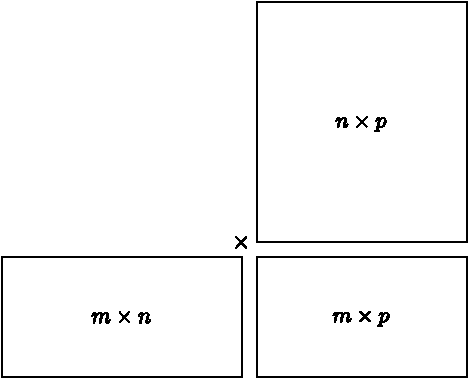
\includegraphics[width=0.99\textwidth]{figures/matmul.pdf}
    \caption{Matrix multiplication.}
    \label{fig:matmul}
	\end{subfigure}
	\begin{subfigure}[t]{0.3\textwidth}
    \adjincludegraphics[width=0.99\textwidth, trim={0 {.08\height} 0 0},clip]{figures/perceptron.pdf}
    \caption{Perceptron}
    \label{fig:perceptron}
	\end{subfigure}
	\begin{subfigure}[b]{0.6\textwidth}
    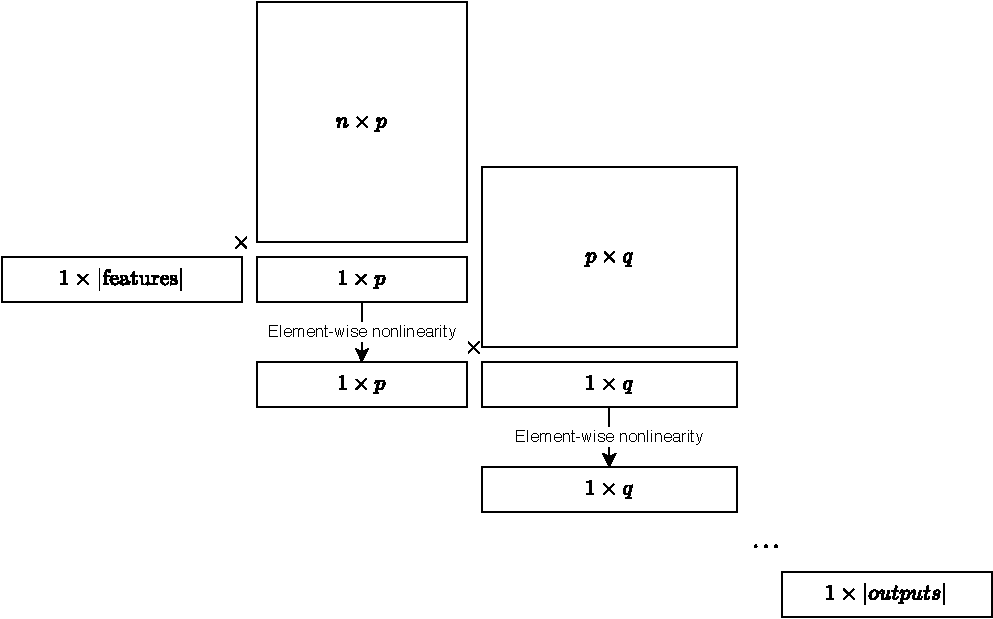
\includegraphics[width=0.99\textwidth]{figures/deep_matmul.pdf}
    \caption{Multi-layer Perceptron}
    \label{fig:deep_matmul}
	\end{subfigure}
	\begin{subfigure}[b]{0.6\textwidth}
    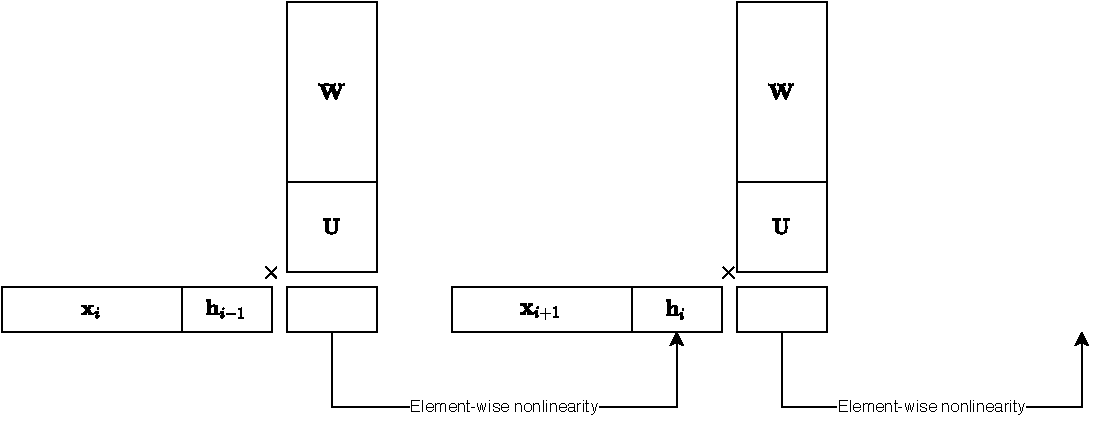
\includegraphics[width=0.99\textwidth]{figures/RNN.pdf}
    \caption{Recurrent neural network}
    \label{fig:rnn}
	\end{subfigure}  \caption{Visualization of matrix multiplication, perceptron,
    multi-layer perceptron, and recurrent neural network.}
\end{figure*}
\subsection{Perceptron. Multi-layer Perceptron. The fixed-size computing paradigm.}
There are already too many technical texts about the mathematical behind
Perceptron and Multi-layer Perceptron. In this section, we will take a pictorial
look at it, starting from matrix multiplication. Multiplying two matrices of
size $m \times n$ and $n \times p$ could be visualized as in \cref{fig:matmul},
which resulted in a new matrix of size $m \times p$.

\paragraph{Perceptron} is defined as a function that maps its input $\vect{x}$
(a real-valued vector) to an output value $y$ (a single binary value). While
there are many ways to define the mapping, in practice the perceptron function is
\begin{align*}
  y =  \twopartdef { 1 } {\vect{x} \times \vect{W} + \text{bias} > 0} 
                   { 0 } {\text{otherwise}}
\end{align*}
\cref{fig:perceptron} visualizes the perceptron function. In case of having to
classify $k$ classes ($k>2$), a one-vs-all scheme is used: learn $k$ separated
perceptron, each perceptron $p_i$ predicts whether $\vect(x)$ is of the class
$i^{th}$.

In the early 60s, it is believed that Single-layer perceptron was all we needed to learn
(approximate) any function. In 1969, Minsky and Papert \cite{perceptrons} proved
that a single perceptron cannot learn the simple XOR function, since XOR is not
\emph{linear separable}. There work effectively froze AI research for about ten years.

The solution for the XOR function, as it turned out, was very simple:
Multi-layer Perceptrons.

\paragraph{Multi-layer Perceptron.} To understand Multi-layer Perceptron, let's
take a step back and look at what a Single-layer Perceptron does: it computes a linear
transformation of the input ($\vect{x} \times \vect{W} + \text{bias}$), then
applies a non-linear filter (activation function) over the results (a branching function). The key
insight is that the result is also a matrix, hence can be feed into another
perceptron, which in total, make a non-linear function! In fact, it is proven \cite{universal}
that under certain assumptions, 2 layer perceptrons is enough to approximate arbitrary
functions!

\cref{fig:deep_matmul} visualizes a multi-layer perceptron. Looking at the
figure, it is also clear why it is also called \emph{Deep learning}. One way to
think about Deep learning, is that given a dataset $\cD$ of pairs $(\vect{x}_i, y_i)$, what
is a good architecture (the arrangement of intermediate matrices), and what are
the values for entries in the matrices.

\paragraph{The fixed-size computing paradigm.} Multi-layer perceptrons are
great, and could be used to approximate many functions. But it also forces
things to be in the same shape: once the architecture is fixed, all the matrices
in between are also fixed in shape, so all inputs have to have the same shape,
and all outputs also have to have the same shape as well. For many cases, this
is not a big problem: image could be resized into a fixed size, missing
values in an input vector could always be set to a dummy values, for examples.
But in some cases, the whole paradigm just doesn't work, and requires a
different paradigm altogether. 


\subsection{Recurrent-neural network. Tree LSTM.}
In many tasks, we need to process inputs of arbitrary length, to predict outputs also of arbitrary length (often called \emph{sequence-to-sequence} problems). There are multiple ways to make sequential inputs to work in the fixed-size paradigm, such as \emph{padding} (add dummy values to the inputs to make sure they are all of the same length), \emph{same length batching} (sort inputs by size and process inputs of the same size together), among others. However, those approaches doesn't help with handling sequential outputs. A better approach is \emph{recurrent neural networks} (RNNs). An RNN defines a function
\begin{align}
\vect{h}^t = f(\vect{h}^{t-1}, \vect{x}^{t})
\end{align}
in which $f$ is our linear transformation, followed by a non-linear filter. A
typical RNN can be
\begin{align}
  f(\vect{h}^{t-1}, \vect{x}^t) = tanh(\vect{x}_t \times \vect{W} + \vect{h}_{t-1} \times \vect{U} )
\end{align}
This simple RNN is visualized in \cref{fig:rnn}. Note that $\vect{W}$ and
$\vect{U}$ are shared. This also means that the longer the chain, the easier it
is for the first input to vanish/explode in the computation of the current
input, since $\vect{h}_t$ will have the term $\vect{x}_0\times\vect{W}^t$ in it.
In practice, vanilla RNNs rarely can learn for chains longer than 10 time steps.

To address this issue, a forget/gating mechanism is added to RNN, most notably
in architecture like LSTM \cite{lstm} and GRU \cite{gru}. Equations to compute
the output (update) at the time step $t$  for LSTM
with a forget gate are:
\begin{align}
  \vf_t &= \sigma(\vect{x}_t \times \vect{W}_f + \vect{h}_{t-1} \times \vect{U}_f + \text{bias}_f)\\
  \vi_t &= \sigma(\vect{x}_t \times \vect{W}_i + \vect{h}_{t-1} \times \vect{U}_i + \text{bias}_i)\\
  \vo_t &= \sigma(\vect{x}_t \times \vect{W}_o + \vect{h}_{t-1} \times \vect{U}_o + \text{bias}_o)\\
  \va_t &= \tanh{(\vect{x}_t \times \vect{W}_a + \vect{h}_{t-1} \times \vect{U}_a + \text{bias}_a)}\\
  \vc_t &= \vf_t \circ \vc_{t-1} + \vi_t \circ \va_t \\
  \vh_t &= \vo_t \circ \tanh{(\vc_t)}
\end{align}
where $\sigma$ is the sigmoid activation function, and $\circ$ is the
element-wise product.

\paragraph{TreeLSTM}
While LSTM works well on a sequence of inputs, it doesn't explicitly work with a
tree of inputs, such as an Abstract Syntax Tree (AST). One can force LSTM to work with a tree like of inputs by
flattening the tree into a sequence of tokens, but this normally requires adding
more separator tokens (like brackets) into the sequence, making if inefficient.
A better way is to directly enforce the tree structure into the update
equations, which was introduced in \cite{TreeLSTM}. Given a tree, let $C^j$
denote the set of children of node $j$. The Child-Sum TreeLSTM update equations
are:
\begin{align}
  \vs_j &= \sum_{k\in C^j}{\vh_k} \label{eq:summation}\\
  \vf_{jk} &= \sigma(\vect{x}_j \times \vect{W}_f + \vect{h}_{k} \times \vect{U}_f + \text{bias}_f)\\
  \vi_j &= \sigma(\vect{x}_j \times \vect{W}_i + \vect{s}_{j} \times \vect{U}_i + \text{bias}_i)\label{eq:tree-lstm-update-i}\\
  \vo_j &= \sigma(\vect{x}_j \times \vect{W}_o + \vect{s}_{j} \times \vect{U}_o + \text{bias}_o)\label{eq:tree-lstm-update-o}\\
  \va_j &= \tanh{(\vect{x}_j \times \vect{W}_a + \vect{s}_{j} \times \vect{U}_a + \text{bias}_a)}\label{eq:tree-lstm-update-a}\\
  \vc_j &= \vi_j \circ \va_{j} + \sum_{k \in C^j}{\vf_{jk} \circ \vc_k} \\
  \vh_j &= \vo_j \circ \tanh{(\vc_j)}
\end{align}
Intuitively, TreeLSTM incorporates the \emph{summation} of outputs of children
(\cref{eq:summation}) into the computation of the parent node
(in \cref{eq:tree-lstm-update-i} to \cref{eq:tree-lstm-update-a}, TreeLSTM uses
$\vs$ instead of $\vh$ as in vanilla LSTM), which enforces the tree structure.
Note that TreeLSTM is a generalized version of vanilla LSTM: if each node has exactly one child, we get the same equations as in
vanilla LSTM.
%% Recurrent neural networks (RNNs) are widely used in natural language processingtasks, especially speech recognition and machine translation. The primary goal ofRNNs is to approximate the mapping from a sequence of inputsx(1),...,x(t)to eithera single outputyor a sequence of outputsy(1),...,y(t). An RNN defines a mappingh(t)=f(h(t−1),x(t);θ)(2.2)whereh(t)is the hidden state, from which the final outputy(t)can be computed byeither a non-linear transformation or an MLP.11
%% Popular RNN models.A simple RNN model can be. The key issue of such a simple form is that the long-termdependencies are hard to capture, which makes training extremely difficult. Toaddress this issue, a commonly used RNN model is the long short-term memorynetwork (LSTM) [89], which introduces amemory cell with various gatesto preservestate over a long sequence.LSTM maintains two states — the original hidden state and a newly introducedcontextstate (or memory cell). At a high level, LSTM defines a mapping functionas follows:h(t),c(t)=f(h(t−1),c(t−1),x(t);θ)(2.4)whereh(t)is the hidden state andc(t)is the context state. These two states areupdated by three gates — input gatei(t), forget gatef(t)and output gateo(t)asfollows:i(t)=σ(Wix(t)+Uih(t−1)+bi)f(t)=σ(Wfx(t)+Ufh(t−1)+bf)o(t)=σ(Wox(t)+Uoh(t−1)+bo)u(t)=tanh(Wux(t)+Uuh(t−1)+bu)c(t)=i(t)u(t)+f(t)c(t−1)h(t)=o(t)tanh(c(t))(2.5)whereθ=  [Wi,Ui,bi,Wf,Uf,bf,Wo,Uo,bo,Wu,Uu,bu],σis the sigmoid function,andis the element-wise product.Two common variants of LSTM are gated recurrent units (GRUs) [41] and tree-structured LSTM (Tree-LSTM) [177]. The former simplifies gates of LSTM for effi-ciency while the latter extends the modeling ability to tree structures.12

\subsection{Reinforcement learning}
% In many tasks, the learning goal is beyond predicting some predefined label for a given input. Instead, the learning goal is to reach some beneficial state after a se- quence of actions following a set of rules from some initial state. Thus, what is really learned is a policy, which predicts an action given a state and the action is ideally optimal towards the ultimate beneficial state. Reinforcement learning is a system- atic methodology of solving this exact problem and has achieved remarkable suc- cesses in many challenging problems, particularly games. Prominent examples are strategical games like Chess [93] and Go [166], and video games like Atari [124], StarCraft [179], and Dota [132].
In many tasks, a dataset of input-output pairs $(\vec{x}, y)$ is too expensive,
or even impossible to obtain: imagine having to label all the best moves for
half of the number of all possible chess boards! More importantly, in many
cases, we do not really need one single correct output, but many possible
outputs are equally good, as long as their cumulative effects are the same: as
long as we reach the destination in time, it doesn't really matter whether our
speed at time $t$ is 40 or 50 km/h. To solve those two problems, we need to have
a learning paradigm that optimizes for a global \emph{goal}, while collecting
the data all by itself. \emph{Reinforcement learning} is such a paradigm, and
has achieved remarkable successes in many difficult tasks, such as Robotics
\cite{convai} or playing board games \cite{td-gammon, alphago}.

\paragraph{Markov Decision Process.} A standard formulation of RL is using
Markov decision process (MDP):
\begin{itemize}
  \item A set of states $S$;
  \item a set of actions $A$;
  \item $P_a{s, s'} = Pr(s_{t+1} = s' \mid s_t = s, a_t = a)$ is the probability
    a state $s$ will transit to another state $s'$, by taking the action $a$;
  \item $R_a{s, s'}$ is the reward \emph{after} transition from $s$ to $s'$ by
    taking the action $a$.  
\end{itemize}
At each time step $t$, the system interacts with its environment and receives
the current state $s_t$ and the immediate reward $r_t$. The goal of RL is to
learn a policy $\pi: A \times S \mapsto [0, 1], \pi(a, s) = Pr(a_t=a|s_t=s)$
that defines the probability of taking an action $a$ when in state $s$. Note
that in this thesis, we only care about finite state spaces (discrete actions).
There is also continuous state spaces, i.e predicting the
optimal speed at each time step. We want $\pi$ to maximize the expected
cumulative reward. In our setting, where $P$ is deterministic (taking one action
will result in only one possible new state), the cumulative
reward is defined as:
\begin{align}
  E = \sum_{t=0}^{T-1}{R_{a_t}(s_t, s_{t+1})}
\end{align}
where $T$ could be $\infty$ if necessary.

The dilemma of RL lies in the fact that we often do not have access to the true
reward function $R$ (if we do, we can simply sample many tuple $(s, a,
R_a(s))$ and learn it in a supervised manner), only the final reward at the
end of the execution of the policy, but in practice RL cannot be trained without
intermediate feed backs. For example, imagine if we can only train a Chess RL agent if the
only reward is a binary signal at the end! Hence, a big part of RL research is
about crafting adequate \emph{proxy rewards}, that tells the agent how well
it currently performing. One can directly craft the proxies using domain
knowledge, such as assigning scores for board configurations in Chess, or use
best-so-far random policy as the target (e.g Policy Gradient \cite{reinforce}), or learn the reward
function for a state-action pair instead of the reward for just the state
(e.g Deep-Q learning \cite{deepq}).
% \section{gRPC}
\chapter{Learning Literal Co- and Anti-occurrences for Inductive Generalization}
\label{chap:dopey}
% \NL{remember to add number to show that inductive generalization is really slow in practice}

\section{Introduction}
\label{chap:intro}

Model checking has been widely used in various important areas such as robustness analysis of deep neural networks~\cite{Katz:cav19}, verification of hardware designs~\cite{SMC96}, software verification~\cite{Ball02}, analysis~\cite{ESC-java-02} and testing~\cite{Sheyner:SP02}, parameter synthesis in biology~\cite{Barnat:biology12}, and many others. 
The central challenge of model checking is to find a concise and sound approximation of all possible states a given system may reach, which does not cover any undesired states (i.e. violating given specifications). 
Tremendous processes have been made by innovations in efficient data representations~\cite{BDD}, scalable SAT solvers~\cite{CDCL,chaff,minisat}, and effective heuristics~\cite{CEGAR,BMC,McMillan:cav06}.  
Modern model checkers share a common basis, namely, IC3~\cite{IC3}, of which the key insight is \textit{inductive generalization (IG)}.
This idea has been generalized to support rich theories~\cite{GPDR} that are crucial for many verification tasks~\cite{Komuravelli:cav13,SeaHorn} beyond hardware verification. 
The generalized IC3 with rich theories, also known as satisfiability checking for Constrained Horn Clauses modulo Theory
(CHC)~\cite{DBLP:conf/birthday/BjornerGMR15}, becomes the core part of a broad range of verification tasks.


% \NL{essentially it is a search problem, and traditionally handcrafted heuristics are used. ML can give better heuristic blabh blah}
% With deep learning models being applied in many real life application, verifying them is very important, and push traditional model checking methods to its boundary.

Existing IG techniques follow either an enumerative search process \cite{IC3,Bradley:fmcad11} or ad-hoc heuristics \cite{Griggio:CAD16,GSpacer}. 
Heuristics are effective but may demand non-trivial domain-specific (or even problem-specific) expertise. 
In this work, we aim to automatically learn such heuristics from the past successful IGs. 
We observe that verification problems as well as associated IGs are not isolated from each other. 
Taking software verification as an example, verifying different properties of the same program involves similar or same IGs; different versions of programs have similar code base; and
different software may use same coding convention, idioms, library or framework, resulting in similar structures.


% Can inductive generalization heuristics be automatically learned?
Our approach is inspired by the recent advances in deep learning, which automatically learn non-trivial patterns from raw pixels~\cite{Krizhevsky:nips12} as well as semantic correlations between natural language texts~\cite{Mikolov:nips13}.
A natural solution is to train a deep learning model to directly perform IG. 
However, IG raises many new challenges for deep learning. 
% symbols, 
% structured data,
% semantic reasoning (semantic valid/correct), 
% soundness,
% training data.
First of all, the input and the output of IG are symbolic expressions, which are \textit{highly structured} with \textit{rich semantics}. 
Slight syntactic variations can lead to dramatic changes in semantics.
Second, more importantly, IG has to satisfy complicated \textit{semantic constraints}. 
Third, given deep learning models hardly provide any reliable guarantees, how to design a neuro-symbolic system that exhibits \textit{learnability} from past experiences but still preserves \textit{soundness}?
% Fourth, how to learn a neural model through a sequence of complicated logical reasoning which are clearly \textit{not differentiable}?
All these challenges have to be properly addressed in building a neuro-symbolic reasoning framework. 
In this work, we share our design choices and empirical findings in building a neuro-symbolic engine \dpy, which introduces a neural component into symbolic model checking. 
Specifically, we make the following contributions: 
\begin{itemize}
    % \item we study the performance bottleneck of symbolic model checking and
    % factor out a component that are suitable for learning from the past runs;
    \item we adapt standard deep learning models to effectively represent symbolic expressions by incorporating both syntactic and semantic information;
    \item we design a simple but effective learning objective so that training data can be collected with nearly no changes of existing model checkers; 
    \item our integration algorithm achieves the soundness by design, and in the worst case, the learning component may only hurt the running time performance; 
    \item we implement \dpy on top of \spc, a state-of-the-art CHC-solver, using an efficient client-server architecture;
    \item our empirical evaluations indicate \dpy significantly improves \spc on 
    challenging benchmarks from \chccomp.
\end{itemize}


\input{3-2-Background}
\section{Overview}
\label{sec:overview}
\begin{figure*}[t]
  \centering
  \begin{subfigure}[b]{0.4\textwidth}
  \centering
    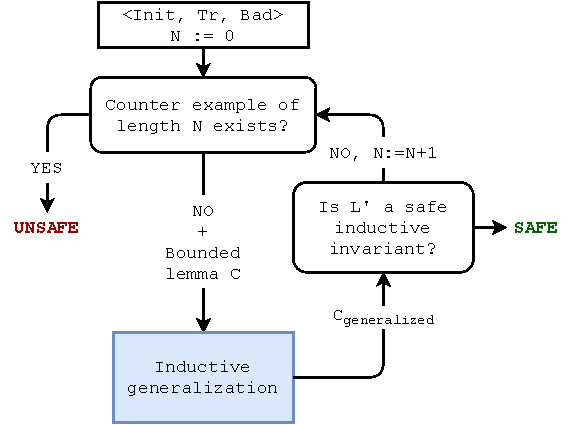
\includegraphics[height=4cm]{figures/doping-spacer}
    \caption{SMC architecture.}
    \label{fig:smc}
  \end{subfigure}
  \begin{subfigure}[b]{0.31\textwidth}
    \centering
    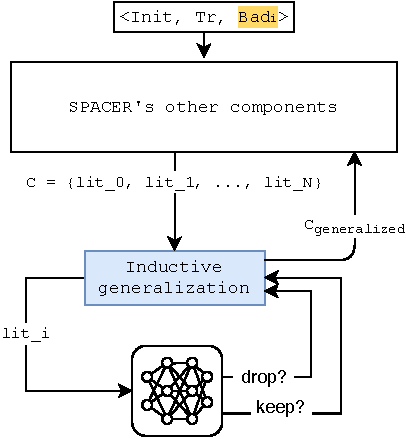
\includegraphics[height=4cm]{figures/doping-Page-general_architecture.pdf}
    \caption{\dpy architecture.}
    \label{fig:dopey}
	\end{subfigure}
  \begin{subfigure}[b]{0.15\textwidth}
  \centering
    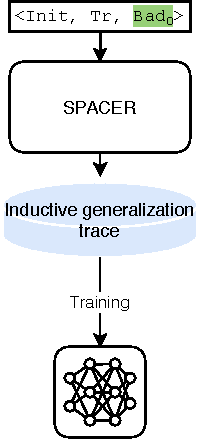
\includegraphics[height=4cm]{figures/doping-training.pdf}
    \caption{\dpy training.}
    \label{fig:spc_train}
	\end{subfigure}
	\caption{Overview of Symbolic Model Checking and overview of \dpy.}
  \label{fig:overview}
\end{figure*}
In this section, we give an overview of our technique, outline the challenges
involved, and our key insights to address them. The context is symbolic
SMT-based Model Checking (SMC)~\cite{IC3,GPDR,spacer}, also known as
satisfiability checking for Constrained Horn Clauses modulo Theory
(CHC)~\cite{DBLP:conf/birthday/BjornerGMR15}. In Model Checking, the high-level
goal is to show that an infinite state transition system ($Tr$) does not have an
execution/path that reaches a set of bad states ($\Bad$) by finding a formula
$\Inv$ that is an inductive invariant of $\Tr$ and does not intersect with
$\Bad$. The goal of CHC solving is to show that a set of First Order Logic
formulas $\Phi$ that satisfy the Horn
restriction~\cite{DBLP:conf/birthday/BjornerGMR15} is satisfiable by exhibiting
a symbolic formula $M$ that defines an FOL model that satisfies $\Phi$. The two
problems are closely related. Model Checking often reduced to CHC solving. Both
problems are in general undecidable.

\cref{fig:smc} shows the basic structure of an SMC algorithm based on IC3
architecture. In the paper, we use SMC \spc~\cite{spacer}, but the architecture is
common to many engines. SMC iteratively unrolls the $\Tr$, uses an SMT solver to
find a bounded counterexamples (which is usually decidable), and, if no
counterexample is found, attempts to create an inductive invariant. The
invariant is constructed as a set of so called \emph{lemmas}, where each lemma
is disjunction of atomic formulas. An example lemma is $x \leq 0 \lor y > 0$.
For convenience, we often represent lemmas as a set of formulas, writing instead
$\{x \leq 0,y > 0\}$. Many of the details of the algorithm are not important,
and we omit them here. The step we focus on in this paper is \emph{inductive
  generalization} (highlighted in blue in \cref{fig:smc}), that is responsible
for generalizing learned lemmas. In practice, this step is crucial for the
performance of SMC.

Conceptually, inductive generalization is a simple process, usually done with an
algorithm similar to the one we call \textsc{IterDrop}, shown in
\cref{alg:iter_drop}. \textsc{IterDrop} starts with a valid lemma $\ell = \{l_1,
\ldots, l_n\}$, and proceeds to generalize $\ell$ by removing an arbitrary
chosen literal from $\ell$, and using an SMT solver to check whether the lemma
is still valid (by calling \texttt{isInductive}). 
The details of \texttt{isInductive} are not important -- but it can be quite expensive. If the call succeeds, the literal is removed, otherwise it is kept. The goal is to generalize to a valid lemma with fewest literals.

From now on, when the context is clear, we use \emph{generalization} instead of inductive generalization.

% \setlength{\textfloatsep}{0pt}% Remove \textfloatsep
\begin{algorithm2e}[t]
\DontPrintSemicolon
\SetKwProg{Fn}{function}{}{end}

\SetKwFunction{Fdrop}{dropOne}
\SetKwFunction{Finductive}{isInductive}
\SetKwFunction{Fpick}{pick}


\KwIn{the original F-inductive lemma $L =\{l_1, l_2, ...,l_n\} $ }
\KwOut{a generalized F-inductive lemma $K \subseteq L $ }
$K \gets \emptyset $ \tcp*[l]{kept literals}  \label{line:spc-kept-lits}
$C \gets L $ \tcp*[l]{literals to check}

\While{$C \neq \emptyset  $}{
    $K,C \gets \Fdrop{K,C}$
}

\Return K
 
\vspace{4pt}

\Fn{\Fdrop{K, C}}{
    $lit \gets pick(C)$
    
    \uIf{ $\Finductive(K \cup\ C \setminus \{lit\})$} {
        $C \gets C \setminus \{lit\}$
    }
    \Else{
        $ K \gets K \cup \{lit\} $ ; %
        $C \gets C \setminus \{lit\}$
    }
    \Return $K, C$
}
\caption{\textsc{IterDrop} algorithm.}
\label{alg:iter_drop}
\end{algorithm2e}    

%%% Local Variables:
%%% mode: latex
%%% TeX-master: "../0.0_main"
%%% End:


We illustrate \textsc{IterDrop} with a sample run,  shown in
\cref{fig:spc_ind_gen}. \textsc{IterDrop} proceeds as follows:
\begin{itemize}
\item it tries to drop the first literal, $x_3 = \ltrue$, by checking whether
  $\ell'_1=\{x_1 = \ltrue, x_6 = 1, x_9 - x_{10} \geq 41, x_5 = 1\}$ is
  valid;
\item assume that $\ell'_1$ is valid, then $\ell \gets \ell'_1$, and $x_1 = \ltrue$ is chosen next;
\item now, assume that $\ell'_2 = \{x_6 = 1, x_9 - x_{10} \geq 41, x_5 = 1\}$ is
  not valid. $\ell$ remains as is and $x_6 = 1$ is chosen next;
\item assume that $\ell'_3 = \{ x_1 = \ltrue, x_9 - x_{10} \geq 41, x_5 = 1\}$ is valid, then
  $\ell \gets \ell'_3$, and $x_9 - x_{10} \geq 41$ is chosen next;
\item assume that $\ell'_4 = \{x_1 = \ltrue, x_5 = 1\}$ is not valid,
  then $\ell$ is unchanged, and $x_5 = 1$ is chosen next;
\item assume that $\ell'_5 = \{ x_1 = \ltrue, x_9 - x_{10} \geq 41\}$ is valid, then
  $\ell'_5$ is the final generalized lemma.
%   returned by \textsc{IterDrop}.
\end{itemize}
The example highlights the difficulty of inductive generalization. First, each
call to \texttt{checkInductive} is potentially very expensive. Thus, reducing
the number of the calls is highly desirable. Second, many of the calls, like
steps~2 and~4 are ``useless'' -- no new lemma is learned from them. Thus,
reducing such ``useless'' calls is also highly desirable. Finally, a solver
makes many (up to thousands) such inductive generalization calls per run.

\begin{figure*}[t]
    \centering
   \begin{subfigure}[b]{0.45\textwidth}
   \centering
        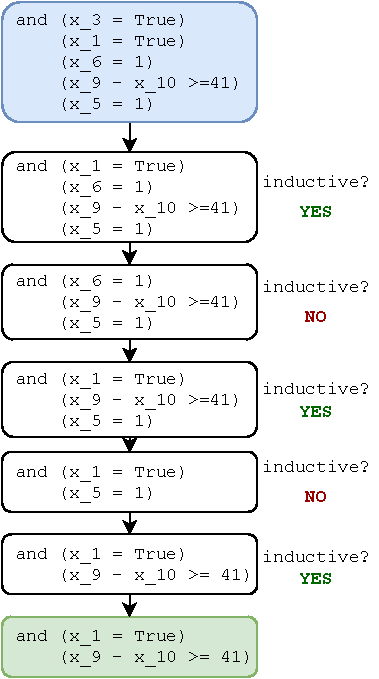
\includegraphics[width=0.8\textwidth]{figures/doping-spc_ind_gen.pdf}
        \caption{\textsc{IterDrop} example.}
    	\label{fig:spc_ind_gen}
	\end{subfigure}
    \begin{subfigure}[b]{0.45\textwidth}
    \centering
        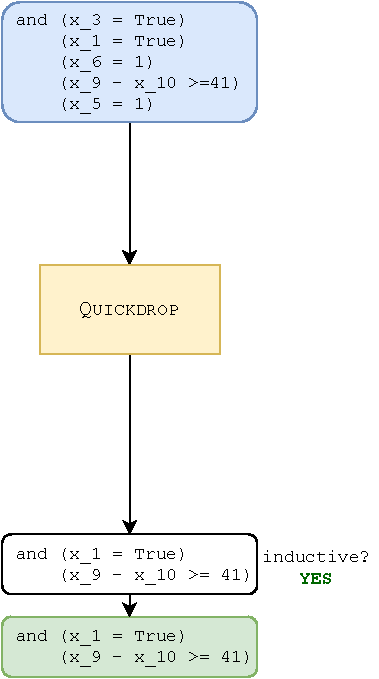
\includegraphics[width=0.8\textwidth]{figures/doping-spc_qd.pdf}
        \caption{\textsc{QuickDrop} example.}
    	\label{fig:spc_q_ind_gen}
	\end{subfigure}
	\caption{Examples of \textsc{IterDrop} and \textsc{QuickDrop}.}
    \label{fig:my_label}
\end{figure*}

\begin{figure*}[t]
    \centering
        \begin{subfigure}[b]{0.45\textwidth}
    \centering
        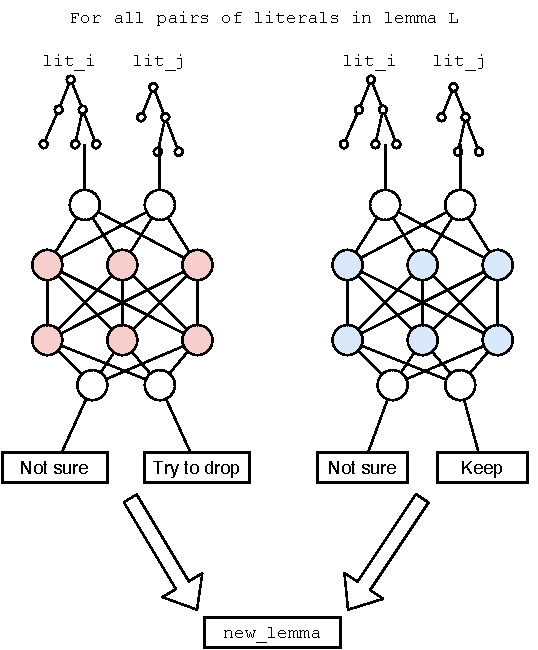
\includegraphics[width=0.8\textwidth]{figures/doping-model_vertical.pdf}
        \caption{\textsc{QuickDrop} example.}
    	\label{fig:spc_model_details}
	\end{subfigure}
	\begin{subfigure}[b]{0.45\textwidth}
	\centering
        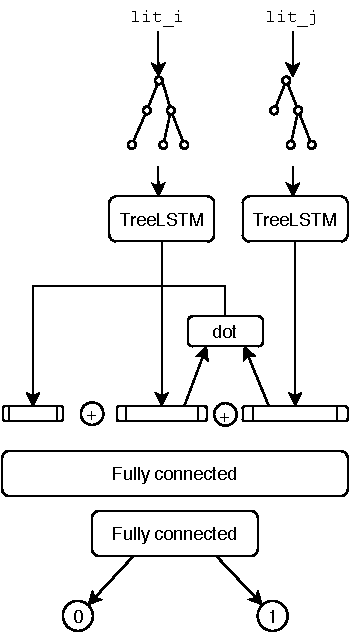
\includegraphics[width=0.6\textwidth]{figures/doping-model_detail.pdf}
        \caption{\textsc{QuickDrop} model.}
    	\label{subfig-4:model-detail}
	\end{subfigure}
    \caption{
      Architectures of \textsc{QuickDrop}.}
    \label{fig:architecture_of_qd}
\end{figure*}

Our \emph{key insight} is that since generalization happens
frequently, and, while the lemmas are different, the literals are similar, \emph{it is
possible to learn the co-occurrence between literals that do and do not occur in
the same lemma together}. We conjecture that once such a co-occurrence 
% (and anti-occurrence) 
is known, it can be used to guide \textsc{IterDrop} to make
fewer ``useless '' choices, and, ultimately, increase performance of SMC.
Furthermore, to avoid the difficulties of online learning, we rely on the fact
that many systems come with multiple properties (i.e., $\Bad$ states), and
learning from solving one property can be transferred to solving another.

Concretely, we propose a new SMC, called \dpy. As shown in
\cref{fig:dopey}, \dpy combines symbolic reasoning with guidance by a
neural network. The core of \dpy is a new neural-based generalization
algorithm called \textsc{QuickDrop}. Its pseudo-code is shown
in~\cref{alg:qdrop}. \textsc{QuickDrop} uses two neural networks, denoted by
$\Mpos$ and $\Mneg$, to predict whether a currently
chosen literal should be kept in the lemma or dropped. The prediction is based on past co- and anti-occurrences of pairs of  literals in lemmas. 

%Detailed description of \textsc{QuickDrop} is given in
%\cref{alg:qdrop}.

We illustrate a run of \textsc{QuickDrop} on the same example as
\textsc{IterDrop}. Recall that the initial lemma is $\ell = \{x_3 =
\ltrue, x_1 = \ltrue, x_6 = 1, x_9 - x_{10} \geq 41, x_5 = 1\}$.
% \ag{At this point, I do not understand the example. Please update it to be similar to the example for \textsc{IterDrop}.}
Assume that $x_1 = \ltrue$ is checked and kept, \tool proceeds as follows:
\begin{itemize}
\item it runs $\Mpos$ and predicts that $\{x_9 - x_{10} \geq 41\}$ should be kept;
\item it runs $\Mneg$ and predicts that $\{x_3 =
\ltrue, x_6 = 1\}$ should be dropped;
\item it combines the results from steps~1 and~2 and suggests a candidate $\ell_{cand}=\{x_1 =
  \ltrue, x_9 - x_{10} \geq 41\}$;
\item it checks the inductiveness of $\ell_{cand}$.
\end{itemize}
Note that \tool runs only \emph{one} inductiveness
check, compared to 5 used by \textsc{IterDrop}.
% (\cref{fig:spc_ind_gen}).

% \ag{I assume that example ends here}

% Given a lemma $\ell$, \dpy uses a neural component
% to predict which literals should be dropped and kept.


% \cref{fig:spc_train} shows how to train such component: we simply runs \spc to
% verify $\trs$, record the traces to a dataset, and use the dataset to train the
% neural component.

The key idea of \textsc{QuickDrop} is to use the \textit{co-occurrence} and
\textit{anti-occurrence} between literals in lemmas to predict which literals are
likely to be together in future lemmas. This intuition comes from an
observation that in many generalizations either: (a) a literal is
always got removed whenever another literal is kept (anti-occurrence) or (b) a
literal is kept whenever another literal is also kept (co-occurrence). We believe
that a) happens because the state space of a typical system under analysis can
be partitioned into disjoint components, and many lemmas reference only a few of
the components at a time; and b) happens because those literals are part of the same piece-wise linear function.

To learn the desired anti- and co-occurrence, we use two neural networks, called
$\Mneg$ and $\Mpos$, respectively. The networks are trained based on a run of an
SMC on a problem instance. We gather the set of all lemmas and their
generalizations, and use the data to train the network. Each network predicts,
given a literal $l_i$ the likelihood that a literal $l_j$ appears in a lemma
together with $l_i$. The details of the training are given in \cref{sec:learning-signal}.


% could be separated into disjoint areas, thus literals over variables
% in one area should be drop in a lemma over variables in a different area
% (antirelation). On the other hand, literals those together form a piecewise
% linear function that is used over and over should always stay together, since
% they are in fact parts of the same function (correlation). \ag{Parts of this
%   paragraph need to migrate to the insight above.}


%   \cref{fig:spc_train} shows how to train such component: we simply runs \spc to
%   verify $\trs$, record the traces to a dataset, and use the dataset to train the
%   neural component.

% \ag{This paragraph does not work. It is way too detailed for the overview.}
% \textsc{QuickDrop} uses two separated neural networks $\Ppos$ and $\Pneg$ (shown
% in blue and red, respectively, in \cref{subfig-4:model}). Given a pair of
% literals $(l_i, l_j)$ such that $l_i$ is already kept, $\Pneg$ predicts whether
% $l_j$ should be dropped, and $\Ppos$ predicts whether it should be kept. The
% details are shown in \cref{alg:qdrop}, where the blue lines mark the key
% differences between \textsc{IterDrop} and \textsc{QuickDrop}. Instead of 
% checking one literal at a time, \textsc{QuickDrop} predicts whether to drop or keep a set of
% literals (lines 4--5). We also need to \textsc{seed} the 2 networks by calling
% line 1 to keep at least a literal.  Let's see how
% \tool works on the same example as \textsc{IterDrop}.

\paragraph{Challenges.}
To make \dpy a practical verification engine, we have to address challenges in
three aspects: (a) machine learning, (b) logical soundness, and (c) engineering. For
machine learning, the challenge is in representing symbolic expressions as
vectors, while maintaining their rich semantic structure to enable to learn and
generalize co-occurrences between them. For logical soundness, the challenge is to use the neural nets
in a way that guarantees the soundness of a verification engine.
For engineering, the challenge is to
integrate ML and symbolic components in an effective way.

\paragraph{Representation learning of symbolic formula.}
Unlike raw images or natural language text, for which there are standard deep
learning models including convolutional and recurrent neural networks, a literal
in a lemma is a symbolic formula, which is structured and meaning of which is
sensitive to small changes. Simply viewing a literal as a sequence of tokens, as
in NLP, fails to capture the subtle semantic differences between structurally
similar literals.
    
    
We incorporate both syntactic and semantic information of a literal into its
representation. Our approach views a literal as a directed acyclic graph (DAG),
which is post-processed from its abstract syntax tree (AST), and
then adapts TreeLSTM~\cite{TreeLSTM} to embed such a DAG structure. Our approach
also takes semantic level information into consideration so that specific
properties of values are respected. For instance, embedding of numerical
values should preserve their relative order and equality.
    

% AG: someone, please move to macros
\begin{figure}[t]
  \centering
  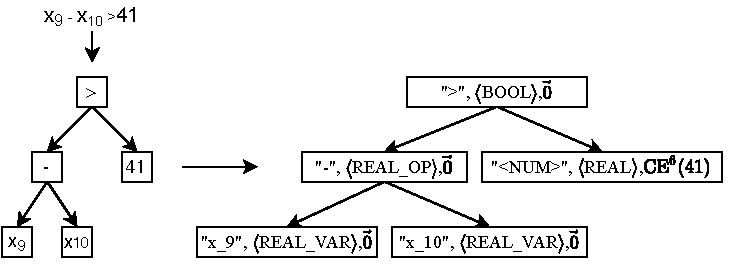
\includegraphics[width=0.8\textwidth]{figures/doping-ast-exp.pdf}
  \caption{An example of an AST and its semantic features.}
  \label{fig:ast_example}
\end{figure}

%%% Local Variables:
%%% mode: latex
%%% TeX-master: "0.0_main"
%%% End:


\paragraph{Learning for inductive generalization.}
Directly using machine learning to address the generalization problem
is a non-trivial structure prediction problem. It takes in a set of symbolic
formulas and outputs another set of symbolic formulas that are more
general and more concise. Though in principle, sequence-to-sequence
models~\cite{lample2019deep} are applicable, they are unlikely to accomplish such a
complicated reasoning task with existing ML models. In fact, even predicting
equivalence between two simple symbolic expressions remains
challenging~\cite{Allamanis:icml17}. Rather than having an end-to-end ML
solution, we embed a learning component in a classic symbolic approach of
generalization. Specifically, the learning component captures the
co-occurrence between literals appearing in past runs and predicts the likelihood
of keeping or dropping a literal in the current run.
Furthermore, uncertainties introduced by the learning component 
have to be carefully controlled, which otherwise could lead to
unsound conclusion. \dpy is designed to make sound progress no 
matter what predictions the learning component provides. Bad
predictions may be harmful to the performance, but not to soundness! 
   
    
\paragraph{Integrating machine learning with logical reasoning.}
ML models and logical reasoning framework are implemented in very different
programming environments and rely on different hardware. Their
integration unavoidably involves communication overhead among different runtimes and
hardware. This may offset performance gains of fast prediction, posing a significant engineering challenge. 
%
%Furthermore, uncertainties introduced by the learning component 
%have to be carefully controlled, which otherwise could lead to
%unsound conclusion. \dpy is designed to make sound progress no 
%matter what predictions the learning component provides. Bad
%predictions may be harmful to the performance, but not to soundness! 

% In particular, \dpy uses a positive model and a negative model
% at the same time to achieve more reliable predictions.

% \paragraph{Evaluation of neuro-symbolic design.}
% A straightforward way of evaluating a new design is to measure the run time used
% on solving some instances. The shorter, the better. However, the intricate
% complexity of a logical reasoning framework like \spc makes such a simple
% measurement problematic. A random decision at a particular step leads the
% subsequent search or reasoning to a very different direction, which may boost
% the performance accidentally. On the other hand, longer run time does not
% necessarily indicate that the learning component has no or negative value.
% Because the performance gain of having a learning (or neuro) component can be
% counteracted by two factors: the subsequent actions assuring soundness, and the
% communication overhead between the neuro part and the symbolic part. Our
% evaluation first analyzes the effectiveness of the learning component with a
% number of different design choices in various application scenarios, and then
% measures the gain or overhead of each component in wallclock time and other
% metrics like number of queries and number of inductive generation iterations.
% \ag{I don't think current evaluation section address the issues in this
%   paragraph. If we do not address these issues, we should move it into
%   discussion after experimental results. Say that we only measure run time, but
%   that is not necessarily adequate and one of the limitations to address in the
%   future.}\NL{I agree. Also I prefer 3 challenges over 4 anw}
%%% Local Variables:
%%% mode: latex
%%% TeX-master: "0.0_main"
%%% End:

\section{Representation learning}
\newcommand{\treelstm}{\textsc{TreeLSTM}\xspace}
\newcommand{\R}{\mathbb{R}}
\label{chap:rep-learning}
\paragraph{Representing symbolic formulas.}
We represent logical formulas as Abstract Syntax Trees (ASTs): operators label nodes of the tree, operands are children, constants (boolean and numeric) and variables are leaves. 
An example of an AST is shown in \cref{fig:ast_example}.
% For example, an AST representation for formulas $x_4 = \ltrue$ and $x_9 - x_{10} \geq 41$ are shown in \Cref{fig:ast_example}.
% \xs{consider merging fig-4 and fig-5 into one, which should show: 1) a formula; 2) its AST; 3) embeddings; why don't we draw figure in the same way as we did in the overview?}

ASTs are natural representations of formulas that are traditionally used in parsing and compilers. They preserve the key structure of the formula, while hiding (or abstracting) unnecessary details such as white space, commas and parentheses. Alternative representations, for example, as a sequence of tokens, abstract too much of the structure of the formula, while highlighting unnecessary differences.

\begin{figure}
  \centering
  \begin{align*}
    \textbf{Token}  &::= \text{Var} \mid \term{NUM} \mid \text{Op}\\
    \text{Var} &::= \text{variable name}\\
    \text{Op} &::= + \mid - \mid < \mid \cdots\\
    % \langle \text{NUM} \rangle &::= \text{``NUM''}
                                   \textbf{Kind} &::= \term{BOOL\_OP} \mid \term{REAL\_OP} \mid \term{BOOL\_VAR} \\
    \textbf{CE}^{n}(p) &::= s\; d_1 \cdots d_{2n+1} \hspace{1.5cm} s \in \R, d_i \in \{0, 1\}
  \end{align*}
  \caption{Grammar for AST node features.}
  \label{fig:features}
\end{figure}


%%% Local Variables:
%%% mode: latex
%%% TeX-master: "0.0_main"
%%% End:


Nonetheless, multiple semantically equivalent formulas can be represented by different trees. For example, the formulas $x + y > 0$ and $y + x > 0$ are semantically equivalent, yet differ in the concrete syntax, \emph{and} have different ASTs. To mitigate this, we put each formula in a ``normal'' form by simplifying all expressions that we can (for example, rewriting $x + 0$ into $x$), and ordering all associative operators. While there are many ways to normalize formulas (while not achieving a true normal form), we adopt a simple heuristic by using a simplification engine of the SMT solver Z3 \cite{z3}.
The normalizer cannot handle deep semantic equivalences, such as normalizing $2/7 \cdot x_9 - 4/7 \cdot x_{10} \geq 0$ into $1/7\cdot x_9 - 2/7 \cdot x_{10} \geq 0$. However, we believe it is good enough for our setting.
% \ag{Bad example, Z3 simplifier will reduce polynomials in exactly the way shown, it will also reduce all fractions}

Note that semantically equivalent rewriting and normalization make our representations of symbolic formulas essentially \textit{directed acyclic graphs (DAGs) modulo semantic equivalence}, because semantically equivalent subtrees share the exact same embedding. Indeed, representations of symbolic formulas in our implementation are DAGs, although they are viewed as if they were trees by the embedding model. Without further notice, when we refer to a node in a tree, we actually mean its corresponding node in the DAG.

% \ag{This last paragraph is very weak. This sub-section also ends without much of a conclusion.}
We use TreeLSTM~\cite{TreeLSTM} to aggregate information at each node in the tree into a fixed-length vector before feeding it to our subsequent networks. The process is illustrated in \cref{subfig-4:model-detail}. In the rest of this section, we describe the features that are used to encode each AST node into a vector to be combined by a TreeLSTM.


\paragraph{AST node features.}
We assume that the reader is familiar with the basics of the TreeLSTM neural networks. One of the main requirements is that each node $N$ of the input tree must be represented by a fixed-length vector in $\R^n$.

A common technique to map a node $N$ to a vector is to first map the infinite (or simply large) set $\Sigma$ of all possible nodes into a finite set $T$ of tokens (a.k.a.  \emph{tokenization}), and then have a dictionary $E$ that maps each token in $T$ into a fixed-length vector (a.k.a. \emph{embedding}). During tokenization, many nodes have to be mapped into the same token. For example, in NLP applications, all out-of-vocabulary words are mapped into a token \texttt{<UNK>}. Similarly in Programming Language applications, all variable and function names and all numeric constants are mapped into three tokens: \texttt{<VAR>}, \texttt{<FUNC>}, and \texttt{<NUM>}, respectively.

Unfortunately, this tokenization scheme is not applicable to our setting. We believe that both the variable names and the values of the numeric constants are highly relevant! For example, consider two pairs of formulas:
\begin{align}
   x_1 - 2x_{3} + 7x_{5} &\geq 10 & x_1 - 2x_{3} + 7x_{5} &\geq 14 \label{eq:pair_one}\\
   x_1 - 2x_{3} + 7x_{5} &\geq 10 & x_1 + x_{3} - x_{5} &\geq 0 \label{eq:pair_two}
\end{align}
Pair~\eqref{eq:pair_one} represents two parallel hyperplanes, with the first subsuming the second. Pair~\eqref{eq:pair_two} represents two intersecting hyperplanes and cannot be simplified any further. The difference between the two pairs disappears when all numeric constants are mapped to a small finite set of tokens. Yet, this difference is crucial for successful learning in our context! 




Instead, we represent each AST node by a vector of features that captures the necessary semantic information. Specifically, a node $N$ is first represented by a tuple $\langle\textbf{Token}, \textbf{Kind}, \textbf{CE} \rangle$. The grammar for each feature is shown in \cref{fig:features}, where angled brackets are used to represent terminals (e.g., $\term{\text{NUM}}$ is a symbol \texttt{<NUM>}). At the embedding step, \textbf{Token} and \textbf{Kind} are mapped into fixed-length vectors $\vect{T}$ and $\vect{K}$, while \textbf{CE} is \emph{not} embedded further. The final feature vector is the concatenation of $\vect{T}$, $\vect{K}$, and \textbf{CE}.

\textbf{Token} captures the symbol of the node. For variables and operations this is their syntactic representation; for real valued constants, it is a single token $\term{NUM}$. Note that each variable is kept as a \emph{separated} token. This is possible because in our setting, each system has finitely many variables.

\textbf{Kind} captures the type (or sort) of the expression rooted at the AST node. The value is one of a fixed pre-defined values such as $\term{\text{BOOL\_OP}}$, for a Boolean operator, etc. In principle, the sort can be learned automatically, similar to how heads in BERT~\cite{bert} seems to be able to learn part-of-speech for words in an unsupervised manner. However, we see no benefit of learning the sort since this information is already easily available.

\textbf{CE} (constant encoding) captures the numeric value of the node for real valued constants, and is a vector of $0$ for other nodes. The encoding of each number $p \in \R$ is parameterized by an encoding constant $n$ (in our experiments, $n = 6$) that determines the bounds of the magnitude of $p$.

Concretely, for each numerical constant $p$ that is represented as $s \times 10^{e}$ in the scientific notation, we encode the significant $s$ by its float representation and encode the exponent $e$ using a one-hot encoding vector. To one-hot encode $e$, we put $e$ in the range $[-n, n]$. If $e$ is out of range, we set it to either the upper or lower bound. For example, $\text{CE}^{2}(41) = [4.1 \, 0\, 0\, 0\, 1\, 0]$, and $\text{CE}^0(41) = [4.1 \, 1 ]$.  Our  motivation for $\text{CE}$ is to help \dpy to quickly extract  magnitudes of real constants along with their value.

We conclude this section with an example. \cref{fig:ast_example} shows an AST for $x_9 - x_{10} > 41$ and its transformation into a tree of feature vectors. The tree is further embedded and fed into a standard TreeLSTM model.
% The tree is further embedded and compressed into a DAG before being fed into a TreeLSTM.

% \ag{We talked about DAG in overview, but here the DAG has disappeared}


% % \begin{table}[]
% %     \centering
% %     \begin{tabular}{|p{1.8cm}|p{6cm}|}
% %         \hline
% %          Feature & Details  \\
% %          \hline
% %          \texttt{Token} & 

% %          \hline
% %          \texttt{Kind} & Each kind is the AST node's kind of a node, such as "BoolVar" (Boolean variable), "RealConst" (Real constant), etc.\\
% %          \hline
% %          \texttt{Constant Encoding} & A vector $\vect{C}$ of length $k$ encodes the real constant value. If the node is not a real constant, $\vect{C} = \vect{0} \in \R^{k}$\\
% %          \hline
% %     \end{tabular}
% %     \caption{}
% %     \label{tab:features}
% % \end{table}


% \begin{itemize}
%     \item \texttt{TOKEN}. Except for real constants, the token for each node is its string representation (\texttt{"x\_1"}, \texttt{"="}, etc). Note that each variable is kept as a \emph{separated} token: in our setting, each system has finitely many variables, hence a finite, and usually quite small, set of variable tokens suffices. Real constants are all mapped to the same \texttt{<NUM>} token.
%     \item \texttt{KIND}. We want our feature vector to preserve the kind (sort) of each token.
%     While this information in principle could be learned automatically in the
%     same vein that heads in BERT~\cite{bert} seems to be able to learn
%     part-of-speech for words in an unsupervised manner, we see no benefit of
%     learning it while we already have the precise kind information at hand.
% % This is because we learn on one $\trs$ and apply to the same
%   % $\trinit$ but with a different $\Bad$, so the set of variables stay the same
%   % between training and inferencing.
%     \item \texttt{Constant Encoding} 
%     We encode each real constant based on its scientific form: For each numerical constant $c = m \times 10^{n}$, we keep the coefficient $m$ and encode the exponent $n$ using a one-hot encoding vector. To one-hot encode $n$, we prefix a range for $n$, and if $n$ is out of range we set it to either the upper or lower bound. In this work, we bound $n$ by $[-6, 6]$, which is enough to contain all constants in our benchmark. 
  
% \end{itemize}
% \ag{Got stuck in number representation. This needs another passs. It should be possible to summarize the features in a table. Give mathematical definitions, like $|c|$ for magnitude, $\max(c_1, c_2)$ for maximum, etc. An example of tokenization is needed. The connection to transition relation and bad states seems out of place.}

% \ag{Need a name for our setting. The usual name is \emph{multi-property verification}. One system, many properties. Can cite recent FMCAD paper from Rozier et al. on that being an industrial problem. Then we learn on one property and transfer to other properties. Finding the right terms is to talk about what we do is super super important, don't just use any term, and once term is picked be very very consistent.}
% Moreover,  \ag{lost in this paragraph. Don't mix discussion and related work with main construction. First explain and illustrrate construction, then talk about birds and the bees.}
 % \dpy in Fig. \ref{fig:ast_example}, with the following feature vectors at each node:
% % we have the following feature vectors at the nodes:
% \begin{align*}
%     \Feat(x_9) &= [\texttt{"x\_9"}, \term{REAL\_VAR}, \vect{0}] \\
%     \Feat(x_{10}) &= [\texttt{"x\_10"}, \term{REAL\_VAR}, \vect{0}] \\
%     \Feat(-) &= [\texttt{"-"}, \term{REAL\_OP}, \vect{0}] \\
%     \Feat(>) &= [\texttt{">"}, \term{BOOL\_OP}, \vect{0}] \\
%     \Feat(41) &= [\texttt{"<NUM>"}, \term{REAL},\mathit{CE}^6(41)]
% \end{align*}
% in which $\mathit{CE}(41)$ is the constant encoding of $41$, as discussed in
% technique~\ref{trick2} \ag{The reference to the technique is unclear. Find a way
% to explain this differently}, $\texttt{NA} = \vect{0} \in \R^{|CE(41)|}$ is padding to make sure that all feature vectors are of the same length.
% with magnitude in the range $(10^{-1}, 10^1)$. \ag{This is first time that magnitude makes some sense, but I clearly had no clue what it was before}. The original and tokenized input trees are shown in \Cref{fig:embed_example}. \ag{Also use this example to illustrate an AST, instead of introducing new examples}. In the figure, 
% \texttt{NA} stands for a vector of the same length as the constant encoding, with all entries set to $0$ \ag{use math to be precise, introduce symbols, this should be $\texttt{NA} = \vect{0} \in \R^n$}. \ag{Use fonts to make figure readable}

% \ag{Figure uses tokens that have never been defined!}

% \begin{figure}[t]
% \Tree[.{'$\geq$', Bool, NA} [.{'-', Op, NA}   [{'x\_9', RVar, [0,0,0,0]} ]
%                     [.{'x\_10', RVar, NA} ]]
%               [.{'Num', RCon, [0,0,1,4.1]} ]]
% \caption{Example of an AST and its embedding.}
% \label{fig:embed_example}
% \end{figure}
% A design decision that works in symbolic representation learning has to face is how to tokenize real constants and variables: unlike mathematics operators, there are possibly an infinite number of real constants and variables. A common choice is to map all variables into a single token $\texttt{<VAR>}$, and all real constants into a single token \texttt{<NUM>} \cite{}, \cite{}.

% This mapping doesn't work in our case because.

% In this work, we propose to \emph{keep} each variable and real constant as a separated token. 
% \subsection{Generate training data}
% \paragraph{Correlation matrix}
% \paragraph{Antirelation matrix}
% Talk about why we encode our formulas this way: constant embedding, 
% \subsection{Model, loss function, training technique}
% Our literals are encoded as AST.

% TreeLSTM is a model that explicitly preserve information in a tree-structured topology. 

% The functions that we want to learn are not symmetric: f(l1, l2) != f(l2, l1). We explicitly enforce it by adding a dot product into the loss function

% Our matrices are sparsed: after capping, a majority of the entries in the matrices (> 90\%) are 0. To deal with it, we employ negative sampling technique: blah blah

% Those techniques are inspired by GloVe
% \subsection{Using the model}
% \texttt{initKeep} essentially is the same as \textsc{IterDrop}, but instead of running till the queue $\texttt{C}$ is empty, we run it till $\texttt{K}$ has at leask $k$ elements, in which $k$ is a parameter of our choosing.


% Given a Positive and a Negative model, we employ them following Algorithm
% \ref{alg:main}
%%% Local Variables:
%%% mode: latex
%%% TeX-master: "0.0_main"
%%% End:

\section{Learning co-occurrence probabilities}
\label{sec:learning-signal}
\newcommand{\thres}{\textit{threshold}}

% Directly using machine learning to address the inductive generalization problem is a non-trivial structure prediction problem, which takes a set of symbolic formulas as input and outputs another set of symbolic formulas that are more general and more concise.
%     Though in principle, sequence-to-sequence models \cite{seq2seq}
%     % machine learning models in NLP or machine translation 
%     are applicable, they are unlikely to accomplish such a complicated reasoning task with existing machine learning models. In fact, even predicting equivalence between two simple symbolic expressions remains challenging~\cite{Allamanis:icml17}.
%     Rather than having an end-to-end machine learning solution,
%     we embed a learning component in the classic symbolic approach of inductive generalization. 
%     Specifically, the learning component captures the co-occurrence between literals appearing in past runs and predicts the likelihood of keeping or dropping a literal in the current run. 

Recall from \cref{sec:overview} that in this work, instead of having an end-to-end ML solution, we learn to predict whether a literal could be dropped from a lemma, based on its co-occurrences with other literals in the training data. Concretely, we want to learn how likely a literal is kept, given the existence of another literal in the solution. While calculating the exact probability of this event in the training data and learn a neural network to approximate it in a \emph{regression} manner seems like a natural approach, it is actually not desirable: the exact probabilities, even with binning, \emph{are not consistent between different properties of the same system}. Fortunately, we observe that pairs with co-occurrence probabilities above a certain threshold are \emph{consistent} across different properties!

Thus, we frame our problem into a \emph{classification problem}:
% \xs{Insight and problem should be brought up earlier, rather than near the end}
\begin{problem}[Literal Co- and Anti-occurrence Classification]
% \label{prob:literal:rel}
Given a set of literals $\cL$ and a scoring function $f: \cL \times \cL \mapsto [0,1]$, 
train a classifier $M$ %$M : \cL \times \cL \mapsto [0,1] $ 
s.t. $M(\lit_i,\lit_j) \approx f(\lit_i, \lit_j)$.
\end{problem}
We use two scoring functions:
{\small\begin{align*}
    f^{+}(\lit_i, \lit_j) &=
    \twopartdef { 0 } {\Ppos_{ij} < \thres} 
                { 1 } {\Ppos_{ij} \geq \thres} \\
    f^{-}(\lit_i, \lit_j) &=
    \twopartdef { 0 } {\Pneg_{ij} < \thres} 
                { 1 } {\Pneg_{ij} \geq \thres}
\end{align*}}%
where $\Ppos$ and $\Pneg$ are co- and anti-occurrence matrices that capture the likelihood that two literals appear or do not appear in the same generalized lemma, respectively.
% \NL{We are still in the context of Problem 1, so }
To define $\Ppos$ and $\Pneg$ formally, assume that there is a a finite set of \emph{original} lemmas $\Lem$, and a corresponding  set of generalized lemmas $\GLem$. Inductive generalization is a function $\indgen: \Lem \mapsto \GLem$. The sets of all literals in $\GLem$ and $\Lem$ are $\GLit$ and $\Lit$, respectively. A generalized lemma is indicated by a prime, so that lemma $\ell'=\indgen(\ell)$ is the generalization of lemma $\ell$. Then, the co- and anti-occurrence matrices are defined as follows: 
{\small\begin{align*}
\Ppos_{ij} &= Pr(\lit_j \in \ell' \mid \lit_i \in \ell')\\
\Pneg_{i,j} &= Pr(\lit_j \not \in \ell' \mid \lit_i \in \ell', \lit_i \in \ell, \lit_j \in \ell)
\end{align*}}%
That is, $\Ppos_{ij}$ is the probability that a literal $\lit_j$ appears in a lemma $\ell' \in \GLem$ that contains $\lit_i$, and $\Pneg_{ij}$ is the probability that a literal $\lit_j$ does not appear in a lemma $\ell'$ given that literal $\lit_i \in \ell'$ and both $\lit_i$ and $\lit_j$ are in $\ell$. $\Ppos$ is of the size $|\GLit|\times|\GLit|$, and $\Pneg$ is of the size $|\Lit|\times|\Lit|$. They are \emph{not} complimentary: \mbox{$\Ppos_{ij} + \Pneg_{ij} \neq 1$}. Neither is symmetric: \mbox{$\Ppos_{ij} \neq \Ppos_{ji}$}~and~\mbox{$\Pneg_{ij} \neq \Pneg_{ji}$}.

% SAVE AND MOVE TO NHAM THESIS
% To define $\Ppos$ and $\Pneg$ formally, we begin with introducing some notation. Assume that there is a a finite set of \emph{original} lemmas $\Lem$, and a corresponding  set of generalized lemmas $\GLem$. Inductive generalization is a function $\indgen: \Lem \mapsto \GLem$. A generalized lemma is indicated by a prime, so that lemma $\ell'=\indgen(\ell)$ is the generalization of lemma $\ell$. Let $\Lit$ be the set of literals appearing in original lemmas, $\Lit = \{\lit\in \ell \mid \ell \in \Lem\}$; and $\GLit$ be the set of literals appearing in generalized lemmas, $\GLit = \{\lit\in\ell' \mid \ell' \in \GLem\}$.
\begin{itemize}
    \item Let $F$ be a literal-frequency matrix of size $|1\times\GLit|$. $F_i$ is the number of times a literal $\lit_i$ appears in a \emph{generalized} lemma.
    Formally, $F_i = |\{ \ell \in \GLem \mid \lit_i \in \ell\}|$.
    \item Let $X$ be a literal co-occurrence matrix of size $|\GLit| \times |\GLit|$. $X_{ij}$ is the number of times both $\lit_i$ and $\lit_j$ are in some \emph{generalized} lemma in $\GLem$. Formally, $X_{ij} = |\{ \ell \in \GLem \mid \lit_i \in \ell, \lit_j \in \ell\}|$.
    Note that $X_{ij} = X_{ji}$. For consistancy, we let $X_{ii} = F_{i}$.
    \item $\Ppos$ is a \emph{literal co-occurrence probability matrix} of size $|\GLit| \times |\GLit|$. $\Ppos_{ij}$ is the probability that $\lit_j$ appears in a \emph{generalized} lemma $\ell'$ given that $\lit_i$ is in $\ell'$. Formally, $\Ppos_{ij} = Pr(\lit_j \in \ell' \mid \lit_i \in \ell') = X_{ij}/F_i$ if $F_i \neq 0$, and $0$ otherwise. 
    
\end{itemize}

The definition of the anti-occurrence matrix $\Pneg$ is similar. \newcommand{\xcor}{X^\mathit{cor}}
\newcommand{\xanti}{X^{\mathit{anti}}}
\begin{itemize}
    \item Let $\xcor$ be a literal co-occurrence matrix of size $|\Lit| \times |\Lit|$, such that $\xcor_{ij}$ is the number of times $\lit_i$ and $\lit_j$ are in a lemma $\ell \in \Lem$. Formally, $\xcor_{ij} = |\{ \ell \in \Lem \mid \lit_i \in \ell, \lit_j \in \ell\}|$. Clearly, $\xcor_{ij} = \xcor_{ji}$.
    \item  Let $\xanti$ be a literal anti-occurrence matrix of size $|\Lit| \times |\Lit|$, such that $\xanti_{ij}$ is the number of times a pair $(\lit_i, \lit_j)$ satisfies the following conditions: (a) $\lit_i$ and $\lit_j$ are in in some lemma $\ell \in \Lem$, (b) $\lit_i$ is in the corresponding \emph{generalized} lemma $\ell' \in \GLem$, and (c) $lit_j$ is \emph{not} in $\ell'$. For consistancy, we set $\xanti_{ii} = 0$. Formally, $\xanti_{ij} = |\{ \ell \in \Lem 
    \mid 
    \ell' = indgen(\ell), 
    \lit_i,\lit_j \in \ell,  
    lit_i \in \ell', lit_j \not\in \ell'|\}$.
    \item     A literal anti-occurrence probability matrix $\Pneg$ of size $|\Lit| \times |\Lit|$ is defined such t hat $\Pneg_{ij}$ is the probability that $lit_j$ is \emph{not} the generalized lemma given that $lit_i$ is in the generalized lemma. Formally, $\Pneg_{ij} = \xanti_{ij}/\xcor_{ij}$ if $\xcor_{ij} \neq 0$, and $0$ otherwise. Note that, like $\Ppos$, $\Pneg$ is not symmetric.
\end{itemize}



     
    
% %    Note that $\Ppos_{ij} \neq \Ppos_{ji}$: the co-occurrence probability is \emph{not} symmetric.

% An an example, consider a set $\Lem = \{\ell_1, \ell_2, \ell_3\}$ of~3 original lemmas and the corresponding set $\GLem = \{\ell'_1, \ell'_2, \ell'_3\}$ of generalizations: 
% {\small\begin{align*}
%    \ell_1 &= \{\lit_1, \lit_2, \lit_3, \lit_4\} &  \ell'_1 &= \{\lit_1, \lit_2, \lit_3\} \\
%    \ell_2 &= \{\lit_1, \lit_2, \lit_3\} &  \ell'_2 &= \{\lit_1, \lit_2\} \\
%    \ell_3 &= \{\lit_1, \lit_3, \lit_4\} & \ell'_3 &= \{\lit_1\}
% \end{align*}}%
% % Then,
% % {\small\begin{align*}
% % \small
% % \Ppos &=
% %   \begin{vmatrix}
% %     1 & .67 & .33 \\
% %     1 & 1 & .5  \\
% %     1 & 1 & 1  \\
% %   \end{vmatrix} &
% %   \Pneg &= 
% %       \begin{vmatrix}
% %     0 & 0 & .67 & 1 \\
% %     0 & 0 & .5 & 1 \\
% %     0 & 0 & 0 & 1 \\
% %     0 & 0 & 0 & 0
% %   \end{vmatrix}
% % \end{align*}}%
% \NL{Fix the example}
% In the example:
% \begin{align*}
%     \Lem &=\{\ell_1, \ell_2, \ell_3\} & \GLem &=\{\ell_1', \ell_2', \ell_3'\}\\
%     \Lit &=\{\lit_1, \lit_2, \lit_3, \lit_4\} & \GLit &=\{\lit_1, \lit_2, \lit_3, \lit_4\}\\
%   F &= [3, 2, 1, 1] \\
%   X &= 
%   \begin{vmatrix}
%     3 & 2 & 1 & 1 \\
%     2 & 2 & 0 & 0 \\
%     1 & 0 & 1 & 0 \\
%     1 & 0 & 0 & 1
%     \end{vmatrix}
%     &
%   \Ppos &= 
%   \begin{vmatrix}
%     1 & .67 & .33 & .33 \\
%     1 & 1 & 0 & 0 \\
%     1 & 0 & 1 & 0 \\
%     1 & 0 & 0 & 1
%   \end{vmatrix}
% \end{align*}
% Thus, $\Ppos_{12} = 0.67$ and $\Ppos_{13} = 0.33$. That is,
 % $\lit_2$ is twice as likely as $\lit_3$ to be in the same generalized lemma as $\lit_1$.

%\newcommand{\xcor}{X^{\text{cor}}}
%\newcommand{\xanti}{X^{\text{anti}}}


\paragraph{Dataset creation and Model training.} Our goal is to learn the two classifiers $\Mpos$ and $\Mneg$ that approximate $f^{+}$ and $f^{-}$, respectively. To create the sets $\Lem$ and $\GLem$, we run \spc on an instance and collect all generalization steps. This data is used to compute $\Pneg$ and $\Ppos$ based on their definitions.
% \ag{This is where in the thesis the computation and definition of all the supporting matrices goes} 
We then fix a threshold and convert the matrices into a binary classification dataset.

% \xs{Remeber to have some paragraph titles; in this section so far, we have only one.}
We train both classifiers using the architecture shown in \cref{subfig-4:model-detail}. It consists of a TreeLSTM network followed by two fully connected layers. To enforce the asymmetry in the learned classifier, we take the dot product of the TreeLSTM output vectors and concatenate them together before feeding them to the first fully connected layer. Since both $\Ppos$ and $\Pneg$ are sparse, we employ a negative sampling rate, directly inspired by work on learning word co-occurrence probability~\cite{glove}.
% \xs{Why not end-to-end?}
% \NL{It is hard}

% \xs{Why two models?}
% \NL{Positive model tell you what literal to be kept, but for the other literals, it doesnt say whether a literal is more likely to be drop than another. Negative model explicitly tell you one literal is more likely to be dropped.}
% \xs{Let's have a paragraph motivating why we learn co-occurrence, instead of letting ML models be in charge of everything}
\paragraph{Discussion.} There are many alternative ways to guide generalization using a neural component than the one we chose. Perhaps most desirable is to have an end-to-end solution in which the neural component takes an original lemma as input and produces a generalized lemma as output. However,  the symbolic reasoning required for this is so complex that we believe that such a solution is much harder to train and scale up. Another alternative to learn an approximation of the inductive check, i.e., the function $\mathit{isInductive}(\mathit{Context}, \ell) \mapsto \{true, false\}$ that determines whether a candidate lemma $\ell$ is inductive in the current context. We have tried such an approach, but could not make it effective. The difficulty is that the $\mathit{Context}$ that is used by the inductive checker is a large symbolic formula. This makes training the network difficult. We suspect is as hard as \emph{learning a neural SMT-solver}~\cite{DBLP:conf/iclr/SelsamLBLMD19,DBLP:conf/sat/SelsamB19}. We have also considered using just the co- or anti-occurrence matrices, but the results are not as good as shown by our empirical evaluation (\cref{sec:dopey-exp}). 
% \ag{I don't see the difference between end-to-end and the second alternative}

% With the 2 learned models, we still need to address the issue of how to integrate them into \spc to do inductive generalization, which we will discuss in the following section.
%% THINGS TO APE
% 5PREDICTING SATISFIABILITY
%Although our ultimate goal is to solve SAT problems arising from a variety of domains, we beginby training NeuroSAT as a classifier to predict satisfiability onSR(40).  Problems inSR(40)aresmall enough to be solved efficiently by modern SAT solvers—a fact we rely on to generate the problems—but the classification problem is highly non-trivial from a machine learning perspective.Each problem has 40 variables and almost 200 clauses on average, and the positive and negativeexamples differ by negating only a single literal occurrence out of a thousand.  We were unable totrain an LSTM on a many-hot encoding of clauses (specialized to problems with 40 variables) topredict with>50% accuracy on its training set. Even the canonical SAT solver MiniSAT (Sorensson& Een, 2005) needs to backjump3almost ten times on average, and needs to perform over a hundredprimitive logical inferences (i.e.unit propagations) to solve each problem.
% We instantiated the NeuroSAT architecture described in§3 withd= 128dimensions for the literalembeddings, the clause embeddings, and all the hidden units;3hidden layers and a linear outputlayer for each of the MLPsLmsg,Cmsg, andLvote; and rectified linear units for all non-linearities.We regularized by the`2norm of the parameters scaled by10−10, and performedT= 26iterationsof message passing on every problem.  We trained our model using the ADAM optimizer (Kingma& Ba, 2014) with a learning rate of2×10−5, clipping the gradients by global norm with clippingratio0.65(Pascanu et al., 2012). We batched multiple problems together, with each batch containingup to 12,000 nodes (i.e.literals plus clauses). To accelerate the learning, we sampled the number ofvariablesnuniformly from between 10 and 40 during training (i.e.we trained onSR(U(10,40))),though we only evaluate onSR(40). We trained on millions of problems.After training, NeuroSAT is able to classify the test set correctly with 85% accuracy.  In the nextsection, we examine how NeuroSAT manages to do so and show how we can decode solutions tosatisfiable problems from its activations.  Note:  for the entire rest of the paper,NeuroSATrefers tothe specific trained model that has only been trained onSR(U(10,40))

%%% Local Variables:
%%% mode: latex
%%% TeX-master: "0.0_main"
%%% End:

\section{\dpy: \spc with \tool}
\label{sec:intergration}
\begin{algorithm2e}[t]
\DontPrintSemicolon
\SetKwProg{Fn}{function}{}{end}
\SetKwFunction{Fdrop}{dropOne}
\SetKwFunction{Finductive}{isInductive}

\SetKwFunction{Finit}{initKeep}
\SetKwFunction{Fdnnkeep}{$\Mpos$}
\SetKwFunction{Fdnndrop}{$\Mneg$}


\SetKw{Continue}{continue}  

\KwIn{the original F-inductive lemma $L =\{l_1,l_2,...,l_n\} $ }
\KwOut{a generalized F-inductive lemma $K \subseteq L $ }
$K \gets \textcolor{blue}{ \Finit{L}}$ \tcp*[l]{kept literals}  \label{line:def:kept-lits}

$C \gets L $ \tcp*[l]{literals to check}

\While{$C \neq \emptyset$}{
    \textcolor{blue}{
    $\Delta K \gets \{ l \ |\  l \in C  \wedge \Fdnnkeep(K, l) \} $
    } \label{line:deltaK}
    
    \textcolor{blue}{
    $\Delta C \gets \{ l \ |\ l \in C \setminus \Delta K  \wedge \Fdnndrop(K \cup \Delta K , l)  \} $ 
    } \label{line:deltaC}
    
    \uIf{$\Delta K = \Delta C = \emptyset$}{  \label{line:emptyCheck}
        $K,C \gets \Fdrop{K,C}$
    }
    \Else{
        \uIf{$\Finductive(K \cup C \cup \Delta K \setminus \Delta C)$}{  \label{line:inductiveCheck}
            \textcolor{blue}{
            $K \gets K \cup \Delta K  $
            } \label{line:updateK}
            
            \textcolor{blue}{
            $C \gets C \setminus \Delta C \setminus \Delta K $
            } \label{line:updateC}
        }
        \Else{
            $K,C \gets \Fdrop{K,C}$
        }
    }
    
}
\Return $K$
\caption{\textsc{QuickDrop} algorithm.}
\label{alg:qdrop}
\end{algorithm2e}
% \input{LaTeX/figures/neuralKeepDrop}
% \begin{figure}
%   \begin{algorithm2e}[H]
%     \DontPrintSemicolon
%     $(E^+, E^-) \gets (\emptyset, \emptyset)$
    
%     $\overline{\bf P} \gets \emph{MostGeneral}() $
    
%     $\underline{\bf P} \gets \emph{MostSpecific}() $

% 	\While{true}{
% 	  $ {\bf P} \gets \overline{\bf P} \cup \underline{\bf P}$ \tcp*[l]{construct committee}
	  
% 	  \lIf{$\forall e \in \hbase \ldotp D(e,\bs{P}) = 0$}{\Return ${\bf P}$}
	  
% 	  $e^\star \gets \operatorname{argmax}_{e\in \hbase} D(e,\bs{P})$ \tcp*[l]{most controversial example}
	  
% 	  $\diamond \gets \oracle(e^\star) $ \tcp*[l]{where $\diamond \in \{+,-\}$}
	  
% 	  $E^\diamond \gets E^\diamond \cup \{e^\star\} $
	  
% 	  $\overline{\bf P} \gets F^\downarrow(\overline{\bf P}, E^+,E^-) $ \tcp*[l]{top-down refinement}
	  
% 	  $\underline{\bf P} \gets F^\uparrow(\underline{\bf P}, E^+,E^-) $ \tcp*[l]{bottom-up refinement}
% 	}
	
%     \caption{The \alps synthesis algorithm}
%     \label{alg:alps}
%   \end{algorithm2e}
% \end{figure}

% \begin{figure}
% 	\begin{algorithm2e}[H]
% 	  \caption{Meta-rule-guided refinement} \label{alg:refinement}
	  
% 	  \SetKwFunction{Fdown}{$F^\downarrow$}
% 	  \SetKwFunction{Fup}{$F^\uparrow$}
% 	  \SetKwProg{Fn}{Function}{}{end}
	
% %	  \setcounter{AlgoLine}{-1}
% 	  \Fn{\Fdown{$\overline{\bf P}, E^+, E^-$}}{
% 	    $E \gets (E^+, E^-) $
	    
% 	    \While{$\underline{\bf P} \not\subseteq \vs{E}$}{\label{line:cond}
% 	      $ \Delta \underline{\bf P} \gets (\underline{\bf P} \cap \vs{E^-}) \backslash \vs{E^+}$\label{line:refinep1}
	      
% 	      $ \Delta \underline{\bf P} \!\gets\! \generalize(\Delta \underline{\bf P}, {\bf T}) \cap \vs{E^-} $\label{line:refinep2}
	      
% 	      $ \underline{\bf P} \gets (\underline{\bf P} \cap \vs{E}) \cup \Delta \underline{\bf P} $\label{line:expandp}
% 	    }
% 	    \Return $\underline{\bf P} $\label{line:finish}
% 	  }
	  
% 	  \vspace{8pt}
% 	  \Fn{ \Fup{$\underline{\bf P}, E^+, E^-$} }{
% 	    $E \gets (E^+, E^-) $
	    
% 	    \While{$\underline{\bf P} \not\subseteq \vs{E}$}{
% 	       $ \Delta \underline{\bf P} \gets (\underline{\bf P} \cap \vs{E^-}) \backslash \vs{E^+}$
	       
% 	       $ \Delta \underline{\bf P} \!\gets\! \generalize(\Delta \underline{\bf P}, {\bf T}) \cap \vs{E^-} $
	       
% 	       $ \underline{\bf P} \gets (\underline{\bf P} \cap \vs{E}) \cup \Delta \underline{\bf P} $
% 	    }
% 	    \Return $\underline{\bf P} $
% 	  }
	  
% 	\end{algorithm2e}
% \end{figure}

%%% Local Variables:
%%% mode: latex
%%% TeX-master: "../0.0_main"
%%% End:

With a positive model $\Mpos$ and a negative model $\Mneg$, we next illustrate the design and implementation of \dpy. 
% (a) how to use them to guide inductive generalization in a \textit{sound} way; (b) how to realize a neuro-symbolic system \textit{efficiently}.

%  Recall that our goal is to improve the \textsc{IterDrop} using \tool as a neural-symbolic guidance. Given the networks $\Mpos$ and $\Mneg$ from \cref{sec:learning-signal}, we still need to solve (a) the logical challenge: how to construct a lemma using results computed by $\Mpos$ and $\Mneg$, and (b) the technical challenge: how to effectively integrate our Python-based neural component with the solver written in \mbox{C++}.

% There are multiple ways to construct a lemma from the results produced by $\Mpos$ and $\Mneg$. 
% \NL{claim something great}We propose here one particular heuristic and our reasoning behind it, without making any claim about other possible heuristics.
\paragraph{Inductive generalization with $\Mpos$ and $\Mneg$.}
\dpy uses $\Mpos$ and $\Mneg$ to guide \textsc{IterDrop}, resulting in a new algorithm named \tool (shown in \cref{alg:qdrop}). The key differences of \tool from \textsc{IterDrop} are highlighted in blue.
Instead of iteratively checking if each literal should be kept or dropped, \tool makes a more aggressive decision -- keep and drop many at once (line \ref{line:deltaK}-\ref{line:deltaC}).

Given that deep learning models could make arbitrary predictions, special care need to be taken in order to preserve soundness. Line \ref{line:def:kept-lits} makes sure that the initial set of kept literals is not empty. The \texttt{initKeep} can be a process similar to \textsc{IterDrop} except for terminating immediately when the first literal to keep is found. Lines \ref{line:emptyCheck} and \ref{line:inductiveCheck} assure that the aggressive decisions by the algorithm always result in a valid generalization; otherwise, a fallback mechanism is triggered. 
In the worst case, \tool should be effectively the same as \textsc{IterDrop}.
More formally, we have the following important yet straightforward theorem. 
% Same as in \textsc{IterDrop}, \tool maintains two set of literals: $K$ -- the set of literals that has been checked and kept, and $C$ -- the set of literals that hasn't been checked. $K$ is initialized by running $\textsc{IterDrop}$ until $|K|>=1$, and $C$ is initialized as the original lemma (lines~1 and~2 in \cref{alg:qdrop}). \tool terminates when $C$ is empty.

% Our insight is that it is always sound to keep a literal, but not to drop one. Furthermore, inductive check is expensive. Thus, we want to priotizing keeping literals with $\Mpos$. Concretely, because it is possible that for a pair of literals $(\lit_i, \lit_j)$ in which $\lit_i$ is kept, $\Mpos$ suggests keeping $\lit_j$, while $\Mneg$ suggests dropping it, we run $\Mpos$ \emph{first} and remove all literals that are likely to be kept from $C$, forcing $\Mneg$ to check only literals that $\Mpos$ already consideres unlikely to be kept.

% \cref{alg:qdrop} outlines how $\Mpos$ and $\Mneg$ are used: first $\Mpos$ is used to create the set $\Delta K$ of literals that has high co-occurrence with \emph{any} literal in $K$. Thus, these literals are  likely to also be in the generalized lemma (line~4). Those literals in $\Delta K$ are also removed from $C$ \emph{before} running $\Mneg$ (line~5). $\Mneg$ then proceed to create the set $\Delta C$ of literals that has high anti-occurrence with \emph{any} literal in $K \cup \Delta K$. Finally, \tool produces and checks the inductiveness for a candidate lemma $\ell_{\text{cand}} = \{K \cup C \cup \Delta K \setminus \Delta C\}$ (line~$9$). If $\ell_{\text{cand}}$ is still inductive,  $K$ and $C$ are updated (lines~$10$--$11$).
\begin{theorem}
\tool is sound and terminating.
\end{theorem}
% \begin{proof}
% The inductive check guarantees \tool's soundness.
% \end{proof}
% \begin{theorem}
% \tool always terminates.
% \end{theorem}
% \begin{proof}
%  There are two cases where \cref{alg:qdrop} does not make progress: (1) when
%  $\Delta K = \Delta C = \emptyset$, and (2) when the candidate lemma fails the
%  inductiveness check. In both cases, the algorithm simply run the
%  \texttt{dropOne} function to get new $K$ and $C$ (lines~$7$~and~$13$). This
%  fallback mechanism guarantees termination, since \texttt{dropOne} always
%  return a smaller $C$ (line~$9$~and~$12$ in \cref{alg:iter_drop}).
% \end{proof}

\begin{figure*}[t]
  \begin{subfigure}[b]{0.8\textwidth}
  \centering
    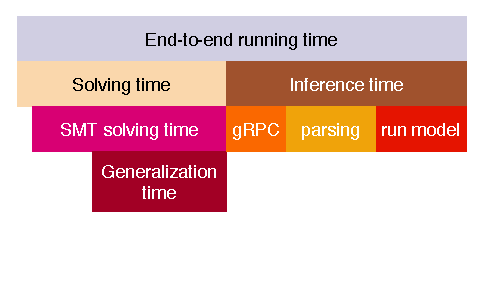
\includegraphics[width=0.6\textwidth]{figures/doping-flame.pdf}
    \caption{\mbox{Runtime~dist.~of~\dpy.}}
    \label{subfig:dpy_vs_spc_ind_gen}
	\end{subfigure}
  \centering
  \begin{subfigure}[b]{0.48\textwidth}
  \centering
    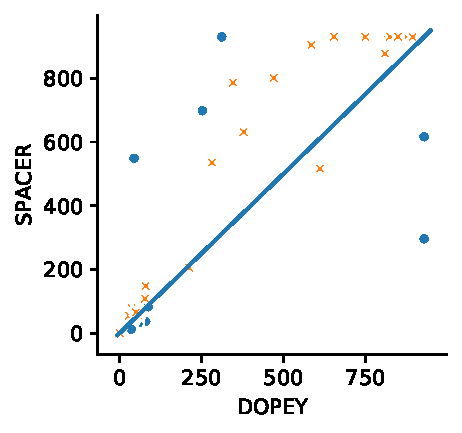
\includegraphics[width=0.99\textwidth]{figures/res-dpy_vs_spc_total.pdf}
    \caption{Solving + infer. time.}
    \label{subfig:dpy_vs_spc_total}
	\end{subfigure}
  \begin{subfigure}[b]{0.48\textwidth}
  \centering
    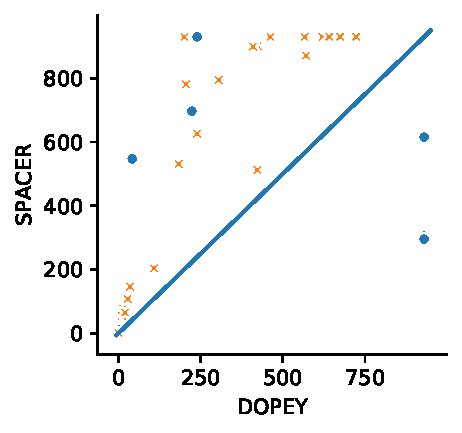
\includegraphics[width=0.99\textwidth]{figures/res-dpy_vs_spc_total_inside.pdf}
    \caption{Solving time.}
    \label{subfig:dpy_vs_spc_total_sub}
  \end{subfigure}
  \begin{subfigure}[b]{0.48\textwidth}
  \centering
    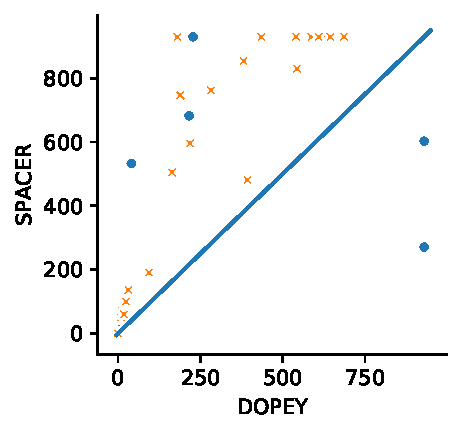
\includegraphics[width=0.99\textwidth]{figures/res-dpy_vs_spc_smt_solver.pdf}
    \caption{SMT-solving time.}
    \label{subfig:dpy_vs_spc_smt}
	\end{subfigure}
  \begin{subfigure}[b]{0.48\textwidth}
  \centering
    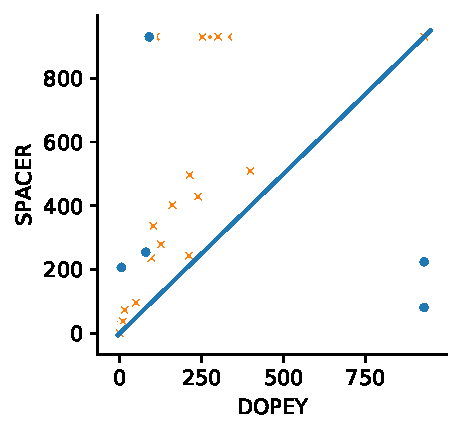
\includegraphics[width=0.99\textwidth]{figures/res-dpy_vs_spc_indgen.pdf}
    \caption{Gen. time.}
    \label{subfig:dpy_vs_spc_ind_gen_sub}
	\end{subfigure}

	\caption{Comparing \dpy's and \spc's running time, where blue dot ({\color{blue}\textbullet}) indicates an instance with unsafe property,  orange cross ({\color{orange}\textbf{x}}) indicates an instance with safe property, top (right) most place are instances \spc (\dpy) timed out.}
% 	\xs{remove the lengend, get rid of square shapes in the plot} }
  \label{fig:dpy_vs_spc}
\end{figure*}



\begin{figure}[t]
  \centering
  \begin{subfigure}{0.48\textwidth}
  \centering
    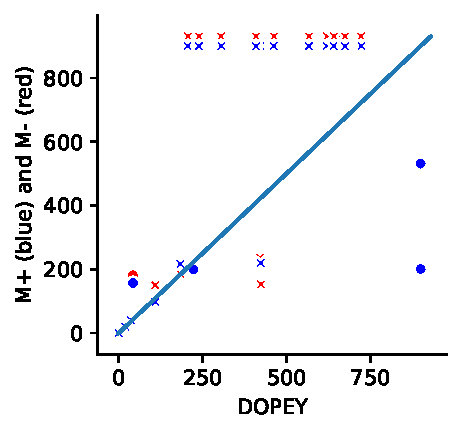
\includegraphics[width=0.99\textwidth]{figures/res-PN_vs_dpy_solving.pdf}
    \caption{Solving time.}
    \label{subfig:flame}
  \end{subfigure}
  \begin{subfigure}{0.48\textwidth}
  \centering
    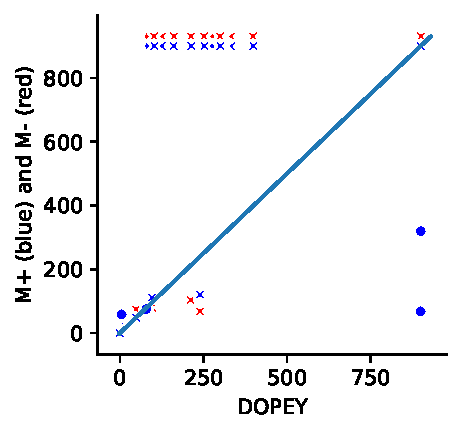
\includegraphics[width=0.99\textwidth]{figures/res-PN_vs_dpy_ind_gen.pdf}
    \caption{Gen. time.}
    \label{subfig:dpy_vs_np_total_sub}
	\end{subfigure}
\caption{\dpy vs. using only either {\color{blue}$\Mpos$} or {\color{red}$\Mneg$}.}
\label{fig:dpy_vs_np}
\end{figure}
\begin{table}[t]
  \centering
  \small
  \renewcommand{\arraystretch}{1.2}
\begin{tabular}{@{}lccc@{}}\toprule
    & All & Unsafe & Safe\\
  \midrule
    Solving + infer. time & 1.51 & 1.50 & 1.58\\
    Solving time & 2.16 & 2.46 & 2.02\\
    SMT solving time & 2.25&2.71&2.08\\
    % Generalization + infer. time & 1.58 & 1.06 &1.67\\
    Generalization time & 3.26& 3.63 & 1.67\\
    \bottomrule
\end{tabular}
\caption{\dpy's speed up compared to \spc on instances solved by both.}
\label{tab:dpy_vs_spc}
\end{table}
%%% Local Variables:
%%% mode: latex
%%% TeX-master: "0.0_main"
%%% End:


\paragraph{Implementation and optimizations.}
\tool is implemented in Python using PyTorch \cite{pytorch}, while \spc is implemented in C++. 
The communication overhead between these two could diminish the performance gain by fast inductive generation, creating an engineering challenge.  
Simply exchanging information via file IO is too expensive.
Instead, we implement a client-server architecture in which \tool is wrapped in a gRPC server connects to a gRPC client inside \spc.
As communicating and parsing over gRPC dominates the overhead, we explore further optimizations. 

% As detailed in Alg \ref{alg:qdrop}, at runtime, \spc sends over a lemma as a string, a list of literals that was kept, and , which will then be parsed in the server side using PySMT into a list of AST, then fed 

First, we use \emph{caching}. Generalizing a lemma triggers multiple requests to \tool. For each request, \dpy sends over a lemma, the server parses it and runs $\Mneg$ and $\Mpos$.
Since multiple requests over a period share the same lemma, we can parse it once and cache the result until a flag indicating \tool needs to handle a new lemma.

Second, we use \emph{parallel precomputation}. Instead of invoking $\Mneg$ and $\Mpos$ once for each literal pair, we \emph{precompute} the full co- and anti-occurrence matrices at once, and use them for \emph{all} subsequent requests.
As long as the matrices fit into the GPU memory, computing the full matrices take the same time as computing one pair of literals.

% To close the performance gap between native \spc and \dpy (\spc + gRPC + \tool), we implement multiple optimizations utilizing as much caching as possible. Recall from the discussion above that \dpy may suggests a wrong lemma candidate, so generalizing one lemma $\ell$ with \dpy may trigger more than one request to \tool. For each request, \spc has to send over a lemma, the server side has to parse it, and we need to run $\Mneg$ and $\Mpos$ to produce the candidate lemma. We want to reduce the number of parsing, and the number of time we need to call the two models.
% First, we notice that the lemma stays the same for the entire run of \tool, so we can parse it once and cache the result. This optimization also reduces the need for sending over the lemma $\ell$: we only need to send it at the beginning of the run, and only a flag indicating whether \tool has finished or not for the later requests.
% More importantly, we can \emph{precompute} the full $\Pneg$ and $\Ppos$ matrices for the lemma $\ell$, cache the results, and use them for \emph{all} the subsequent requests. Due to batching, as long as the matrices fit into the GPU memory (our GPU with 4GBs of memory can easily fit two matrices from any lemma in the benchmark during inferencing), computing the full matrices take the same time as computing one pair of literals!
Together, the two optimizations reduce overhead by up to 50\%. Although gRPC
communication and parsing still dominates the inference time, empirically it is
good enough to achieve absolute speedups. 


%%THINGS TO APE
% Combining predictions
% With our predictions of the criticality a terminalgand oftime saved by removingg, we must make a final decision onwhether or not we should removeg. To do this, we take thetop three terminals with the greatest average positive impacton synthesis time over the training set, as computed withAg. These tended to be terminals that mapped between typeswhich saved more time due to the internal mechanisms andheuristics of the CVC4 solver. We then use the final votingvector from our criticality prediction to choose only two outof the three to remove fromGto formG⋆. We chose to re-move only two terminals fromGin order to minimize thelikelihood of generating aG⋆, such thatπ(G⋆)⊆π(Gcrit).We conjecture that the number of terminals removed is agrammar-dependentparameter that must be selected on a pergrammar basis, just as the number of terminals withAg>0is grammar specific.
% Falling back to the full grammar
% There is some danger thatG⋆will, in fact, not be sufficientto synthesize a
% program. Thus, we propose a strategy that•first, tries to synthesize a program
% with the grammarG⋆•second, if synthesis withG⋆is unsuccessful, falls back
% toattempting synthesis with the full grammarG.We determine how long to wait
% before switching fromG⋆toGby finding anxthat minimizes:

%%% Local Variables:
%%% mode: latex
%%% TeX-master: "0.0_main"
%%% End:

% \NL{spc: smt.total vs }
%  spacer:
%  :time.spacer.solve                                   877.50
%  :time.pool_solver.smt.total                          829.39
% exp: line 5 and line 6 should be more or less the same
% dpy:
%  :time.spacer.solve.reach.gen.bool_ind.outside_spacer 239.81

%  :time.pool_solver.smt.total                          543.69
%  spc :time.spacer.solve                                   810.61

% \begin{figure}[t]
%   \centering
%   \includegraphics[width=0.3\textwidth]{LaTeX/figures/metric-illustration.pdf}
%   \caption{Running time distribution of \dpy.}
%   \label{fig:metric}
% \end{figure}


\section{Empirical Evaluation}
\label{sec:dopey-exp}

\subsection{Setup.} 
We collect benchmarks from \chccomp\cite{CHC-COMP-18} with a particular focus on benchmarks 
%from the Linear Real Arithmetics track  
that corresponds to verification of hybrid systems, which are known to be challenging for inductive generalization, and for which \spc behaves poorly.
We train \dpy on execution traces of 17 benchmarks (or hybrid systems) and test \dpy on other 170 verification tasks (i.e., 10 different properties for each benchmark).
% , which use different safe properties for the same set of hybrid systems.

% For each benchmark, we create 10 variants of it by changing every non-zero constant $v$ in the $\Bad$ property into a uniformly picked value in the range $[0.95 \times v, 1.05 \times v]$. There are 69 such benchmarks, in which \spc was able to solve 37 of them in our time limit of 15 minutes. 
% Among those 37 benchmarks, 20 of them has at least one entry in $\Ppos$ and $\Pneg$ 
% We focus our evaluation on those benchmarks: the intuition is because \dpy is trained using trace generated by \spc, if \spc failed to solve a benchmark, learning a predictor from its trace will not help solving it.
\noindent
\subsubsection{Training details.} 
We train our model using Adam optimizer \cite{adam}, with embedding dimension of 16 and TreeLSTM' hidden size of 64, dropout rate 0.5, negative sampling rate 5, $\mathit{threshold}$ set to 0.8 for both $\Ppos$ and $\Pneg$. Each model is trained up to 3,000 epochs. All experiments are done using an Ubuntu 20.04 PC with an Nvidia 1050 Ti. 

% \noindent 
% \textbf{Evaluation Metrics.}
% We evaluate \dpy and \spc on a) solving time - time spent on solving an instance b) inductive generalization time - time spent on inductive generalization to solve an instance c) SMT-solving time - time spent on solving SMT-queries to solve an instance d)Inferencing time - time \dpy spends on communicating with \spc, parsing the data, and running model inference.
% Note that by randomly mutating the properties, some can become too hard for \spc and \dpy: in total \spc times out on 43 variants, while \dpy times out on 42 variants, 32 of them are timeout by both.

\subsection{Comparing \dpy with \spc.} 
\dpy successfully solved 41 instances on which \spc failed.\footnote{According to
  \chccomp, failure means no result is produced in 15 minutes.} 
On instances solved by both, the speedups achieved by \dpy are summarized in 
\cref{tab:dpy_vs_spc}. The first column lists the running time of different phases of \dpy, of which the distribution is illustrated in \cref{subfig:flame}. The ``All'', ``Unsafe'', ``Safe'' columns show the average speedups for all instances, instances with unsafe properties (i.e. a counterexample is found), instances with safe properties (i.e. a proof is found), respectively. 
The second row shows that \dpy is 1.51$\times$ faster than \spc on average over all instances solved by both.
The last three rows show the average speedups in specific phases.
% \cref{fig:dpy_vs_spc} and \cref{tab:dpy_vs_spc} show the running time comparision of \dpy vs. \spc. Measuring wallclock time, \dpy is 1.5 times faster than \spc on average, and as shown in \cref{subfig:dpy_vs_spc_total}, is extremely effective on large benchmarks, where the overhead can be offset by gains in skip checking useless queries and try to drop multiple literals together.

% Furthermore, if we exclude inferencing time, which potentially could be shorten with more engineering effort, then \dpy is almost always faster, and on average more than twice as fast compare to \spc, as shown in \cref{subfig:dpy_vs_np_total_sub} and \cref{tab:dpy_vs_spc}. This give us an idea about the upperbound of what \dpy can achieve.

% We also observe a big speedup in inductive generalization: on average, \dpy is 1.58 times faster than \spc for inductive generalization, and 3.26 times faster if we exclude the inferencing time.

Beyond quantitative improvements, \dpy also achieved higher quality of inductive generalization, indicated by the safe instances (Safe column in \cref{tab:dpy_vs_spc}). 
Suppose all the performance gain is from the inductive generalization alone, then the speedups should \emph{decrease} when the overall solving time or SMT solving time is considered (as in the Unsafe column of \cref{tab:dpy_vs_spc}). Surprisingly, this is not the case. 
Our analysis shows that this is because \dpy learns \emph{better} lemmas and improves the reasoning steps \emph{outside} of the inductive generalization phase (SMT-solving time)! %This is welcome but unexpected.
%
    
%Beyond quantative improvements, \dpy also achieved higher quality of inductive generalization, which is indicated by instances with safe properties (shown in the ``safe'' column).
%Suppose the performance gain only comes from inductive generalization, the speedups should \textit{decrease} when we gradually zoom out from the generalization phase, however, this is surprisingly not the case. 
%Our analysis shows that this is because \dpy actually learns better lemmas and improves the reasoning steps \textit{outside} of the inductive generalization phase, which is beyond our expectation.

% However, one might expect to see a similar pattern in \cref{subfig:dpy_vs_spc_total_sub} and \cref{subfig:dpy_vs_spc_ind_gen_sub}, as well as \cref{subfig:dpy_vs_spc_total} and \cref{subfig:dpy_vs_spc_ind_gen}: if other components are not affected, we can expect all the performance gain in solving time can only come from gain in inductive generalization. Yet, somewhat surprisingly, we observe that \dpy generalizes not just faster, but also to \emph{better} lemmas! This can be observed by its effect on other SMT-queries in the system: \cref{subfig:dpy_vs_spc_smt} shows that \dpy always spent less time in SMT-solving, which closely correlate with solving time in \cref{subfig:dpy_vs_spc_total_sub}.

\cref{fig:dpy_vs_spc} plots the running time of each individual instance by \dpy and \spc. Except for a few instances whose solving time is short, \dpy significantly outperforms \spc.

\subsection{Ablation study.}
To highlight the combined benefits of $\Mpos$ and $\Mneg$, we also evaluate \dpy with a \textit{single} model. As shown in \cref{fig:dpy_vs_np}, except for a few outliers, using both models is faster and solves more instances -- \dpy times out on 54 (58) instances when using only $\Mpos$ ($\Mneg$).
% We also evaluate the effect of using $\Mpos$ and $\Mneg$ in isolation. As shown in Figure \ref{fig:dpy_vs_np}, while $\Mpos$ and $\Mneg$ by itself could be faster than \dpy, ultimately they also time out more often: $\Mpos$ times out 54 times, while $\Mneg$ times out 58 times. Out intuition is that $\Mpos$ by itself keeps too many redundant literals, making the generalized lemmas not strong enough, thus makes the whole solving diverge. On the other hand, $\Mneg$ by itself doesn't have many chances to contribute: in our benchmarks, $\Mneg$ suggests a candidate at least once in only 48\% of the benchmarks, meaning that most of the time $\Mneg$ by itself is exactly like \textsc{IterDrop}, but with all the overhead of \dpy.
% \NL{Bug in plotting M+ and M-. M- should look very similar to Spc.}


% Sketch:

% \begin{itemize}
%     \item our implementation
%     \item Datasets and baselines
%     \item Evaluation questions
%     \begin{itemize}
%         \item Do we learn a signal? Does the signal transfer? Does learning that signal helps \spc.
%         \item key result: \tool accelerates \spc on solving \textit{similar} instances
%         \item performance analysis with profling stats (which parts get improved, which parts introduce extra overhead)
%         \item transferability?
%         \item ablation study, e.g. different representations, negative/positive/combined models
%         \item highlight some examples
%     \end{itemize}
%     % \item have some fancy diagrams
% \end{itemize}

% \subsection{Implementation details}
% We implement, train, and run our neural network using PyTorch \cite{pytorch} and communicate with the main solver through gRPC. For each lemma, we only send the lemma formula to the oracle once, and parse, precompute and cache $P\_mat$ and $N\_mat$. For every subsequent call to $query\_model$, we only send over $kept\_lits$ and $2b\_checked\_lits$, which are 2 arrays of indices.

% \subsection{Dataset}

% We evaluate \tool on X LRA benchmark queries from CHC-Comp18 \cite{chccomp18}. CHC-Comp is an annual competition where state-of-the-art solvers compete to solve not just hard and practical problems in the industry, but also handcrafted problems those are specifically design to expose the weaknesses of the current solvers. 

% For each query Q in the benchmark, we use \spc to solve it within a time limit of 15 minutes, and record the inductive generalization trace. We then using this trace to train a model specific to Q, and use it as an oracle for 5 randomly mutated variants of Q. We compare solving time of \tool and \spc on the original query and those 5 variants, using 2 metrics: 1) total solving time, and 2) total solving time inside the solver only (time spent on communication, parsing, and inferencing are not counted). While we do not take training time into the comparison, we report here that training one model takes about 2 hours on a 1050Ti.



% We first train \tool using the data generated by solving those queries, and use \tool as an oracle in solving randomly modified variants of the original queries. We then compare the results against \spc\, the state-of-the-art CHC solver. Since \spc\ is written purely in C++, whereas \tool runs the prediction in a Python process, communicate with the main solver through gRPC, we compare them using both the \textbf{total} solving time and \textbf{inside-solver} solving time (any time spent outside the solver, including communication time, parsing time, and inferencing time, is not included).

%%% Local Variables:
%%% mode: latex
%%% TeX-master: "0.0_main"
%%% End:

\section{Conclusion}
\label{sec:2-conclusion}
 We proposed a neuro-symbolic system, \dpy, which uses deep learning models to improve symbolic model checking.
 \dpy uses a positive and a negative model to approximate co- and anti-occurrences of literals appeared in past inductive generalizations.
 The logical and neural component of \dpy are implemented as an efficient gRPC client-server architecture.
 Our empirical evaluation on \chccomp indicates significant improvements of \dpy over the state-of-the-art SMC engine, \spc: inductive generalization is $3.26\times$ faster, and total solving time is $1.51\times$ faster. To the best of our knowledge, \dpy is the first neural-symbolic SMC guidance that works well in practice. We open source the code and welcome contributors to contribute, improve and extend \dpy.

This chapter is adapted from our collaboration with Dr.Xujie Si, and is currently under submission.
\chapter{Reinforcement Learning Guided Software Debloating}
\label{chap:doccam}
\section{Introduction}
\label{sec:intro}

The rapid increase of software productivity in the last decades was fueled by the
extensive use of abstraction and reuse of software components. While this
enabled building larger and more complex software systems, these gains came at
the expense of less efficient and less secure software systems, and contribute
to a troublesome trade-off between productivity and performance/security. When
an application built using general-purpose components is deployed, the majority
of the general-purpose functionality is never used. This creates two problems:
first, as the use of abstraction layers makes it more difficult to optimize the
software, this has a detrimental impact on performance; second, it increases the
attack surface for security vulnerabilities.

% Ashish: While OCCAM, Trimmer, (and Chisel, via tests that the delta-debugged version must pass) specialize the application to its deployment context, other debloaters, such as Piece-wise, do not.
An emerging solution to this problem is a set of tools, called \emph{Software
  Debloaters}, that automatically customize a program to a user-specified
environment. One successful approach for software debloating is based on partial
evaluation (PE)~\cite{pe-book} in which a \emph{partial evaluator} takes a
program and some of its input values and produces a \emph{residual}
(or \emph{specialized}) program in which those inputs are replaced with their
values.
%
% AG: not sure why soundness is important at this point of intro
% A sound partial evaluator must ensure that running the residual program on the
% remaining inputs always produces the same result as running the original
% program on all of its inputs.
%
While PE has been extensively applied to functional and logic programs, it was
less successful on imperative C/\cpp programs (with a noteable exception of
\cmix~\cite{Andersen94} and \tempo~\cite{Consel98}). With the advent of
\llvm~\cite{llvm}, several new partial evaluators of LLVM bitcode have arisen
during the last few years (e.g., \llpe~\cite{llpe}, \occam~\cite{occam}, and
\trimmer~\cite{trimmer}). These tools leverage LLVM optimizations such as
constant propagation, function inlining, and others to either reduce the size of
the residual program (e.g., \occam and \trimmer) or improve performance (e.g.,
\llpe).

The key step of a PE-based debloater is to estimate whether specializing (or
inlining) a function results in a smaller (or more secure) residual program.
%Unfortunately, as with most problems in program analysis, this is very difficult.
Specialization naturally increases the size of the code since it adds extra
functions. However, since some inputs in the new functions have been replaced by
constant values, optimizations such as constant propagation, might become
enabled and result in new optimization opportunities that reduce the code size.
Therefore, the decision whether or not a function should be specialized for a
particular call-site is non-trivial. % where the solution must be found
% in a large search space that represents the effects of other specialized call
% sites and all LLVM optimizations applied after those specializations.
Current PE-based software debloaters use naive heuristics. For example, \occam
implements two heuristics of ``never specialize'' or ``always specialize'',
respectively; \trimmer specializes a function only if it is called once in the
whole program. 

In this paper, we present a new approach based on reinforcement
learning (RL) to automatically infer effective heuristics for
specializing functions for PE-based software debloating. RL is a good
fit for the problem for two reasons. First, code specialization
resembles a Markov Decision Process: each decision moves the code from
one state to another, and specialization depends only on the current
state rather than the history of the transformations.  Second, the
quality of debloating can only be measured after all specialization
actions and corresponding compiler optimizations have been
performed. % Rendering approaches like
% supervised-learning inapplicable.

The main challenge in applying RL is in deciding on a good state
representation.  While it is tempting to use the source code (or LLVM
intermediate representation (IR)) as a state, this is not
computationally tractable. The IR is typically hundreds of MBs in
size. Instead, an adequate set of features that captures meaningful
information about the code while avoiding state aliasing is
required. In particular, these features must capture the \emph{calling context}
in order to distinguish between call-sites.

The main contributions of this paper are threefold: (1) calling
context features that enable RL to find a useful heuristic for
PE-based debloating software; (2) implementation of our method in a
tool called \doccam; and (3) evaluation on the reduction of the
program size and number of possible code-reuse attacks, by comparing
our handcrafted features with features learnt automatically via
embedding LLVM IR into a vector space using \insttovec~\cite{inst2vec}.
%
Our initial evaluation suggests that RL is a viable method for
developing an effective specialization policy for debloating, and learning with
handcrafted features is easier than with \insttovec.


\section{Methods}
\label{sec:methods}
\begin{table}[t]
  \centering
    \renewcommand{\arraystretch}{1.2}

    \begin{tabular}{@{}llll@{}}
      \toprule
      \textbf{Callee}& \textbf{Caller} & \textbf{Module} & \textbf{Call-Site}\\ \midrule
      Basic blocks & Basic blocks & Functions & Arguments \\
      Instructions & Instructions & Instructions & Known arguments\\
      Store instructions & Store instructions & Basic blocks &  \\
      Call instructions & Call instructions & Direct calls &  \\
      Branch instructions & Branch instructions &  &  \\
      Loops & Loops &  &  \\
      Uses & Uses &  &  \\
      Influenced branches & Untouched call-sites &  &  \\
      Influenced instructions &  &  &  \\ \bottomrule 

    \end{tabular}
  \caption{RL features. \emph{Influenced instructions
      (branches)} are the those  whose operands have statically known arguments. \emph{Uses} indicates how many times the
\emph{caller} and the \emph{callee} are invoked.}
  \label{tab:features}
\end{table}

In this section, we formulate the debloating problem as a reinforcement learning
problem, describe the learning procedure, and its hyperparameters.

\paragraph{Action, state, and reward.}
To determine whether a call-site should be specialized or not, we train a policy
using reinforcement learning. This requires defining \emph{action},
\emph{state}, and \emph{reward}.

An action is whether to run a code transformation, called
\emph{specialization}, or not. Consider a call to function $\mathit{calleeF}$
with arguments $A$ at a call-site $c_i$. Let $\mathsf{formals}$ be a map from
call-site arguments to their corresponding formal parameters. Let $B$, $B
\subseteq A$, be the arguments whose values are are statically known. Then,
specialization of the call-site does: 
\begin{enumerate}
\item Create a new function $spec\_calleeF(\mathsf{formals}(A \setminus B))$,
  such that the body of $spec\_calleeF$ is identical to the body of the original
  $calleeF$ except that $\mathsf{formals}(B)$ are replaced with their values.
  
\item Perform constant propagation to push forward the information to the
  rest of callee's body, potentially specializing more call-sites in
  the callee.
  
\item Replace $\mathit{calleeF}(A)$ with $spec\_calleeF(A \setminus B)$ at the
  call-site $c_i$.
\end{enumerate}

Note that after specialization, a software debloater
can trigger other optimization passes such as inlining and dead-code
elimination.

A state is a vector capturing
all the relevant information about the code. We experiment with two
state representations: (a)  a vector of hand crafted features (\textbf{\textbf{HF}}),
and (b) an embedding of LLVM IR via \insttovec (\textbf{\textbf{IV}}).

In \textbf{HF}, the state is a concatenation of four feature vectors,
summarized in Table~\ref{tab:features}. They capture relevant
information about the \emph{callee}, \emph{caller}, \emph{compilation
  unit (module)}, and \emph{call-site}. Most features are
self-explanatory, and hence, we focus only on those which are novel or
more relevant for avoiding state aliasing.
%
% capturing information about \emph{The first one} is the traditional
% approach, in which we come up with a handcrafted set of features
% based on our domain knowledge. The state we choose is a
% concatenation of $4$ feature vectors capturing information about the
% \emph{caller}, the \emph{callee}, the \emph{call-site}, and the
% \emph{compilation unit}. The features are summarized in
% Table~\ref{tab:features}.
%
The \emph{state aliasing} problem occurs when two different states
have the same representation in the RL model. In our context, our
features must distinguish between two call-sites in the same basic
block when invoking the same callee with the same arguments if one is
specialized and the other not.  In~\cite{KulkarniCWS13}, the features
\emph{InLoop} (whether a call-site is in a loop), \emph{InlineDepth}
(the current inlining depth), and \emph{currentGraphSize} (how many
instructions are there in the caller, including one added by
inlining), are used to decide inlining.  However, in our case, these
features are insufficient to prevent state aliasing.  Thus, we also
add \emph{Untouched call-sites} that counts the number of call-sites
yet to be processed. Since the call-sites are processed in a fixed
order, \emph{Untouched call-sites} is sufficient to distinguish any
two call-sites in a function.



% but in our case we
% realized that those features are not enough to prevent state aliasing: 2
% call-sites in the same basic block invoking the same callee with the same
% arguments will have the same value for these features, assuming the first
% call-site is not specialized (i.e there is no change in the caller). We use one
% addition feature to indicate the position of the call-site inside the caller: how
% many call-sites are not visited yet. Because the call-sites are visited in order,
% this feature is enough to distinguish the two call-sites.



% In this approach, the problem is how to avoid state aliasing between 2
% call-sites from the same compilation unit those have the same caller, the same callee, and the same known
% arguments.


% It is not obvious what calling context feature should be used.

% \cite{KulkarniCWS13} uses \emph{InLoop (whether a call-site is in a loop)},
% \emph{InlineDepth (the current inlining depth)}, and \emph{currentGraphSize
%   (capture the changes in the caller)}, but in our case we realized that
% those features are not enough to prevent state aliasing: 2 call-sites in the
% same basic block invoking the same callee with the same arguments will have
% the same value for these features, assuming the first call-site is not
% specialized (i.e there is no change in the caller).  We use one addition feature
% to indicate the position of the call-site  inside the caller: how many call-sites are not visited yet. Because the
% call-sites are visited in order, this feature is enough to distinguish the two
% call-sites. 

In \textbf{IV}, we use \insttovec embedding from~\cite{inst2vec}. We extract the LLVM IR
of the \emph{caller}, the \emph{callee}, and the \emph{calling context} (a window of
$n$ instructions around the call-site) as a lists of instructions. Each
instruction is embedded into a vector space using \insttovec. Additionally, we
encode the arguments at the call-site as a bitvector, in which each statically
known argument  is encoded by $1$, and an unknown argument by $0$. This
bitvector is then embedded using a different embedding matrix.
%During training, the \insttovec
%embedding is fixed while the bitvector embedding matrix is trained. 
% Ashish: Can we say more about the "bitvector is then embedded using a
% different embedding matrix"? Can the matrix be explained intuitively?
% Nham: addressed.
Finally, the \textbf{IV} state is a tuple of the above four $2$-D matrices. 
% Ashish: Is "2-D" redundant above?
Note that in this case,
the calling context of each call is explicitly represented by the IR.


%The calling context is explicit with this approach.


  


%% from GSA paper

%%%%%%%%%%%%%%%%%%%%%%%%%%%%%%%%%%%%%%%%%%%%%%%%%%%%%%%%%%%%%%%%%%%%%%%%%%%%%%%%%%%%%%%%%%%%%%%%%%%%%%%%%%%%%%%%%%%%%%%%%%%%%%%%%%%%%%%%%%%%%%%%%%%%%%%%%%%%%%%%%%%%%%%%%%%%%%%%%%%%%%%%%%%%%%%%%%%%%%%%%%%%%%%%%%%%%%%%%%%%%%%%%%%%%%%%%%%%%%%%%%%%%%%%%%%%%%%%%%%%%%%%%%%%%%%%%%%%%%%%%%%%%%%%%%%%%%%%%%%%%%%%%%%%%%%%%%%%%%%%%%%%%%%%%%%%%%%%%%%%%%%%%%%%%%%%%%%%%%%%%%%%%%%%%%%%%%%%%%%%%%%%%%%%%%%%%%%%%%%%%%%%%%%%%%%%%%%%%%%%%%%%%%%%%%%%%%%%%%%%%%%%%%%%%%%%%%%%%%%%%%%%%%%%%%%%%%%%%%%%%%%%%%%%%%%%%%%%%%%%%%%%%%%%%%%%%%%%%%%%%%%%%%%%%%%%%%%%%%%%%%%%%%%%%%%%%%%%%%%%%%%%%
% Code Reuse Attacks: Code reuse attacks are a class of attacks in which an attacker compromises the control flow of a pro-gram and redirects execution to an existing executable part of the  program  to cause  a  malicious  effect,  bypassing  code in-jection  defensessuch  as  Write  XOR  Execute.In  gadget-based code reuse attack methods such as ROP, JOP, and COP [7, 21, 8, 9], the attacker chains together short instruction se-quences  called  gadgets present  in  the  program  in  a  specific order to construct a malicious payload without injecting code. %
%%%%%%%%%%%%%%%%%%%%%%%%%%%%%%%%%%%%%%%%%%%%%%%%%%%%%%%%%%%%%%%%%%%%%%%%%%%%%%%%%%%%%%%%%%%%%%%%%%%%%%%%%%%%%%%%%%%%%%%%%%%%%%%%%%%%%%%%%%%%%%%%%%%%%%%%%%%%%%%%%%%%%%%%%%%%%%%%%%%%%%%%%%%%%%%%%%%%%%%%%%%%%%%%%%%%%%%%%%%%%%%%%%%%%%%%%%%%%%%%%%%%%%%%%%%%%%%%%%%%%%%%%%%%%%%%%%%%%%%%%%%%%%%%%%%%%%%%%%%%%%%%%%%%%%%%%%%%%%%%%%%%%%%%%%%%%%%%%%%%%%%%%%%%%%%%%%%%%%%%%%%%%%%%%%%%%%%%%%%%%%%%%%%%%%%%%%%%%%%%%%%%%%%%%%%%%%%%%%%%%%%%%%%%%%%%%%%%%%%%%%%%%%%%%%%%%%%%%%%%%%%%%%%%%%%%%%%%%%%%%%%%%%%%%%%%%%%%%%%%%%%%%%%%%%%%%%%%%%%%%%%%%%%%%%%%%%%%%%%%%%%%%%%%%%%%%%%%%%%%%%%%%
For rewards, we focus on two different metrics. First, we measure the
number of instructions in the final binary produced by the software debloater
after specialization took place. Second, we measure the reduction of the
\emph{attack surface}, focusing on code reuse attacks.

\emph{Code reuse attacks} are exploits in which an attacker makes use of the
available instructions in the binary to chain together short sequences called
\textit{gadgets}, and use those gadgets to compromise the control flow of the
program, causing a malicious effect. Those sequences are often categorized based
on their last instruction, into ROP (return-oriented programming), JOP
(jump-oriented programming), and COP (call-oriented programming) gadgets,
respectively. Since the relationship between the number of gadgets and
exploitability is an open question~\cite{gsa}, we focus on reducing the number
of gadgets without making any further claim about the security of the debloated~code.

The rewards are the negations of the number of instructions, ROP, JOP, and COP
gadgets. The negation is necessary because we are interested in minimizing our
metrics. We only have one measurement at the end of an episode (when the final
binary is produced). Immediate rewards after each action are set to zero.
\paragraph{Learning procedure, policy network, and hyper-parameters.}
Each state representation requires a different neural net for the policy network.
%
For \textbf{HF}, we use a $3$-layer fully connected network. Before training, we run the
pipeline with a random policy $100$ times to calculate the mean and standard
deviation of each feature, and use this metadata to normalize all features into
mean of $0$ deviation of $1$.

For \textbf{IV}, we run the \emph{caller}, the \emph{callee}, the \emph{calling context}
and the \emph{arguments bitvector} through four separate $2$-layer
GRU~\cite{gru} blocks, concatenate the last hidden outputs of these $4$ blocks,
and then feed it to a $3$-layer fully connected network. The architecture is
depicted in Fig.~\ref{fig:inst2vec_occam}.

Both networks use ReLU~\cite{relu} as the activation function. 
% Ashish: Should a citation be added for ReLU above?
We use \reinforce~\cite{reinforce} with normalized rewards to update
the policy for both models. At each \reinforce iteration, we roll out
$k$~runs of the current policy, batch them together, and use the Adam
optimizer~\cite{adam} to update the network. For all metrics, we use the same
hyper-parameters: \insttovec calling
context $n = 10$, number of runs in each policy rollout $k =75$, Adam's learning rate = $0.001$, and train up to $340$ iterations.

     \begin{figure}
         \centering
         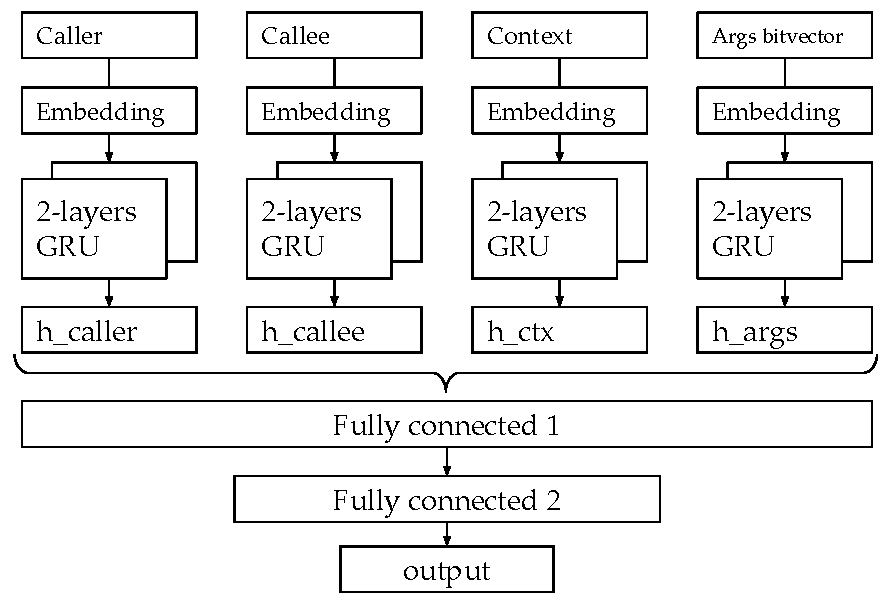
\includegraphics[width=0.75\textwidth]{doccam_figures/inst2vec_occam.pdf}
         \caption{Policy network architecture using \insttovec .}
         \label{fig:inst2vec_occam}
     \end{figure}
     \begin{figure}
         \centering
         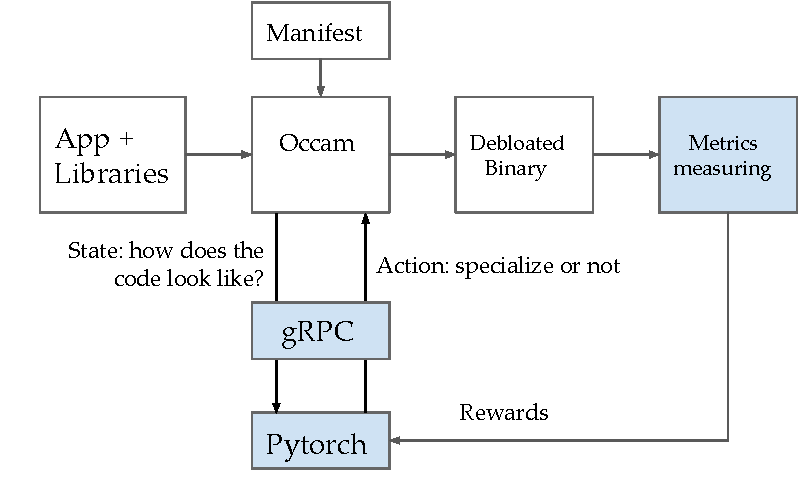
\includegraphics[width=0.75\textwidth]{doccam_figures/D-OCCAM.pdf}
         \caption{\doccam architecture. Boxes in blue correspond to this work.}
         \label{fig:d-occam}
     \end{figure}


%%% Local Variables:
%%% mode: latex
%%% TeX-master: "neurips_2019"
%%% End:

%%% Local Variables:
%%% mode: latex
%%% TeX-master: "neurips_2019"
%%% End:

\section{Implementation and Evaluation}

We have implemented our prototype, called \doccam,
using \occam~\cite{occam}. The architecture of \doccam is depicted in
\cref{fig:d-occam}.
%
\doccam takes as inputs a set of LLVM modules (main application and
libraries) and a manifest (i.e., a user-defined execution environment)
and produces a specialized binary.
%
We used Gadget Set Analyzer (\gsa)~\cite{gsa} to evaluate 
 the specialized binary and
\pytorch~\cite{pytorch} for training the deep learning~models. % The communication between \occam and \pytorch is via gRPC
 
% channels.
At each call-site, \occam calculates the features
described in \cref{tab:features} from the \llvm module, sending them to the \pytorch server, and
transforming the code based on the returned decision.
%
During inference, the \pytorch server receives the message and runs the learnt
policy to decide whether to specialize that
call-site. During training, the \pytorch server also keeps track of all the
decisions it has made and uses that information to update its
policy. We run multiple copies of \occam on multiple copies of the \pytorch
server to scale up the learning process, which is justified by the Markov property of the state.%  sumed, we can easily
% run multiple copies of \occam on multiple codebases at the same time with just a
% single \pytorch server: to pick the action for a call-site, the server
% needs exactly one message from \occam. Hence, we do not have to keep
% track of where the messages are coming from and their history.


%% \subsection{Implementation details}
%% In order to implement our pipeline, we need two building blocks: one for
%% analyzing and interacting with the source code, and one for training
%% and using deep learning models. We choose to use LLVM \cite{llvm} for the former part,
%% and PyTorch \cite{pytorch} for the latter. Furthermore, we need a communication layer between
%% them. We chose gRPC for its simplicity and performance. 

%% We build our framework on top of \emph{OCCAM} \cite{occam}. The architecture is depicted in Figure
%% ~\ref{fig:d-occam}.

%% gRPC channels are added to \occam to communicate with the PyTorch server. At each call-site, \occam is
%% responsible for profiling the module to extract the 4 vectors mentioned in
%% Section~\ref{subsec:asr}, sending them to the PyTorch server, and transforming the code
%% based on the returned decision.

%% During inference, the PyTorch server receives the
%% message, runs the learnt policy to decide whether or not \occam should specialize
%% that call-site. During training, the PyTorch server also keeps track of all the
%% decisions it has made, and use that information to update its policy. With the
%% Markov property of the state assumed, we can easily run multiple \occam on multiple
%% codebases at the same time with just a single PyTorch server: to pick the
%% action for a call-site, the server needs exactly one message from \occam. Hence,
%% we do not have to keep track of where the messages are coming from and their history.

%%%%%%%%%%%%%%%%%%%%%%%%%%%%%%%%%%%%%%%%%%%%%%%%%%%%%%%%%%%%%%%%%%%%%%%%%%%%%%%%%%%%%%%%%%%%%%%%%%%%%%%
% The architecture allows great scalability and helps us utilize the right                            %
% hardware for the right job: the Core should be run on machines with strong CPUs,                    %
% while the PyTorch server should be run on machines with strong GPUs. The server could be            %
% written in any deep learning framework to make use of open source                                   %
% implementations of state-of-the-art learning algorithms. While both PyTorch and TensorFlow have C++ %
% bindings, they are not as well supported and documented as their Python counterparts.               %
%%%%%%%%%%%%%%%%%%%%%%%%%%%%%%%%%%%%%%%%%%%%%%%%%%%%%%%%%%%%%%%%%%%%%%%%%%%%%%%%%%%%%%%%%%%%%%%%%%%%%%%

\begin{figure}
     \centering
     \begin{subfigure}[b]{0.4\textwidth}
         \centering
         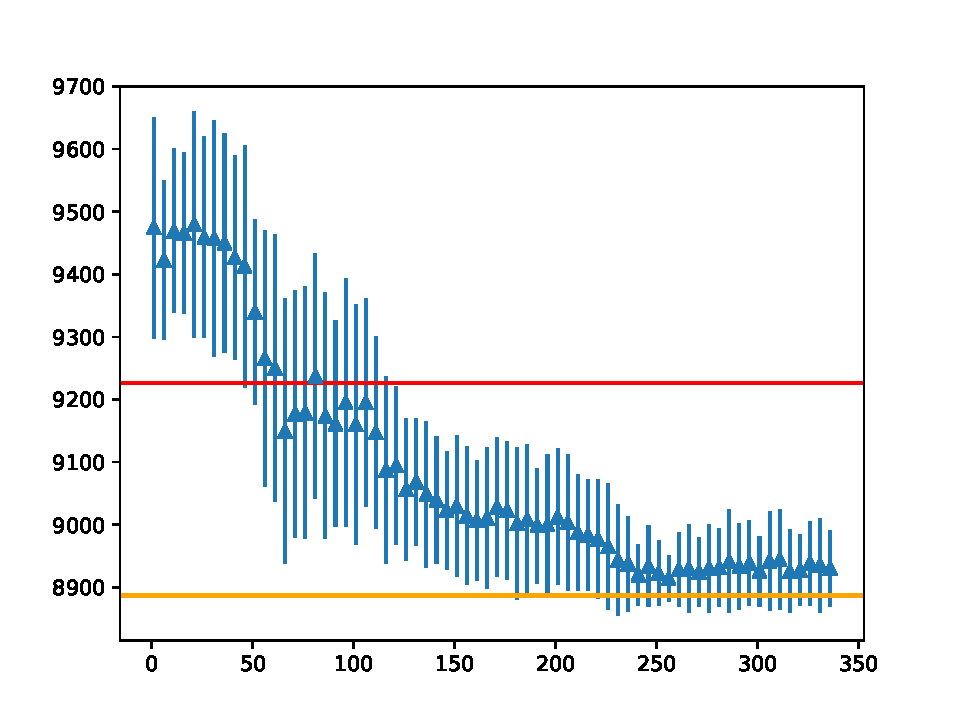
\includegraphics[width=\textwidth]{doccam_figures/tree_hf_lr_0001/Number_of_instructions_75_339_sparsed.pdf}
         \label{fig:inst}
         \vspace{-0.2in}
         \caption{Instructions (\textbf{HF})}
       \end{subfigure}
     \begin{subfigure}[b]{0.4\textwidth}
         \centering
         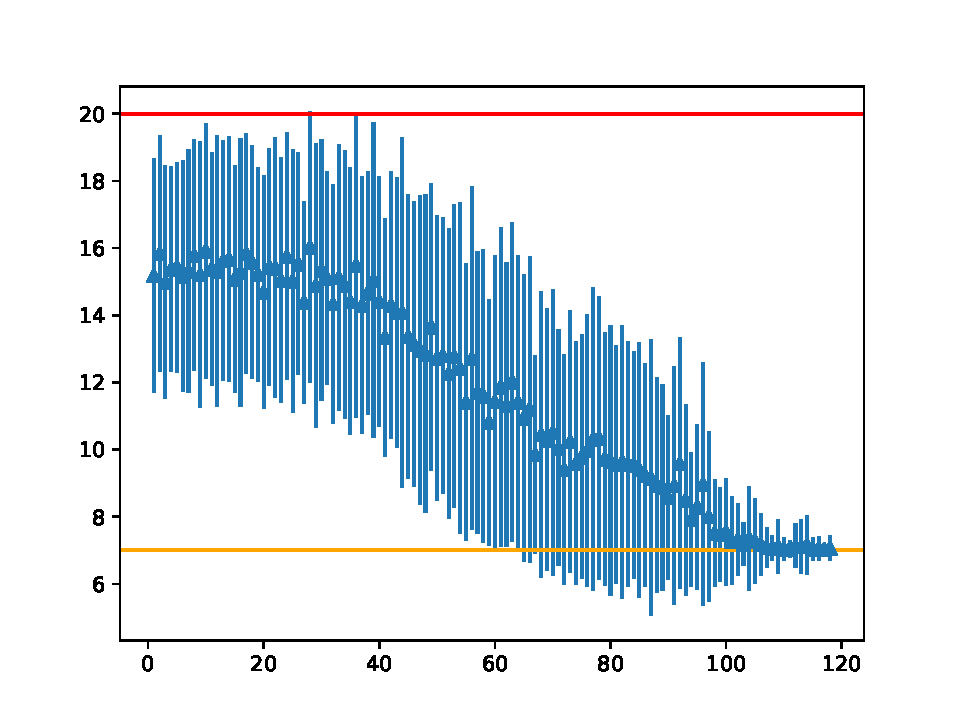
\includegraphics[width=\textwidth]{doccam_figures/tree_hf_lr_0001/COP_gadgets_75_119.pdf}
         \label{fig:cop}
         \vspace{-0.2in}
         \caption{COP gadgets (\textbf{HF})}
       \end{subfigure}
       \begin{subfigure}[b]{0.4\textwidth}
         \centering
         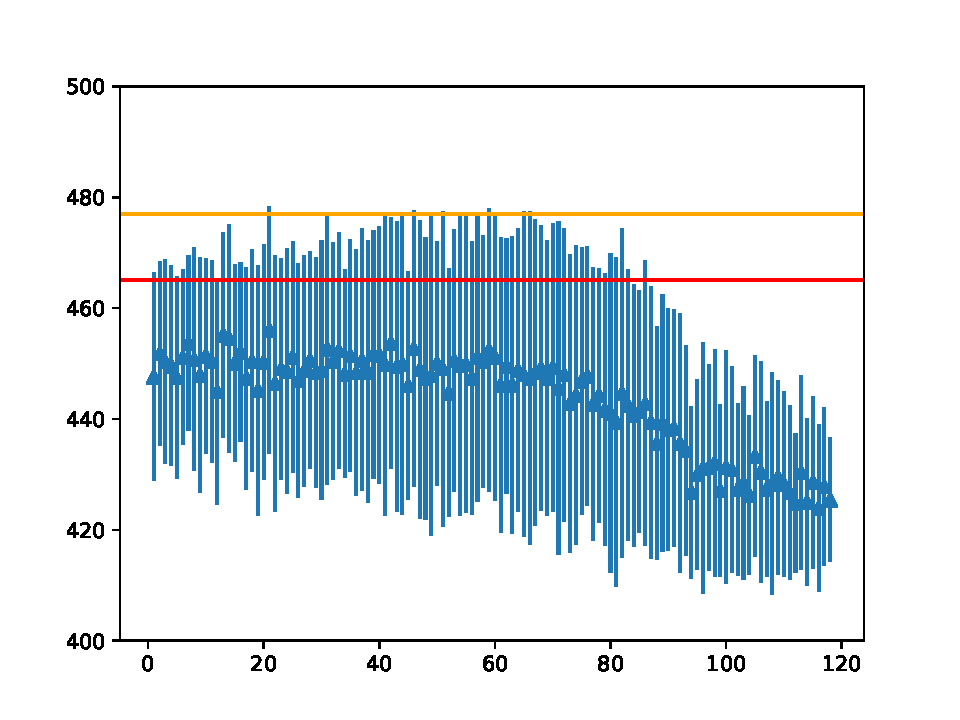
\includegraphics[width=\textwidth]{doccam_figures/tree_hf_lr_0001/ROP_gadgets_75_119_sparsed.pdf}
         \label{fig:rop}
         \vspace{-0.2in}
         \caption{ROP gadgets (\textbf{HF})}
     \end{subfigure}
     \begin{subfigure}[b]{0.4\textwidth}
         \centering
         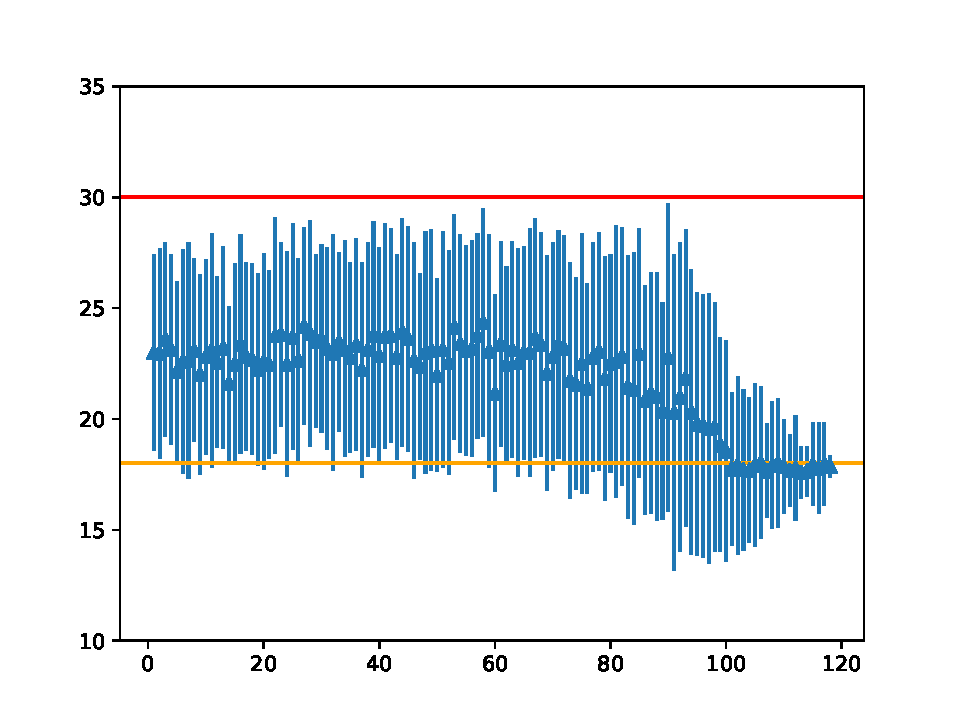
\includegraphics[width=\textwidth]{doccam_figures/tree_hf_lr_0001/JOP_gadgets_75_119_sparsed.pdf}
         \label{fig:jop}
         \vspace{-0.2in}
         \caption{JOP gadgets (\textbf{HF})}
     \end{subfigure}
     \begin{subfigure}[b]{0.4\textwidth}
         \centering
         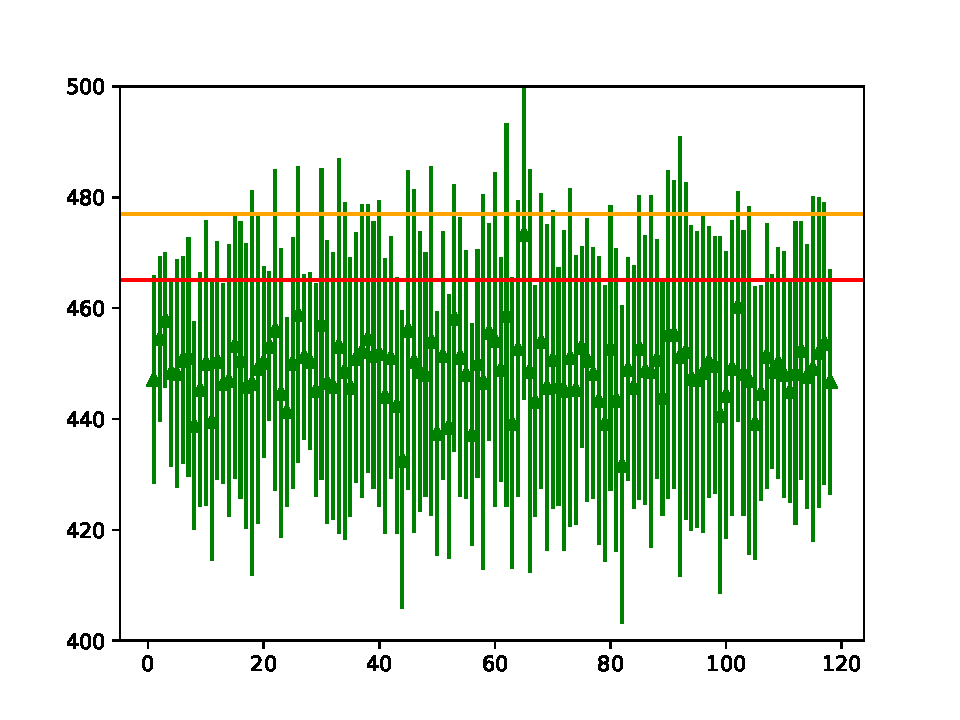
\includegraphics[width=\textwidth]{doccam_figures/tree_iv_lr_0001/ROP_gadgets_20_119_sparsed.pdf}
         \label{fig:inst2vec_rop}
         \vspace{-0.2in}
         \caption{ROP gadgets (\textbf{IV})}
       \end{subfigure}
  \begin{subfigure}[b]{0.4\textwidth}
         \centering
         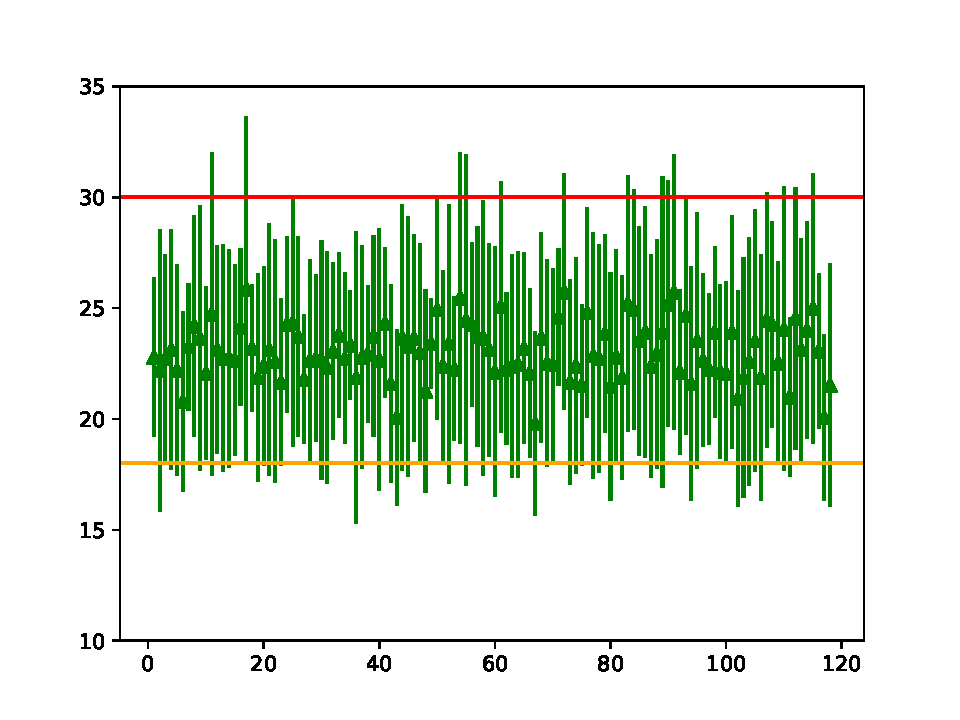
\includegraphics[width=\textwidth]{doccam_figures/tree_iv_lr_0001/JOP_gadgets_15_119_sparsed.pdf}
         \label{fig:inst2vec_inst}
         \vspace{-0.2in}
         \caption{JOP gadgets (\textbf{IV})}
       \end{subfigure}
       \caption{
Results for optimizing different metrics using \textbf{HF} and \textbf{IV}. x-axis is the number
of RL iterations. y-axis is the results. Dots and bars are mean and std. dev. of
$k$ runs in each iteration. \textbf{HF} results are in blue while
\textbf{IV} results are in green. Orange and red lines are \occamo and \occama results, respectively.}
     \label{fig:results}
     \end{figure}



We compare \doccam with \occam running in two modes.
%
First, \occama that runs \occam with a
\emph{nonrecursive-aggressive} policy. This always specializes a
call-site if the callee is not a recursive function.
%
Second, \occamo that runs \occam without specializing any call-site.
%
Fig.~\ref{fig:results} shows the comparision between \doccam using \textbf{HF}
, \doccam using \textbf{IV}, \occama , and \occamo for debloating \gnutree. 
% \nl{discuss the graphs}
On average, \doccam outperforms both \occamo and \occama in reducing the number of
ROP and JOP gadgets, matches \occamo on COP gadgets, and underperforms 
in reducing the number of instructions. Interestingly, while \doccam matches
\occamo on COP, it finds a different policy that specialize some call-sites.
For optimizing the number of instructions, we run 200 more training iterations
but are not able to outperform \occamo. We include the results for the number of
instructions only to demonstrate the flexibility of our approach.
% vNote that optimizing the number of instructions is not our main target, since \doccam relies
% n \llvm to perform other code transformation passes, and \llvm also
% has its own heuristics controlling those passes to reduce the size of the final
% binary. The results for optimizing the number of instructions are included just to
% demonstrate the flexibility of our approach

% \nl{why inst2vec is not working}
In all of our experiments, the learning procedure does not converge when we use
\insttovec pre-trained embedding. Upon closer inspection, we observe that
the software in our test suite, once compiled to LLVM IR, contained many
instructions regarded as low-frequency by \insttovec. Consequently, they are all
mapped into the same \texttt{UNK!} token in the cutoff dictionary. Hence, the
calling context window that we use suffers from the state aliasing problem: different
calling contexts are mapped to the same vector of tokens. 

This is surprising since \insttovec claims to train the embedding on a wide
range of software written in C, C++, FORTRAN, and OpenCL, specifically to avoid overfitting
to a small family of code bases.

%%% Local Variables:
%%% mode: latex
%%% TeX-master: "neurips_2019"
%%% End:

\section{Related work and Conclusions}\label{sec:future}
%\subsection{Related work}
%\paragraph{Compiler optimization using Machine learning}

% \paragraph{Related work}
Recent advances in deep learning and RL have opened new frontiers to the design
of compiler heuristics~\cite{autotuning}. Most current approaches define actions
at the compilation unit level: whether to run a particular optimization pass, or
how to schedule optimization passes. For example, Cummins et al.~\cite{deeptune}
model code as a natural language problem to predict whether to run the code on
CPU or GPU, as well as the optimal GPU thread coarsening factors. Kulkarni et
al.~\cite{KulkarniCWS13} use NEAT --- a genetic algorithm --- to learn an
inlining heuristic for MaxineVM as a neural network. For interpretability, they
then approximate the neural network by a decision tree. We, on the other hand,
use actions at much lower granularity, focusing on specialization at each
call-site.
% Moreover, they do not model the compilation process as a Markov Decision
% Process.

Program code is a rich structure that can be presented in a variety of ways,
e.g., as raw text, control-flow and call- graphs, etc. Recent application of
deep learning for code experiment with models based on techniques from Natural
Language Processing and Graph Neural Network (e.g.,~\cite{code2vec, inst2vec,
  code2seq, code2blah}). Among them, \insttovec~\cite{inst2vec} is the only one
that works on LLVM IR. %Applying \insttovec to \occam was therefore a natural
%choice for us.

The closest related work is Chisel~\cite{chisel} -- a software debloater based
on RL. Inspired by C-Reduce~\cite{creduce}, Chisel takes a program $P$ and a
property of interest $\varphi$ (i.e., $P$ must compile and pass tests defining
$\varphi$) and produces the smallest program $P'$ that satisfies $\varphi$. RL
accelerates the search for the reduced program providing a scalability boost.
Compared to \doccam, Chisel has very different state and action space, and, is generally
only as sound as the test cases defining $\varphi$.

%% Only few are done at deeper levels, such as call-sites.
%% \cite{KulkarniCWS13} is closest to our work, in which the authors use
%% NEAT - a genetic algorithm - to learn an inlining heuristic for
%% MaxineVM in the form of a neural network, then construct a decision
%% tree to approximate the neural network for interpretability. However,
%% \cite{KulkarniCWS13} does not model the compilation process as a
%% Markov Decision Process. \cite{chisel} also uses Reinforcement
%% learning to debloat software, but works on a different action, which
%% is delta debugging. Delta debugging relies on test suites and is not
%% sound, while \emph{specialization} relies on specified execution
%% environments and is sound.

%% \paragraph{PE-based software debloaters:}
%% \trimmer~\cite{trimmer} and \occam~\cite{occam} are two prominent PE-based
%% software debloaters. \doccam is built on top of \occam, which allows the specialization policy to be defined. In contrast, 
%% \trimmer limits call-site specialization to cases where the original functions can be eliminated.

%\paragraph{Deep learning for code:}\label{par:deepcode}

%% Source code is a rich structure that could be viewed as raw texts or
%% graphs. Hence, recent work in deep learning for code has tried to
%% build models based on results in Natural Language Processing and Graph
%% Neural Network \cite{code2vec, inst2vec, code2seq, code2blah}.  Among
%% them, to the best of our knowledge, \insttovec\cite{inst2vec} is the
%% only one that looks at code at the LLVM IR level. Applying \insttovec
%% to \occam was therefore a natural choice for us.

%\subsection{Discussion}
% \paragraph{Conclusions}
In this thesis, we present \doccam --- an end-to-end tool to learn
specialization heuristics for software debloating. Our preliminary results
suggest that it is feasible to use RL to learn an effective specialization
heuristic to optimize a variety of related metrics. They also suggest that out
of the box, pretrained embedding such as \insttovec might not be applicable for the task.
%
% Ashish: Either we should say why "using a deep representation of IR is the way to move forward", or weaken the statement to one such as:
% While our initial foray into embedding the IR into a deep representation (using \insttovec) did not outperform hand crafted features, we believe there is scope to improve this in the future.
%
We hope that \doccam contributions in feature engineering and architecture
might be applicable to other compiler optimization tasks such as inlining.

This chapter is adapted from the following published work:
\begin{itemize}
    \item Nham Le, Ashish Gehani, Arie Gurfinkel, Susmit Jha, Jorge A.Navas, \textit{Reinforcement Learning Guided Software Debloating}, Workshop on ML for Systems at NeurIPS 2019
\end{itemize}
% For future directions, we have 3 directions:                                     %
% \paragraph{Better representation of the code} While the features that we are     %
% collecting is enough for the pipeline to work and shows a positive learning      %
% signal, it is clear that we are only using surface level information about       %
% the code. It is not impossible to have 2 call-sites that have the                 %
% same features that we are using, but have different instructions or order of     %
% instructions in both the caller and the callee, causing state aliasing.          %
% Using embeddings mentioned in ~\ref{par:deepcode} should give us more            %
% information, hence reduce state aliasing and help the learning process.          %
% \paragraph{Better contextual information} There are multiple way we can use to   %
% encode the calling context: a window of \emph{n} instructions before and         %
% after before the call-site, or an attention map at each call-site, etc. Those      %
% encoding will likely provide more information than the feature we are using.     %
% \paragraph{Transfer learning} The pipeline that we are using is online-learning: %
% For each software, we need to relearn everything. There are no learnings         %
% that can be transfered. For small software, we can afford to train REINFORCE     %
% multiple iteration, but the usefulness of this approach is limited when          %
% dealing with large and complex softwares. To learn a general policy that can     %
% work on more than 1 softwares is still an open research problem.                 %
% %                                                                                %
%%%%%%%%%%%%%%%%%%%%%%%%%%%%%%%%%%%%%%%%%%%%%%%%%%%%%%%%%%%%%%%%%%%%%%%%% 
% \item Compare with other software debloaters:                          %
%   \begin{itemize}                                                      %
%     \item The closest related work is \chisel~\cite{chisel} because    %
%       they also use reinforcement learning.                            %
%     \item Apart from \chisel, I'm only aware of                        %
%       Piece-Wise~\cite{piecewise} but it's quite different because it  %
%       only focus on removing dead functions. So we don't probably need %
%       to mention it. Ashish should help here.                          %
%   \end{itemize}                                                        %
%                                                                        %
% \item Compare with compiler optimizations using machine learning       %
%   (e.g., \cite{autotuning,KulkarniCWS13})                              %
%                                                                        %
% \item Compare with recent POPL'19 \codetovec~\cite{code2vec}           %
%                                                                        %
% \end{itemize}                                                          %
%%%%%%%%%%%%%%%%%%%%%%%%%%%%%%%%%%%%%%%%%%%%%%%%%%%%%%%%%%%%%%%%%%%%%%%%%%




%%% Local Variables:
%%% mode: latex
%%% TeX-master: "neurips_2019"
%%% End:

\chapter{Future Work}
\label{chap:future}
Recent advances in deep learning, especially language modeling, has played a tremendous role in solving many natural language reasoning tasks that used to be considered infeasible. Yet, neural-guidance for symbolic reasoning is still a barely charted territory, with successes few and far between.
In previous chapters, we have studied two exciting applications of learning a better heuristic for symbolic reasoning tasks, specifically Inductive Generalization, and Software Debloating.
In this chapter, we outline some future directions on guiding symbolic reasoning using machine learning, which we think are feasible, and will play a major role in making neural-guidance not just another tool, but a powerful hammer in tackling down symbolic reasoning tasks.

\paragraph{Representation learning for formal languages.} Deep learning has made tremendous progress in understanding natural language, and in many cases surpassing human-level \cite{whosaidwhat, whosaidwhat2}. However, there is a big gap between natural language understanding and formal language understanding. Natural language, as a means of transferring information through noisy channels (i.e sound wave through the air, or word-of-mouth gossiping), has a lot of redundancy in both grammar and context \cite{ling_redundancy}. This redundancy helps with, among others, enhancing the comprehensibility of natural language. In contrast, formal languages, such as formulas or programming languages, are designed to be as concise and compact as possible, with little to no redundancy. This makes representation learning for formal languages very challenging. For example, many breakthroughs in NLP are based on the word-guessing tasks --- given a sentence, we randomly remove some words in it, and try to guess them using the remaining words --- such as word2vec \cite{word2vec} or BERT \cite{bert}. Due to redundancy, it is reasonable to try guessing a word from its context, but it is counter-intuitive to try to do the same for formal languages. 

One promising way to learn a good representation for formal languages is to use the structure of the entities. In \cref{chap:dopey}, we show that augmenting an AST with domain knowledge about the tokens can achieve good results on representing linear arithmetic formulas. Given that graph-based and tree-based methods have been successful in structure learning tasks, such as drug discovery \cite{drug_dis}, it is reasonable to believe that representation learning for small to medium mathematical formulas is feasible. While in \cref{chap:doccam}, we cannot transfer results of inst2vec \cite{inst2vec} into our domain, this graph-based work shows promising results in many different tasks, and it is foreseeable that better feature engineering at the token level may help us achieve even better code representation.

\paragraph{Transfer learning for formal languages.} 
One of the main reasons for the wide adoption of deep learning is the success of \emph{transfer learning}. Starting from a model pretrained on millions of labeled images using hundreds of GPU hours, an individual researcher can easily fine tune it for a task that may have only a handful of training examples, using a small amount of computing power. ELMo \cite{elmo} and BERT \cite{bert} were big breakthroughs in NLP for the same reason: previously, each NLP task required a full end-to-end training, making it very difficult to use deep learning to solve NLP problems with small datasets. 

The main challenge in successful transfer learning for symbolic reasoning lies in the fact that downstream tasks are often \emph{representation specific}: while one can imagine a model trained on a dataset about the Python programming language can be helpful to do Python reasoning tasks (e.g neural-based auto-completion), there is little reason to believe it would help detect memory leaks in C++, a bug that is completely missing in Python. This is very different in natural language, where tasks for different languages are often the same: answering questions, analysing sentiments, extracting entities, among others. Because of this reason, while the amount of available code and formulas are tremendous, it is still not clear how one can train a useful general model that can be finetuned to solve multiple different tasks. 

% Nevertheless, in \cref{chap:dopey}, we have explored the possibility of transfer learning between similar problems, and recent works like \cite{lample2019deep} and \cite{neuralsat} shows that it is also feasible to learn heuristics that transfers between a more diverse set of problems in the same task. 
A useful idea that borrowed from the compilers community: at the end of the day, all programming languages have to be compiled to machine instructions. A model trained on this lowest level of abstraction, or some other forms of Intermediate Representation (IR), could be the key to the puzzle. While there is still no pre-trained model that is helpful for multiple tasks in practice, we envision that this is a solvable missing piece to make neural-guidance learning truly useful.

\chapter{Conclusion}
\label{chap:conclusion}
This thesis presents a glimpse into the feasibility of learning state-of-the-art heuristics for symbolic reasoning tasks, specifically, inductive generalization and software debloating, using neural networks.

For inductive generalization, we proposed a neuro-symbolic system, \dpy, which uses a positive and a negative model to approximate co- and anti-occurrences of literals that appeared in past inductive generalizations to improve the overall symbolic model checking process.
For software debloating, we present \doccam --- an end-to-end tool to learn
specialization heuristics using Reinforcement Learning.

In both cases, our results show that the learned heuristics are better than state-of-the-art handcrafted ones, even when we take into account the communication costs between our neural components in Python and our symbolic engine in C++, in the case of \dpy. To the best of our knowledge, they are both the first neural-symbolic guidance that works well in practice for their tasks.

Looking forward, we want to extend the work presented in this thesis to make it more useful, by trying to learn a better representation for the formulas and LLVM IRs, as well as trying to make the learned heuristics transferable to different problems in the same task. 

%----------------------------------------------------------------------
% END MATERIAL
% Bibliography, Appendices, Index, etc.
%----------------------------------------------------------------------

% Bibliography

% The following statement selects the style to use for references.  It controls the sort order of the entries in the bibliography and also the formatting for the in-text labels.
\bibliographystyle{plain}
% This specifies the location of the file containing the bibliographic information.  
% It assumes you're using BibTeX to manage your references (if not, why not?).
\cleardoublepage % This is needed if the book class is used, to place the anchor in the correct page,
                 % because the bibliography will start on its own page.
                 % Use \clearpage instead if the document class uses the "oneside" argument
\phantomsection  % With hyperref package, enables hyperlinking from the table of contents to bibliography             
% The following statement causes the title "References" to be used for the bibliography section:
\renewcommand*{\bibname}{References}

% Add the References to the Table of Contents
\addcontentsline{toc}{chapter}{\textbf{References}}

\bibliography{uw-ethesis}
% Tip 5: You can create multiple .bib files to organize your references. 
% Just list them all in the \bibliogaphy command, separated by commas (no spaces).

% The following statement causes the specified references to be added to the bibliography% even if they were not 
% cited in the text. The asterisk is a wildcard that causes all entries in the bibliographic database to be included (optional).
\nocite{*}
%----------------------------------------------------------------------

% Appendices

% The \appendix statement indicates the beginning of the appendices.
% \appendix
% % Add a title page before the appendices and a line in the Table of Contents
% \chapter*{APPENDICES}
% \addcontentsline{toc}{chapter}{APPENDICES}
% % Appendices are just more chapters, with different labeling.
% \chapter[PDF Plots From Matlab]{Matlab Code for Making a PDF Plot}
\label{AppendixA}
% Tip 4: Example of how to get a shorter chapter title for the Table of Contents 
%======================================================================
\section{Using the Graphical User Interface}
Properties of Matab plots can be adjusted from the plot window via a graphical interface. Under the Desktop menu in the Figure window, select the Property Editor. You may also want to check the Plot Browser and Figure Palette for more tools. To adjust properties of the axes, look under the Edit menu and select Axes Properties.

To set the figure size and to save as PDF or other file formats, click the Export Setup button in the figure Property Editor.

\section{From the Command Line} 
All figure properties can also be manipulated from the command line. Here's an example: 
\begin{verbatim}
x=[0:0.1:pi];
hold on % Plot multiple traces on one figure
plot(x,sin(x))
plot(x,cos(x),'--r')
plot(x,tan(x),'.-g')
title('Some Trig Functions Over 0 to \pi') % Note LaTeX markup!
legend('{\it sin}(x)','{\it cos}(x)','{\it tan}(x)')
hold off
set(gca,'Ylim',[-3 3]) % Adjust Y limits of "current axes"
set(gcf,'Units','inches') % Set figure size units of "current figure"
set(gcf,'Position',[0,0,6,4]) % Set figure width (6 in.) and height (4 in.)
cd n:\thesis\plots % Select where to save
print -dpdf plot.pdf % Save as PDF
\end{verbatim}

%----------------------------------------------------------------------
\end{document} % end of logical document
